% Options for packages loaded elsewhere
\PassOptionsToPackage{unicode}{hyperref}
\PassOptionsToPackage{hyphens}{url}
%
\documentclass[
]{book}
\usepackage{lmodern}
\usepackage{amssymb,amsmath}
\usepackage{ifxetex,ifluatex}
\ifnum 0\ifxetex 1\fi\ifluatex 1\fi=0 % if pdftex
  \usepackage[T1]{fontenc}
  \usepackage[utf8]{inputenc}
  \usepackage{textcomp} % provide euro and other symbols
\else % if luatex or xetex
  \usepackage{unicode-math}
  \defaultfontfeatures{Scale=MatchLowercase}
  \defaultfontfeatures[\rmfamily]{Ligatures=TeX,Scale=1}
\fi
% Use upquote if available, for straight quotes in verbatim environments
\IfFileExists{upquote.sty}{\usepackage{upquote}}{}
\IfFileExists{microtype.sty}{% use microtype if available
  \usepackage[]{microtype}
  \UseMicrotypeSet[protrusion]{basicmath} % disable protrusion for tt fonts
}{}
\makeatletter
\@ifundefined{KOMAClassName}{% if non-KOMA class
  \IfFileExists{parskip.sty}{%
    \usepackage{parskip}
  }{% else
    \setlength{\parindent}{0pt}
    \setlength{\parskip}{6pt plus 2pt minus 1pt}}
}{% if KOMA class
  \KOMAoptions{parskip=half}}
\makeatother
\usepackage{xcolor}
\IfFileExists{xurl.sty}{\usepackage{xurl}}{} % add URL line breaks if available
\IfFileExists{bookmark.sty}{\usepackage{bookmark}}{\usepackage{hyperref}}
\hypersetup{
  pdftitle={HVHV.00.001 Geoinfosüsteemide rakendusvõimalused humanitaarteadustes},
  pdfauthor={Andres Kimber, Maarja-Liisa Pilvik},
  hidelinks,
  pdfcreator={LaTeX via pandoc}}
\urlstyle{same} % disable monospaced font for URLs
\usepackage{longtable,booktabs}
% Correct order of tables after \paragraph or \subparagraph
\usepackage{etoolbox}
\makeatletter
\patchcmd\longtable{\par}{\if@noskipsec\mbox{}\fi\par}{}{}
\makeatother
% Allow footnotes in longtable head/foot
\IfFileExists{footnotehyper.sty}{\usepackage{footnotehyper}}{\usepackage{footnote}}
\makesavenoteenv{longtable}
\usepackage{graphicx}
\makeatletter
\def\maxwidth{\ifdim\Gin@nat@width>\linewidth\linewidth\else\Gin@nat@width\fi}
\def\maxheight{\ifdim\Gin@nat@height>\textheight\textheight\else\Gin@nat@height\fi}
\makeatother
% Scale images if necessary, so that they will not overflow the page
% margins by default, and it is still possible to overwrite the defaults
% using explicit options in \includegraphics[width, height, ...]{}
\setkeys{Gin}{width=\maxwidth,height=\maxheight,keepaspectratio}
% Set default figure placement to htbp
\makeatletter
\def\fps@figure{htbp}
\makeatother
\setlength{\emergencystretch}{3em} % prevent overfull lines
\providecommand{\tightlist}{%
  \setlength{\itemsep}{0pt}\setlength{\parskip}{0pt}}
\setcounter{secnumdepth}{5}
\usepackage{booktabs}
\usepackage{amsthm}
\makeatletter
\def\thm@space@setup{%
  \thm@preskip=8pt plus 2pt minus 4pt
  \thm@postskip=\thm@preskip
}
\makeatother
\usepackage[]{natbib}
\bibliographystyle{plainnat}

\title{HVHV.00.001 Geoinfosüsteemide rakendusvõimalused humanitaarteadustes}
\author{Andres Kimber, Maarja-Liisa Pilvik}
\date{sügis 2020}

\begin{document}
\maketitle

{
\setcounter{tocdepth}{1}
\tableofcontents
}
\hypertarget{sissejuhatus}{%
\chapter{Sissejuhatus}\label{sissejuhatus}}

\hypertarget{kursuse-korraldusest}{%
\section{Kursuse korraldusest}\label{kursuse-korraldusest}}

\begin{itemize}
\tightlist
\item
  3 EAP\\
\item
  \textbf{E} 12.15-13.45, \textbf{N} 14.15-15.45\\
\item
  Nädalad 4.-9., 11.-16. \textbf{Praktikume ei toimu 2. ja 5. novembril!}\\
\item
  Jakobi 2-106
\item
  Kontakt ja info: \href{mailto:andres.kimber@ut.ee}{\nolinkurl{andres.kimber@ut.ee}}, \href{mailto:maarja-liisa.pilvik@ut.ee}{\nolinkurl{maarja-liisa.pilvik@ut.ee}}\\
\item
  Hindamine arvestuslik. Kursuse lõpuks peavad olema esitatud

  \begin{itemize}
  \tightlist
  \item
    vabal valikul 2 kodutööd 5st,\\
  \item
    lõpuprojekt. Esitlused 14. ja 17. detsembril.
  \end{itemize}
\item
  Kohalkäimine ei ole kohustuslik, ent võimalusel tungivalt soovituslik. Mis tahes haigusnähtude ilmnemisel jää siiski koju ja osale praktikumis veebi teel. Kõik praktikumid kantakse üle BigBlueButtoni keskonnas.\\
\item
  Materjale hoitakse ja täiendatakse \textbf{\href{https://moodle.ut.ee/course/view.php?id=10284}{Moodle}'is}. Sealt leiad igal nädalal ka BBB lingid.
\end{itemize}

\hypertarget{mis-on-geoinfosuxfcsteemid}{%
\section{Mis on geoinfosüsteemid?}\label{mis-on-geoinfosuxfcsteemid}}

\textbackslash begin\{figure\}

\{\centering 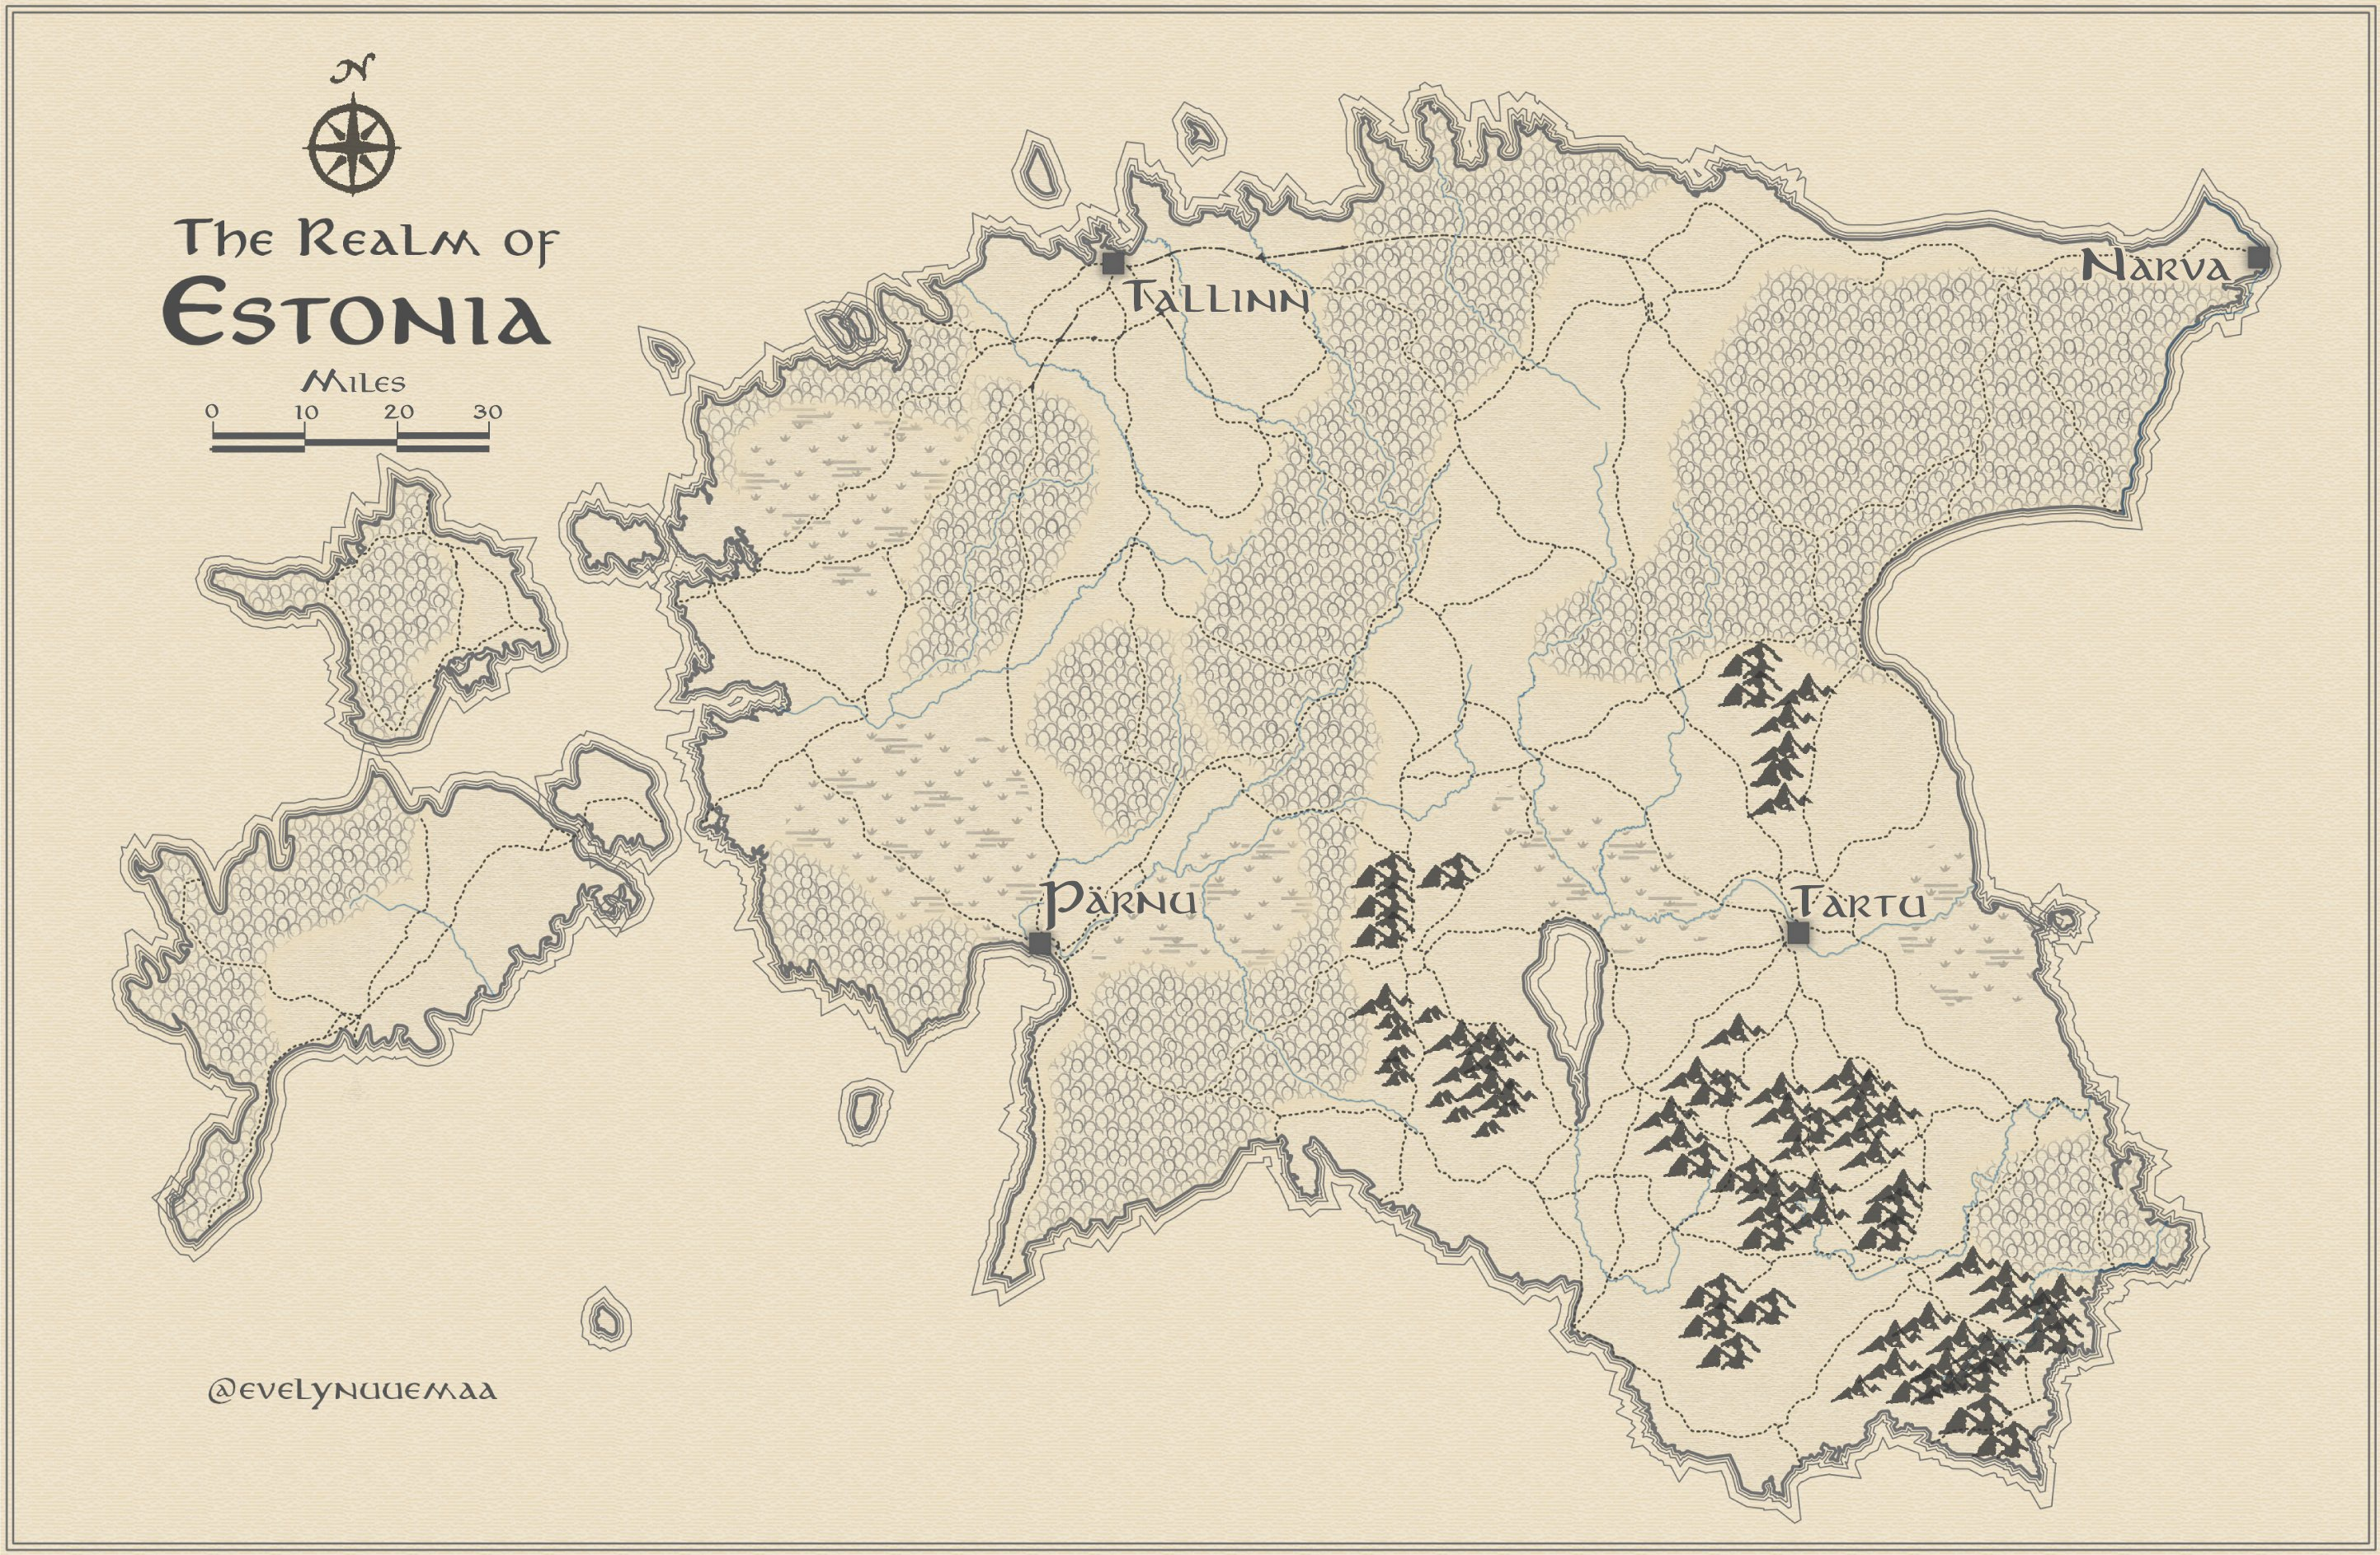
\includegraphics[width=1\linewidth]{C:/Users/a71386/Desktop/GeoHum/andres/geohumcourse/imgs/example_lotr_uuemaa}

\}

\textbackslash caption\{Eesti kujutatud Sõrmuste Isanda kaartide stiilis, \href{https://twitter.com/evelynuuemaa/status/1291261715095662592?s=07\&fbclid=IwAR1q6bpp4c7UNOTYph2YngZ7DrlBzrftR1gX2upWtoVNxLNzdFsgXZv_sVQ}{twitter.com/evelynuuemaa}\}\label{fig:lotr-map}
\textbackslash end\{figure\}

Geoinfosüsteem on \textbf{arvutipõhine süsteem ruumiliste ja mitteruumiliste andmete kogumiseks, haldamiseks, analüüsiks, visualiseerimiseks ja jagamiseks}. Selle abil on võimalik ruumisuhete kaudu mõista oma andmeid paremini või teisest vaatepunktist ning sedakaudu teha kaalutletumaid otsuseid.

\begin{figure}

{\centering 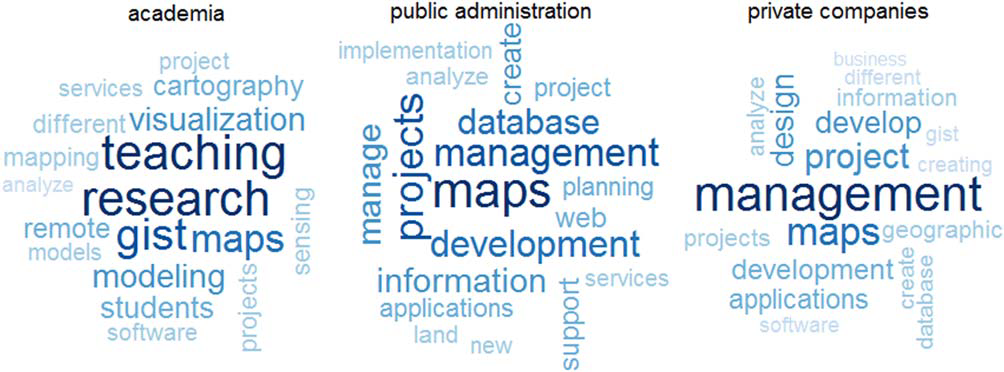
\includegraphics[width=0.8\linewidth]{C:/Users/a71386/Desktop/GeoHum/andres/geohumcourse/imgs/gis_wordcloud_wallentin2015} 

}

\caption{Mida GISiga tehakse? [@Wallentin2015, jn 4]}\label{fig:gis-wordcloud}
\end{figure}

\textbackslash begin\{figure\}

\{\centering 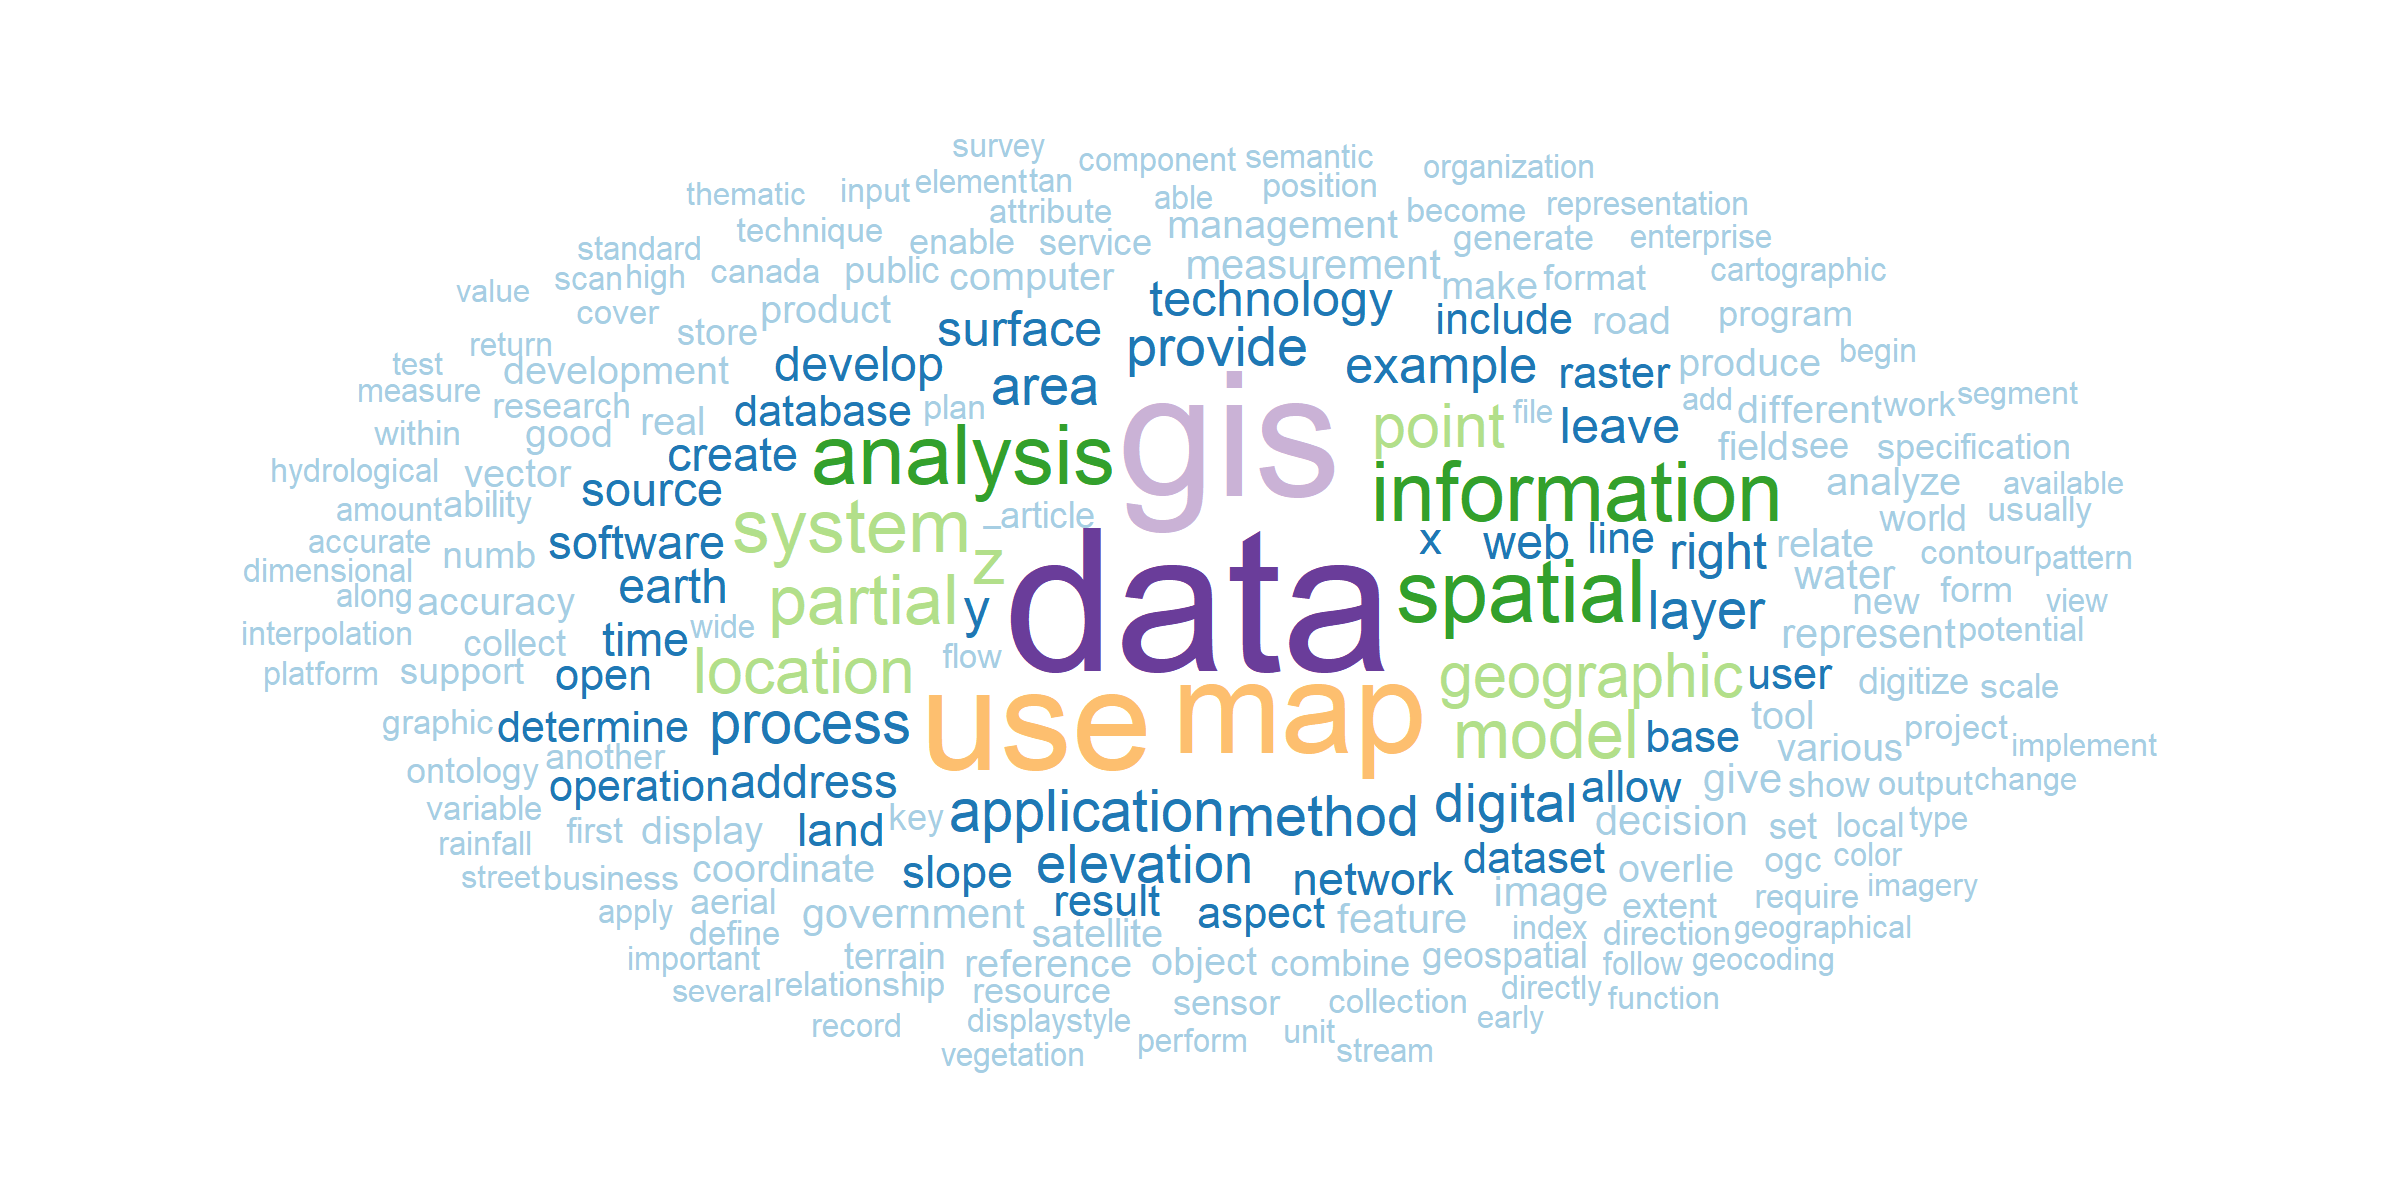
\includegraphics[width=0.8\linewidth]{C:/Users/a71386/Desktop/GeoHum/andres/geohumcourse/imgs/GISwordcloud}

\}

\textbackslash caption\{Sõnapilv Wikipedia artiklist `\href{https://en.wikipedia.org/wiki/Geographic_information_system}{Geographic information system}'\}\label{fig:gis-wordcloud2}
\textbackslash end\{figure\}

Andmete

\begin{itemize}
\tightlist
\item
  kogumine (nt paberkaartide digiteerimine, päringud repositooriumidest, käsitsi sisestamine);\\
\item
  haldamine (nt andmebaaside struktureerimine, dokumenteerimine);\\
\item
  analüüs (nt erinevate andmekihtide ühendamine, kattuvate alade arvutamine, puuduvate väärtuste arvutamine, puhveralade arvutamine);
\item
  visualiseerimine (nt kaartide koostamine ja kujundamine);
\item
  jagamine (nt projektide majutamine veebis, andmete ja metaandmete publitseerimine).
\end{itemize}

\textbackslash begin\{figure\}

\{\centering 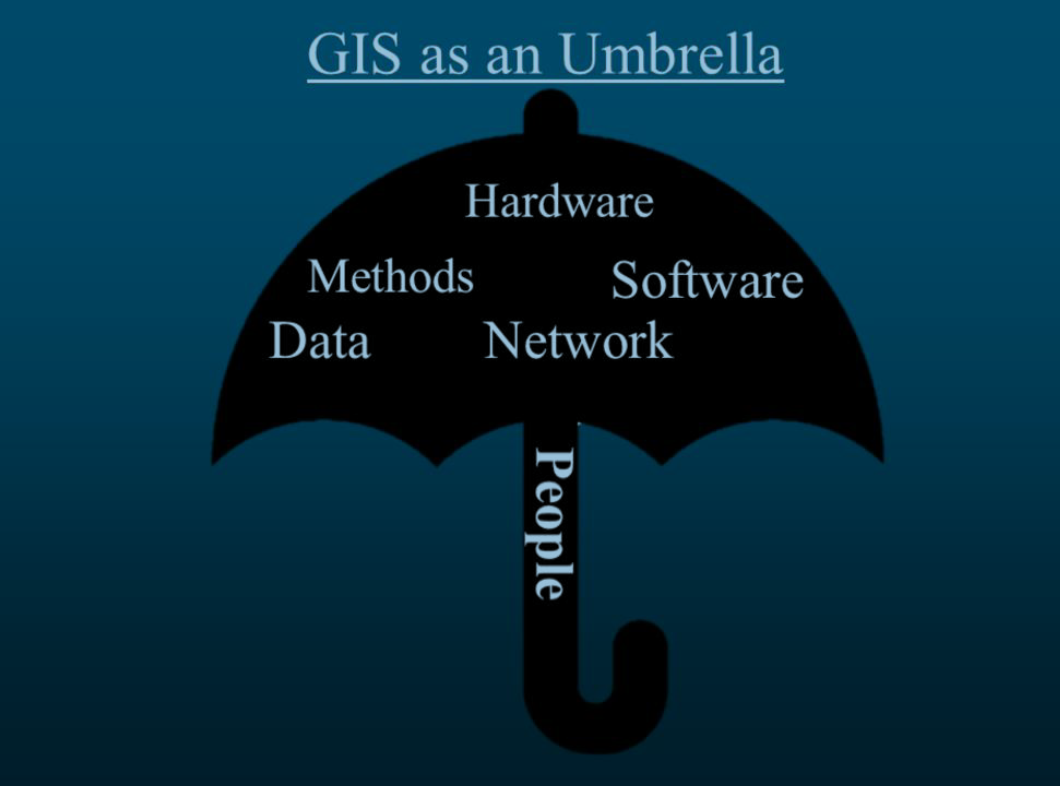
\includegraphics[width=0.75\linewidth]{C:/Users/a71386/Desktop/GeoHum/andres/geohumcourse/imgs/intro_GISumbrella}

\}

\textbackslash caption\{GIS kui vihmavari, \href{http://spatialquerylab.com/FOSS4GAcademy/Lectures/GST101/L1/1-What_are_Geographic_Information_Systems.pdf}{What are Geographic Information Systems}\}\label{fig:gis-umbrella}
\textbackslash end\{figure\}

Ehkki vahel käsitletakse geoinfosüsteeme kui mingit kindlat tarkvara (nt ArcView, MapInfo, ArcGIS), on GIS definitsioonilt pigem mingite funktsionaalsuste kogum. See tähendab ka seda, et erinevad tarkvarad või selle osad võivad spetsialiseeruda erinevatele funktsioonidele ning mingeid funktsioone (nt andmete kogumine) ei pea üldse tarkvara abil täitma.

\begin{figure}

{\centering 
\includegraphics[width=0.25\linewidth,height=0.5\textheight]{C:/Users/a71386/Desktop/GeoHum/andres/geohumcourse/imgs/arcgis_logo} 
\includegraphics[width=0.25\linewidth,height=0.5\textheight]{C:/Users/a71386/Desktop/GeoHum/andres/geohumcourse/imgs/qgis_logo} 
\includegraphics[width=0.25\linewidth,height=0.5\textheight]{C:/Users/a71386/Desktop/GeoHum/andres/geohumcourse/imgs/grassgis_logo} 
\includegraphics[width=0.25\linewidth,height=0.5\textheight]{C:/Users/a71386/Desktop/GeoHum/andres/geohumcourse/imgs/Rlogo} 

}

\caption{Populaarsed GIS tarkvarad}\label{fig:gis-tarkvarad}
\end{figure}

Kuigi GIS võib talletada ka mitteruumilist infot, moodustavad kõige olemuslikuma osa geoinfosüsteemidest siiski just ruumiandmed. Kõige sagedamini kasutatakse GISi geograafiliste andmete töötlemiseks, ent neid saab põhimõtteliselt kasutada mis tahes andmete jaoks, millel on mingid dimensioonid (nt väljamõeldud kohad; inimkeha; planeetide pinnad; puuviljad jne). Geoinfosüsteemidest võib seega kõige lihtsamal moel mõelda kui koordinaatidega varustatud andmebaasidest ja nende sisu analüüsimiseks ja visualiseerimiseks mõeldud tööriistadest.

\begin{figure}

{\centering 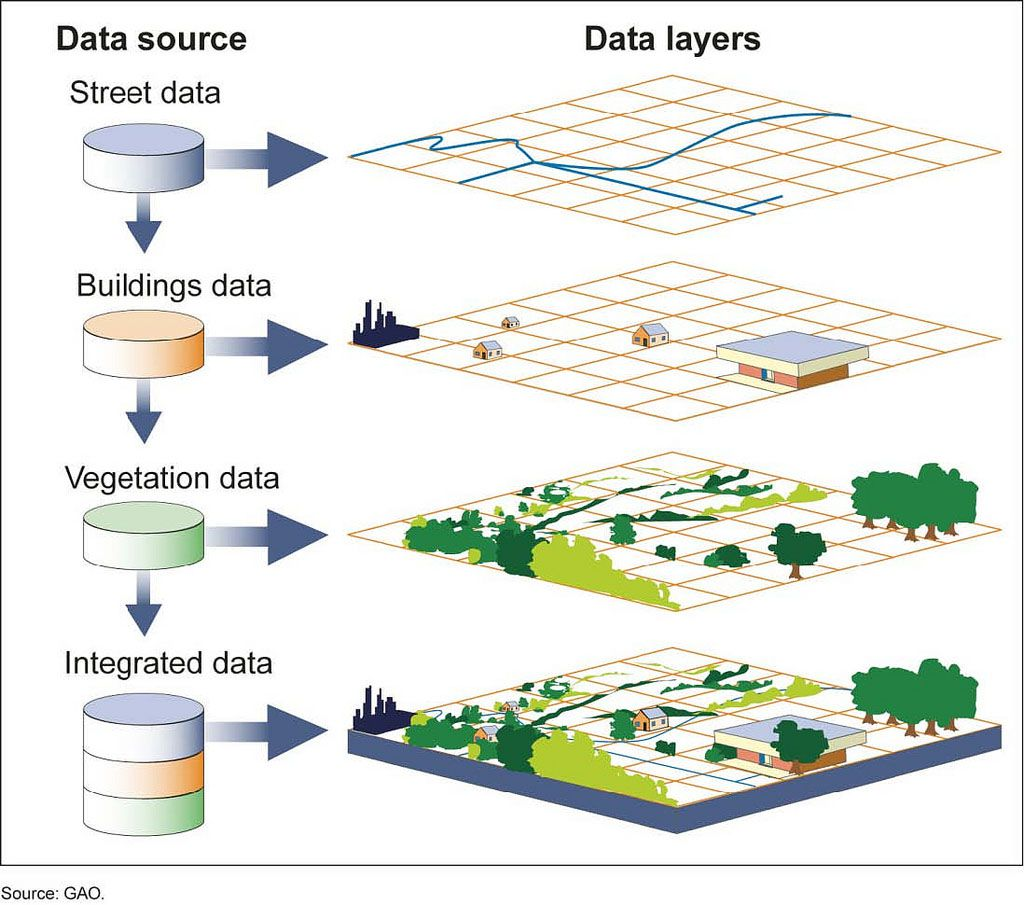
\includegraphics[width=0.75\linewidth]{C:/Users/a71386/Desktop/GeoHum/andres/geohumcourse/imgs/gis_natgeo} 

}

\caption{Andmete hoidmine GISis kihtidena, [GIS NatGeo](https://www.nationalgeographic.org/encyclopedia/geographic-information-system-gis/)}\label{fig:kihid}
\end{figure}

Nagu öeldud, võivad GIS-andmebaasid sisaldada nii ruumilist kui ka mitteruumilist infot. Ruumilist infot väljendatakse koordinaatidega (nt \emph{x}, \emph{y}, \emph{z}, pikkus- ja laiuskraad, kõrgus merepinnast) ning need määravad iga objekti asukoha, kasutades kas punkti, joont, polügooni või pikslit. Mitteruumilist infot, mis mingit kohaga seotud on, väljendavad \textbf{atribuudid}. Atribuudid on tüüpiliselt salvestatud tabelina, kus iga objekt on eraldi real ning iga atribuut eraldi tulbas, või mingis muus (nt hierarhilises) andmebaasistruktuuris.

\begin{figure}

{\centering 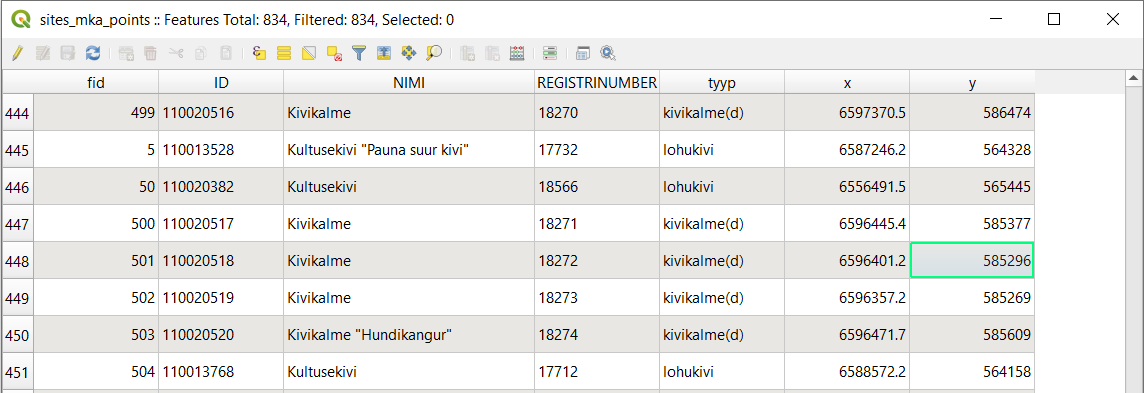
\includegraphics[width=1\linewidth]{C:/Users/a71386/Desktop/GeoHum/andres/geohumcourse/imgs/qgis_attribute_table} 

}

\caption{Näide QGISi atribuuttabelist}\label{fig:attribute-table}
\end{figure}

Infotehnoloogia arenguga on muutunud võimalikuks säilitada digitaalsel kujul atribuutidena peaaegu mis tahes tüüpi andmeid: nt struktureerimata tekste (raamatuid, veebilehti), pilte, videoid, helifaile. Kuna geoinfosüsteemid on arvutipõhised, nõuavad need siiski, et andmed oleksid mingil moel formaliseeritud. See tähendab ka vahel seda, et tuleb andmetele suruda peale jäigad kategooriad ka seal, kus kategooriatevahelised piirid on tegelikult sujuvad ning on palju üleminekualasid.

\hypertarget{geoinfosuxfcsteemide-ajaloost}{%
\section{Geoinfosüsteemide ajaloost}\label{geoinfosuxfcsteemide-ajaloost}}

\textbackslash begin\{figure\}

\{\centering 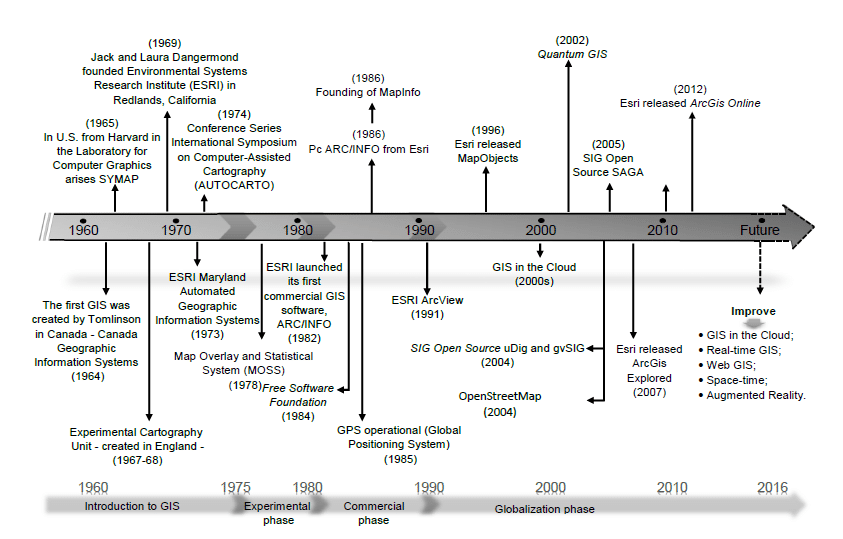
\includegraphics[width=1\linewidth]{C:/Users/a71386/Desktop/GeoHum/andres/geohumcourse/imgs/Timeline-of-major-GIS-events}

\}

\textbackslash caption\{\href{https://www.researchgate.net/figure/Timeline-of-major-GIS-events_fig1_315640751}{GISi ajajoon}\}\label{fig:ajajoon}
\textbackslash end\{figure\}

\begin{itemize}
\tightlist
\item
  Geoinfosüsteeme hakati arendama ja kasutama 1960ndatel, kui akadeemilistes ringkondades hakati uurima kvantitatiivse ja arvutusliku geograafia võimalusi.\\
\item
  GISi ``isaks'' peetakse Roger Tomlinsoni (1933-2014), kes 60ndate alguses arendas Kanadas välja kõige \textbf{esimese geoinfosüsteemi maailmas} (\emph{Canada Geographical Information System} CGIS). Süsteemi ülesandeks oli talletada, võrrelda ja analüüsida Kanada maakasutuse andmeid.
\end{itemize}

\begin{itemize}
\tightlist
\item
  GISi ulatuslikum areng toimus 1970ndatel ning 1980ndate lõpuks oli fookus juba sellel, kuidas parandada GISi kasutuskogemust.\\
\item
  Esimestel aastakümnetel oli GIS põhiliselt haldus- ja militaarkasutuses. 1981. aastal tõi Esri (Environmental Systems Research Institute, Inc.) välja \textbf{esimese kommertsliku GIS-toote}, ARC/INFO, mis põhines Harvard Laboratory Computer Graphicsi poolt arendatud esimesel vektoritega töötaval GISil. Esri roll GIS-tarkvara arendajana on sellest alates ainult kasvanud.\\
\item
  1990ndatest alates hakkas GISi \textbf{kasutajaskond kiiresti kasvama}. Seda soodustas järjest väiksemate, odavamate ja kiiremate arvutite tootmine, andmete ulatuslikum kättesaadavus ning uute satelliitide ja kaugseiretehnoloogia kasutuselevõtt.
\item
  Viimast kaht kümnendit on iseloomustanud lisaks tehnoloogia jätkuvale arengule ka \textbf{vabavaralise GIS-tarkvara teke}, mis on teinud ruumiandmete kasutamise ja analüüsi kättesaadavamaks nii tavakasutajale kui ka talle pakutavate toodete arendajatele. On toimunud nn \textbf{\href{https://www.e-education.psu.edu/maps/l1_p2.html}{georuumiline revolutsioon (\emph{Geospatial Revolution})}}, mis on muutnud nii seda, kuidas me liigume, otsuseid teeme ja oma lugusid jagame.
\end{itemize}

Praeguseks kasutatakse geoinfosüsteeme näiteks

\begin{itemize}
\tightlist
\item
  telekommunikatsioonis,
\item
  linnaplaneerimises (näiteks \href{https://lips.tallinn.ee/est}{Tallinna Ligipääsetavuse infosüsteem}),
\item
  logistikas, navigeerimises (näiteks \href{https://gis.vta.ee/nutimeri/}{Veeteede Ameti Nutimer}),
\item
  meteoroloogias,
\item
  katastroofide ohjamisel ja leevendamisel,
\item
  tervishoius,
\item
  kuritegevuse analüüsil,\\
\item
  \ldots{}
\end{itemize}

Vt veel rakendusvaldkondi nt \href{https://grindgis.com/blog/gis-applications-uses}{siit}.

\hypertarget{ruumiandmed-ja-gis-humanitaarteadustes}{%
\section{Ruumiandmed ja GIS humanitaarteadustes}\label{ruumiandmed-ja-gis-humanitaarteadustes}}

Ehkki näiteks arheoloogias on ruum ja ruumiandmed olnud alati kesksel kohal, on teistes humanitaaria valdkondades (nt ajaloos, kirjandusteadustes) toimunud viimase paarikümne aasta jooksul nn \textbf{ruumiline pööre} (\emph{Spatial Turn}). Ruumiline pööre algas tegelikult geograafia valdkonna seest: pelga inimelu või -tegevuse mahuti või ``lava'' tõlgenduse asemel seati fookusesse ruum kui pidevalt muutuv ja kompleksne sotsiaalne moodustis. See võimaldas leida enam ühist keelt ka sotsiaal- ja humanitaarteadlastega. Humanitaarteadustes on küll \emph{ruumi} ja \emph{koha} mõistetel olnud alati üsna prominentne roll, ent ruumilise pöörde käigus seati fookus eksplitsiitselt sellele, kuidas sotsiaalsete muutuste ning laiemalt inimtegevuse seletamiseks tuleb võtta arvesse ka ruumilist komponenti. Sealjuures rõhutatakse, et ruum võib ajas muutuda ning et \emph{ruumid} võivad olla nii füüsilis-geograafilised kui ka abstraktsed, metafoorsed või väljamõeldud (vt nt hiljutist Keele \& Kirjanduse erinumbrit \href{https://keeljakirjandus.ee/ee/issue/2020-8-9/}{``Keel ja ruum''}). Nõnda on näiteks keskaegses kirjanduses narratiivi loomise seisukohast võrdselt olulised nii London kui ka Camelot; erinevate keelte kaassõnu (nt \emph{ees}, \emph{kõrval}, \emph{taga}) uurides saame teada, kuidas mingi keele kõneleja end mõtteliselt millegi suhtes positsioneerib (kas absoluutselt või relatiivselt), kuidas tajutakse aega ruumisuhete kaudu jne).

Ruumi asetamine kesksele positsioonile on digihumanitaaria katusmõiste alla sünnitanud interdistsiplinaarsed valdkonnad nimega \textbf{geohumanitaaria} (\emph{GeoHumanities}) ja \textbf{ruumihumanitaaria} (\emph{Spatial Humanities}), mis ühendavad GISi ja klassikalised ruumianalüüsi meetodid (nt teekondade arvutamine, kaartide koostamine) uuemate arvutuslike meetoditega (nt loomuliku keele töötlus, võrgustikuanalüüs, simulatsioonimudelid, tehisnärvivõrgud). Ruumihumanitaaria ja geohumanitaaria vaheline piir ei ole päris selge ning sageli kasutatakse mõisteid sünonüümidena, samuti on mõlemal valdkonnal suur ühisosa inimgeograafiaga. Kui aga eristust tehakse, siis loetakse geohumanitaaria valdkonda pigem konkreetsete, geograafiliste kohtade ja ruumidega tegelevad uurimused ning ruumihumanitaaria alla ka uurimused, mis analüüsivad sümboolseid, ähmaseid või väljamõeldud ruume.

Ehkki mingites humanitaaria valdkondades (nt arheoloogia) on ka geoinfosüsteemid olnud kasutusel juba aastakümneid, on nende võimalusi hakatud teistes humanitaarteaduste harudes rohkem kasutama alles viimase kümne-viieteistkümne aasta jooksul. See on ühelt poolt seotud arvutite võimsuse ning tarkvara ja andmete kättesaadavuse plahvatusliku kasvuga, ent ka teatava suhtumise muutusega humanitaaride seas. Ehkki humanitaaria uurimisobjektid ja andmed on sageli ebatäpsed, hägusad, täpselt määramatud ja fragmentaarsed ning nende analüüs GISi abil pakub endiselt rohkelt väljakutseid, ei nähta tehnoloogias kõigest positivistlikku ja humanitaaraladele olemuslikult sobimatut analüüsivahendit. GISi väärtus humanitaarteadustele seisneb eeskätt selles, et kohainfo (nt kohanime või koordinaatide) kaudu on võimalik ühendada eri formaatides väga erinevat infot, seda visualiseerida ning erinevatest infokihtidest sünteesida uut teadmist. Sealjuures on nõuded absoluutsele täpsusele humanitaarias oluliselt leebemad.

\begin{figure}

{\centering 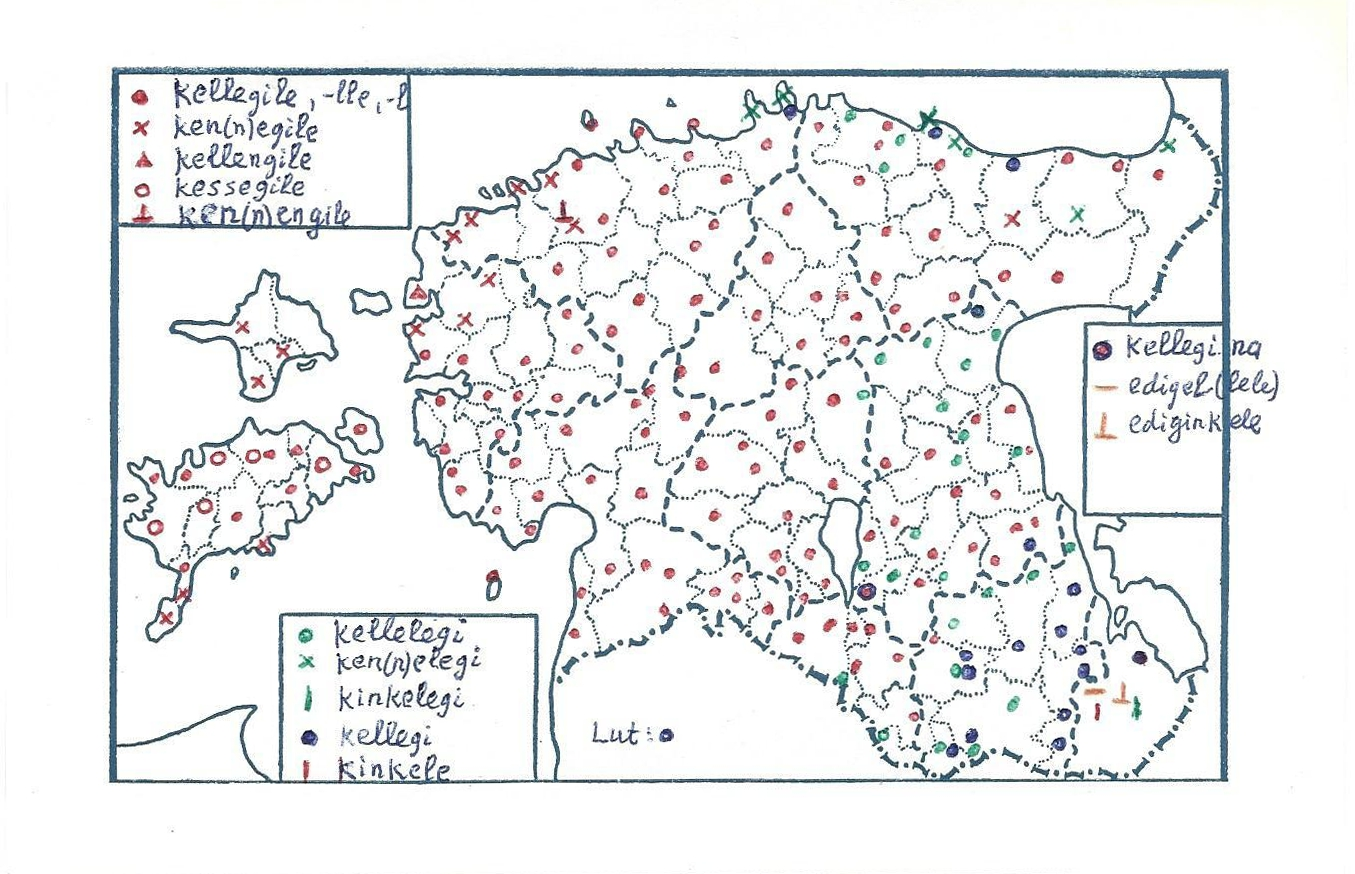
\includegraphics[width=1\linewidth]{C:/Users/a71386/Desktop/GeoHum/andres/geohumcourse/imgs/keegi_allatiiv} 

}

\caption{Andrus Saareste käsikirjaline murdekaart sõna 'keegi' alaleütleva käände ('kellelegi', 'kellegile' jm) varieerumisest. Vt rohkem kaarte [siit](http://rurake.keeleressursid.ee/index.php/andrus-saarestes-unpublished-dialect-maps/)}\label{fig:murdekaart}
\end{figure}

Geo- ja ruumihumanitaaria fookus ei ole aga pelgalt tehniliste analüüsimeetodite ja tööriistade kasutamisel ja arendamisel, vaid ka (või isegi eelkõige) ruumide ja kohtade teoreetilistel konstruktsioonidel ning nende muutumisel ajas ning eri kultuurides: kuidas mingites ruumides elatakse, kuidas mingeid ruume sotsiaalselt konstrueeritakse ja kuidas need ruumid omakorda mõjutavad majandust, poliitikat, kultuuri jne.

Siiski on vahest enamgi neid, kes ühel või teisel moel ruumiandmeid ja geoinfosüsteeme oma töös ära kasutavad, ilma et ennast või oma uurimistööd spetsiifiliselt ruumi- või geohumanitaaria valdkonna kaudu defineeriksid. Sellise üldise ruumiandmete analüüsi tööriistakasti koostamisega tegeleme ka siin kursusel.

\hypertarget{arheoloogia}{%
\subsection{Arheoloogia}\label{arheoloogia}}

\begin{figure}
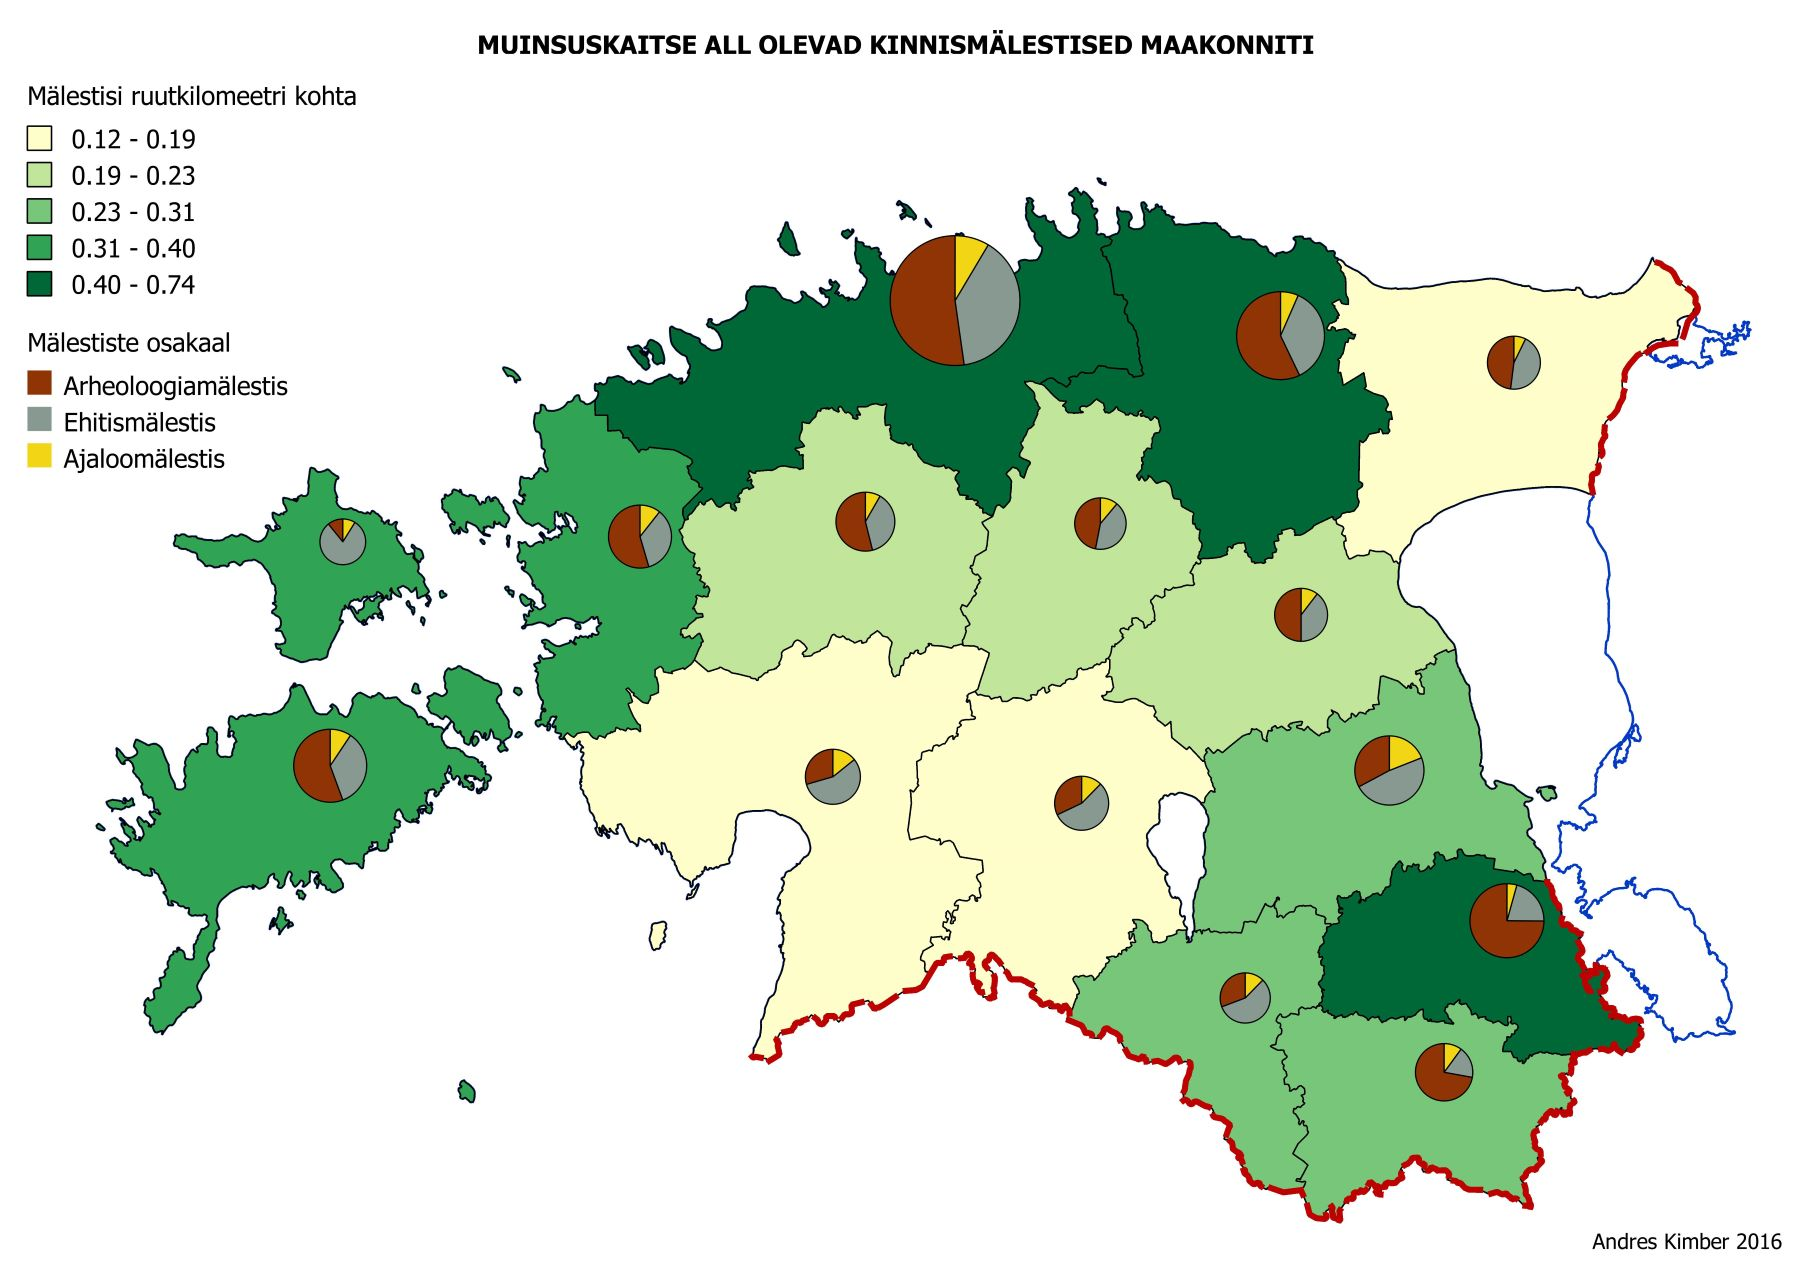
\includegraphics[width=1\linewidth]{C:/Users/a71386/Desktop/GeoHum/andres/geohumcourse/imgs/arheo_example_teemakaart_kimber} 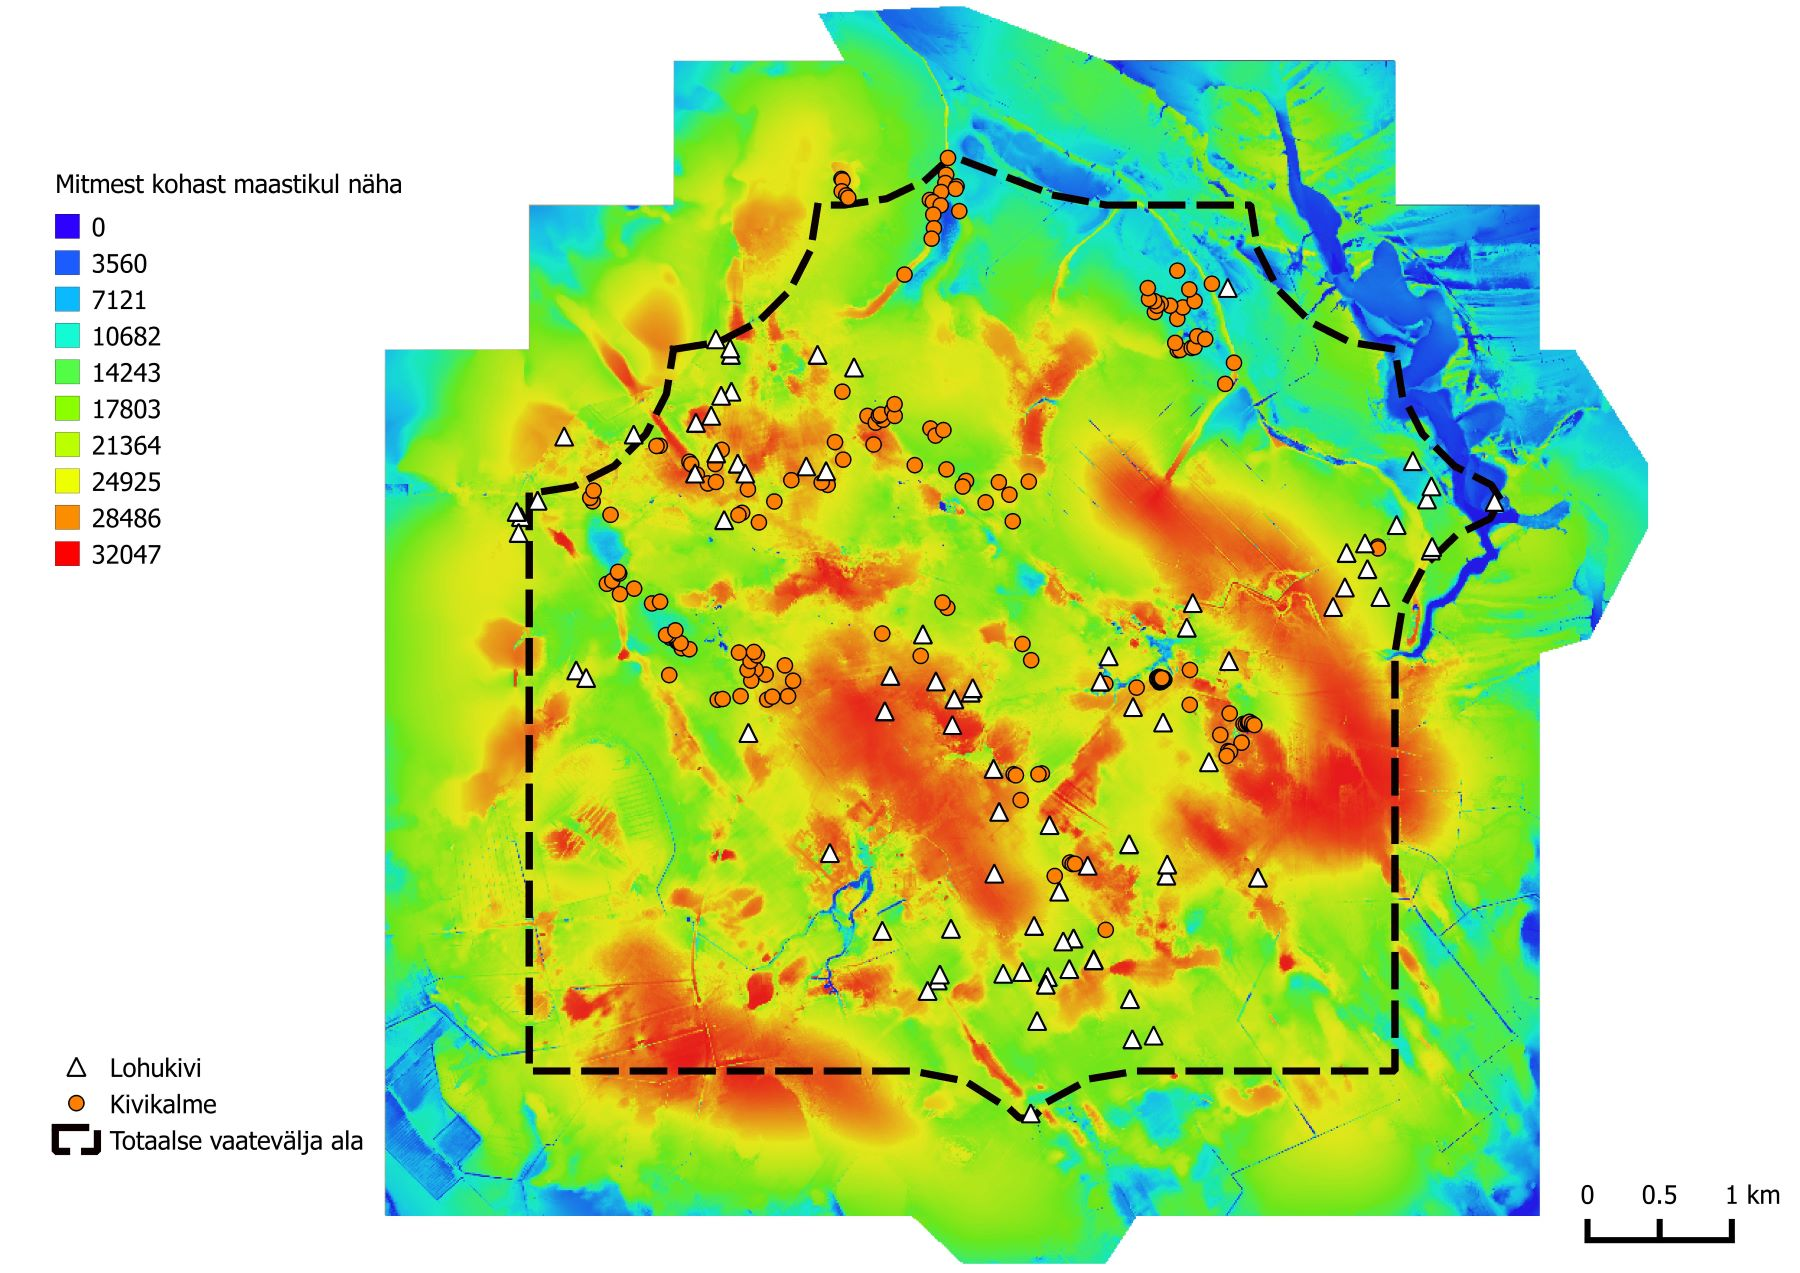
\includegraphics[width=1\linewidth]{C:/Users/a71386/Desktop/GeoHum/andres/geohumcourse/imgs/arheo_example_kimber_lohukivid_totalviewshed} \caption{Muististe jaotumise visualiseerimine  ja maastiku nähtavuse analüüsimine [@Kimber2016, jn 5]}\label{fig:arheo-example}
\end{figure}

\begin{figure}
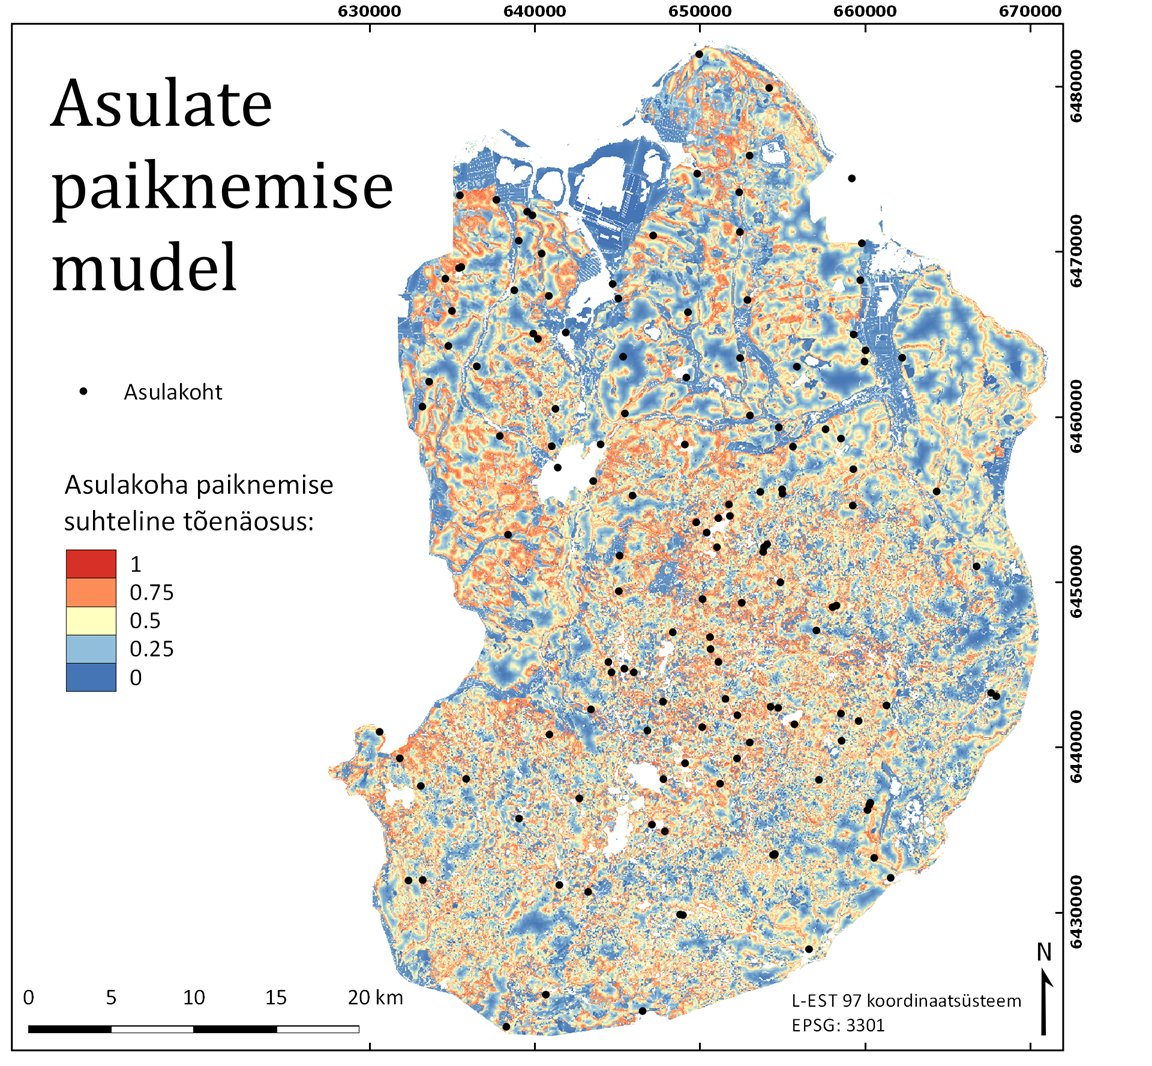
\includegraphics[width=1\linewidth]{C:/Users/a71386/Desktop/GeoHum/andres/geohumcourse/imgs/arheo_example_haav_asulate_mudel} 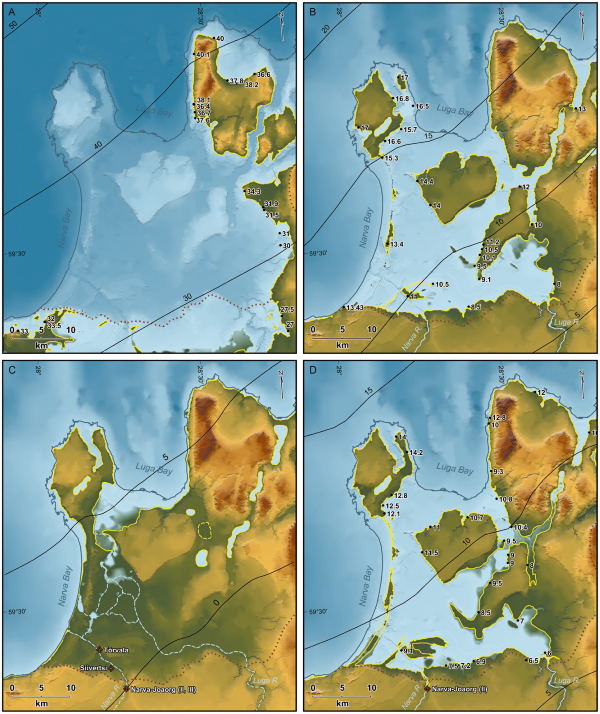
\includegraphics[width=1\linewidth]{C:/Users/a71386/Desktop/GeoHum/andres/geohumcourse/imgs/arheo_example_rosentau2013} \caption{Muinasaegsete asulakohtade ennustav mudeldamine [@Haav2014, jn 11] ja kiviaegse maastiku rekonstruktsioonid (9700 - 5300 eKr) [@Rosentau2013, jn 7]}\label{fig:arheo-example2}
\end{figure}

\hypertarget{veel-nuxe4iteid}{%
\subsection{Veel näiteid}\label{veel-nuxe4iteid}}

\begin{figure}

{\centering 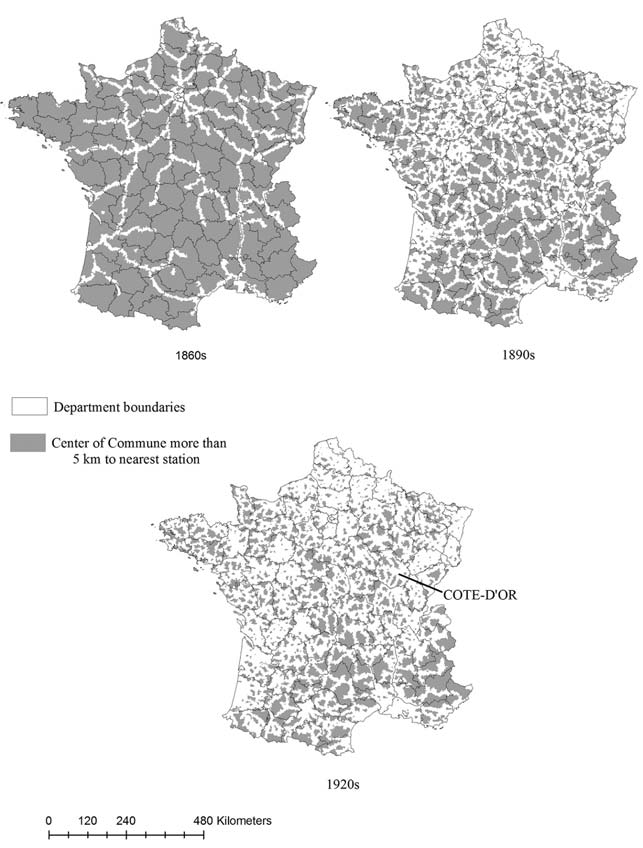
\includegraphics[width=0.75\linewidth]{C:/Users/a71386/Desktop/GeoHum/andres/geohumcourse/imgs/example_france_trains_geddes2014} 

}

\caption{Rongiliikluse areng Prantsusmaal [@Gregory2014, jn 1.3]}\label{fig:more-examples1}
\end{figure}

\begin{figure}

{\centering 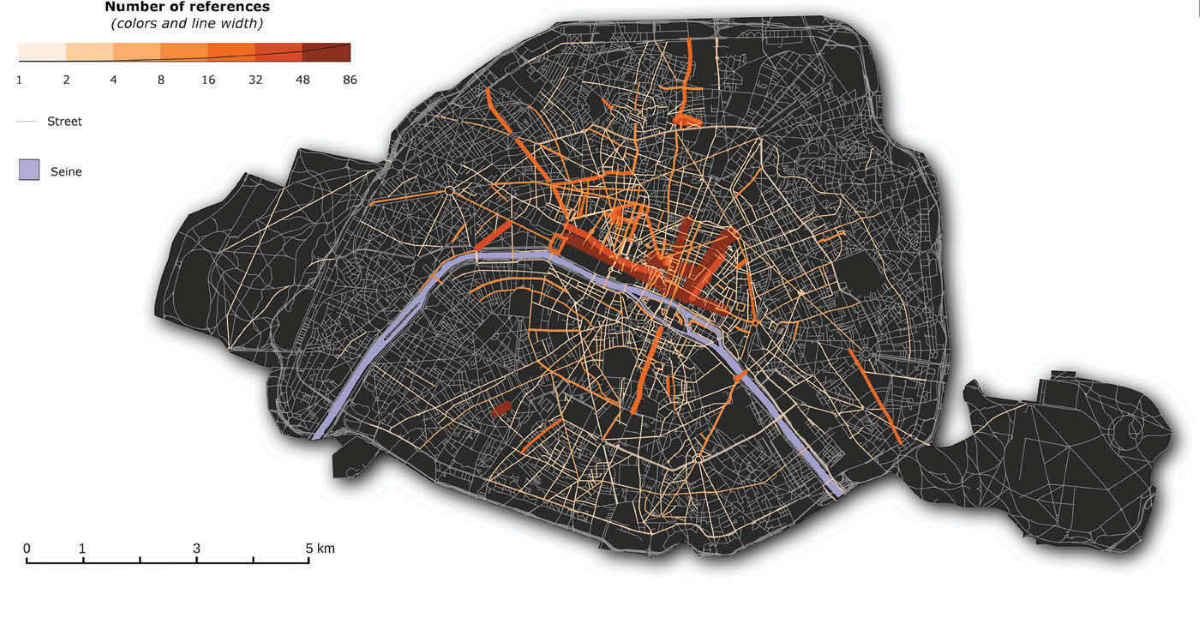
\includegraphics[width=1\linewidth]{C:/Users/a71386/Desktop/GeoHum/andres/geohumcourse/imgs/example_moncla_paris_street_mentions} 

}

\caption{Pariisi tänavate nimetamine kirjanduses [@Moncla2019, jn 4]}\label{fig:more-examples2}
\end{figure}

\hypertarget{kuxfcsitlus}{%
\section{Küsitlus}\label{kuxfcsitlus}}

Palun täida Moodle'is lühike küsimustik.

\hypertarget{juxe4rgmisel-korral}{%
\section{Järgmisel korral}\label{juxe4rgmisel-korral}}

Seminar.

Lugemiseks:

\begin{itemize}
\tightlist
\item
  Martyn Jessop \citeyearpar{Jessop2008}. \emph{The Inhibition of Geographical Information in Digital Humanities Scholarship}
\item
  Todd Presner \& David Shepard \citeyearpar{Presner2015}. \emph{Mapping the Geospatial Turn}
\end{itemize}

Artiklite pdf-id leiad Moodle'ist.

\emph{Arutlemiseks}

\begin{itemize}
\tightlist
\item
  Milliseid võimalusi geoinfosüsteemid humanitaariale pakuvad?\\
\item
  Milliseid humanitaarteaduste ja GISi põrkumise probleemkohti artiklites kirjeldatakse?\\
\item
  Kas need probleemkohad on maailma kontekstis endiselt aktuaalsed? Aga Eesti kontekstis?\\
\item
  Milliseid murekohti näed arvutuslike meetodite ja arvutipõhiste tehnoloogiate laiema leviku juures humanitaarteadustes?\\
\item
  Kas humanitaarteadused on omavahel ühildatavad? Aga teiste valdkondadega? Milline on interdistsiplinaarsete uurimuste/projektide olevik, milline tulevik?
\end{itemize}

\hypertarget{kirjandus}{%
\section{Kirjandus}\label{kirjandus}}

\hypertarget{seminar}{%
\chapter{Seminar}\label{seminar}}

\hypertarget{muxf5isted}{%
\section{Mõisted}\label{muxf5isted}}

Mõne artiklis kasutatud mõiste seletusi:

\begin{itemize}
\tightlist
\item
  \textbf{\emph{Cognitive maps}} - kujutluskaart. Inimese (või muu elusolendi) kogemuste põhjal ajju talletatud ettekujutus/mudel mingist reaalsest või irreaalsest ruumist; laiemas käsituses mis tahes protsessist või mõistest.\\
\item
  \textbf{\emph{Community mapping}}, \textbf{\emph{participatory mapping}} - kogukondlik ja/või osaluskaardistamine. Kaartide tegemine n-ö tavaliste inimeste poolt tavaliste inimeste jaoks, praktikas sageli mingil ühiskondlikul-kultuurilisel või poliitilisel eesmärgil (nt pärandi, keele kaitsmiseks, mingi kogukonna arengu planeerimiseks, mingi piirkonna ressursside õiglasemaks jaotamiseks). Nende mõistetega on lähedalt seotud ka mõiste \textbf{\emph{counter-mapping}}, mis veelgi selgemalt tegeleb alternatiivse kaardistamise abil traditsiooniliste võimusuhete lammutamise ja õõnestamisega. Nii osaluskaardistamine kui ka \emph{vastukaardistamine} esindavad \textbf{\emph{kriitilise kartograafia}} rakendusi. Kriitilise kartograafia põhitees on, et kaardid peegeldavad ja kinnistavad võimusuhteid ning seda enamasti ühiskonnas domineeriva klassi positsioonilt.\\
\item
  \textbf{\emph{Gazetteer}} - kohanimeloend. Koondab tavaliselt infot kohanimega seotud koordinaatide ja koha tüübi kohta (nt mägi, jõgi, linn, küla), aga võib lisaks sisaldada ka nt rööpnimekujusid, asustuse infot, seoseid teiste sõnastiku kirjetega jm infot.\\
\item
  \textbf{\emph{Geocoding}} - geokodeerimine ehk kohtade tekstiliste viidete (nt kohanimede, aadresside) muutmine geograafilisteks koordinaatideks. Tagurpidi geokodeerimine muudab omakorda geograafilised koordinaadid kohanimedeks või aadressideks.\\
\item
  \textbf{\emph{Locative media}} - 1) digitaalne sisu (nt pildid, videod, helid) või selle loomiseks kasutatud vahendid, millele on lisatud asukohainfo; 2) vahendid, mis kasutavad digitaalse sisu edastamiseks asukohainfot. Digihumanitaaria kontekstis ka raamistik, mille kaudu uurida üksikisiku suhteid ja vastastikuseid mõjusid koha ja tehnoloogiaga.\\
\item
  \textbf{\emph{Psychogeography}} - kunsti- ja teadussuund, mille fookuses on see, kuidas kogetakse (eeskätt) linnakeskkondi ning kuidas keskkond mõjutab meie emotsioone ja käitumist. Sealjuures pööratakse tähelepanu viisidele, kuidas saada ümbritsevast uusi ja ootamatuid elamusi ning avastada ``tavapärasest erinevat''.\\
\item
  \textbf{\emph{Thick mapping}} - paljude erinevate geograafiliste või kohaspetsiifiliste andmete (pildid, narratiivid, kaardid, suulised ja kirjalikud mälestused jne) kogumine, koondamine/agregeerimine ja visualiseerimine selleks, et pakkuda kohtadele ja neis toimunud sündmustele erinevaid perspektiive (ka nt millegi alusel marginaliseeritud või vähem häälekate gruppide omi). Kasutatud on ka terminit \emph{deep mapping}.
\end{itemize}

\hypertarget{ruxfchmatuxf6uxf6-1-gisi-ja-ruumi-geohumanitaaria-projekte-ja-rakendusi}{%
\section{Rühmatöö 1: GISi ja ruumi-/geohumanitaaria projekte ja rakendusi}\label{ruxfchmatuxf6uxf6-1-gisi-ja-ruumi-geohumanitaaria-projekte-ja-rakendusi}}

Võite osaleda üksi või rühmaga (maksimaalselt 3 inimest).

Otsige üks enda erialaga (lähemalt või kaugemalt) seotud projekt, mis kasutaks GISi või tegeleks ruumi- või geohumanitaariaga. Alustada võib näiteks \href{https://anterotesis.com/wordpress/mapping-resources/dh-gis-projects/}{siit}, aga kindlasti võiks lähemalt uurida ka artiklites olnud viiteid.

Lisage \href{https://padlet.com/maarjaliisapilvik/14fuhzi8dpw9i2to}{virtuaalsele tahvlile}:

\begin{itemize}
\tightlist
\item
  projekti nimi,
\item
  projekti link,
\item
  valdkond,\\
\item
  kirjeldus selle kohta, millega projektis tegeletakse,\\
\item
  võimalusel visuaalset lisamaterjali (nt pilte rakendustest, kaartidest vm).
\end{itemize}

\begin{figure}
\centering
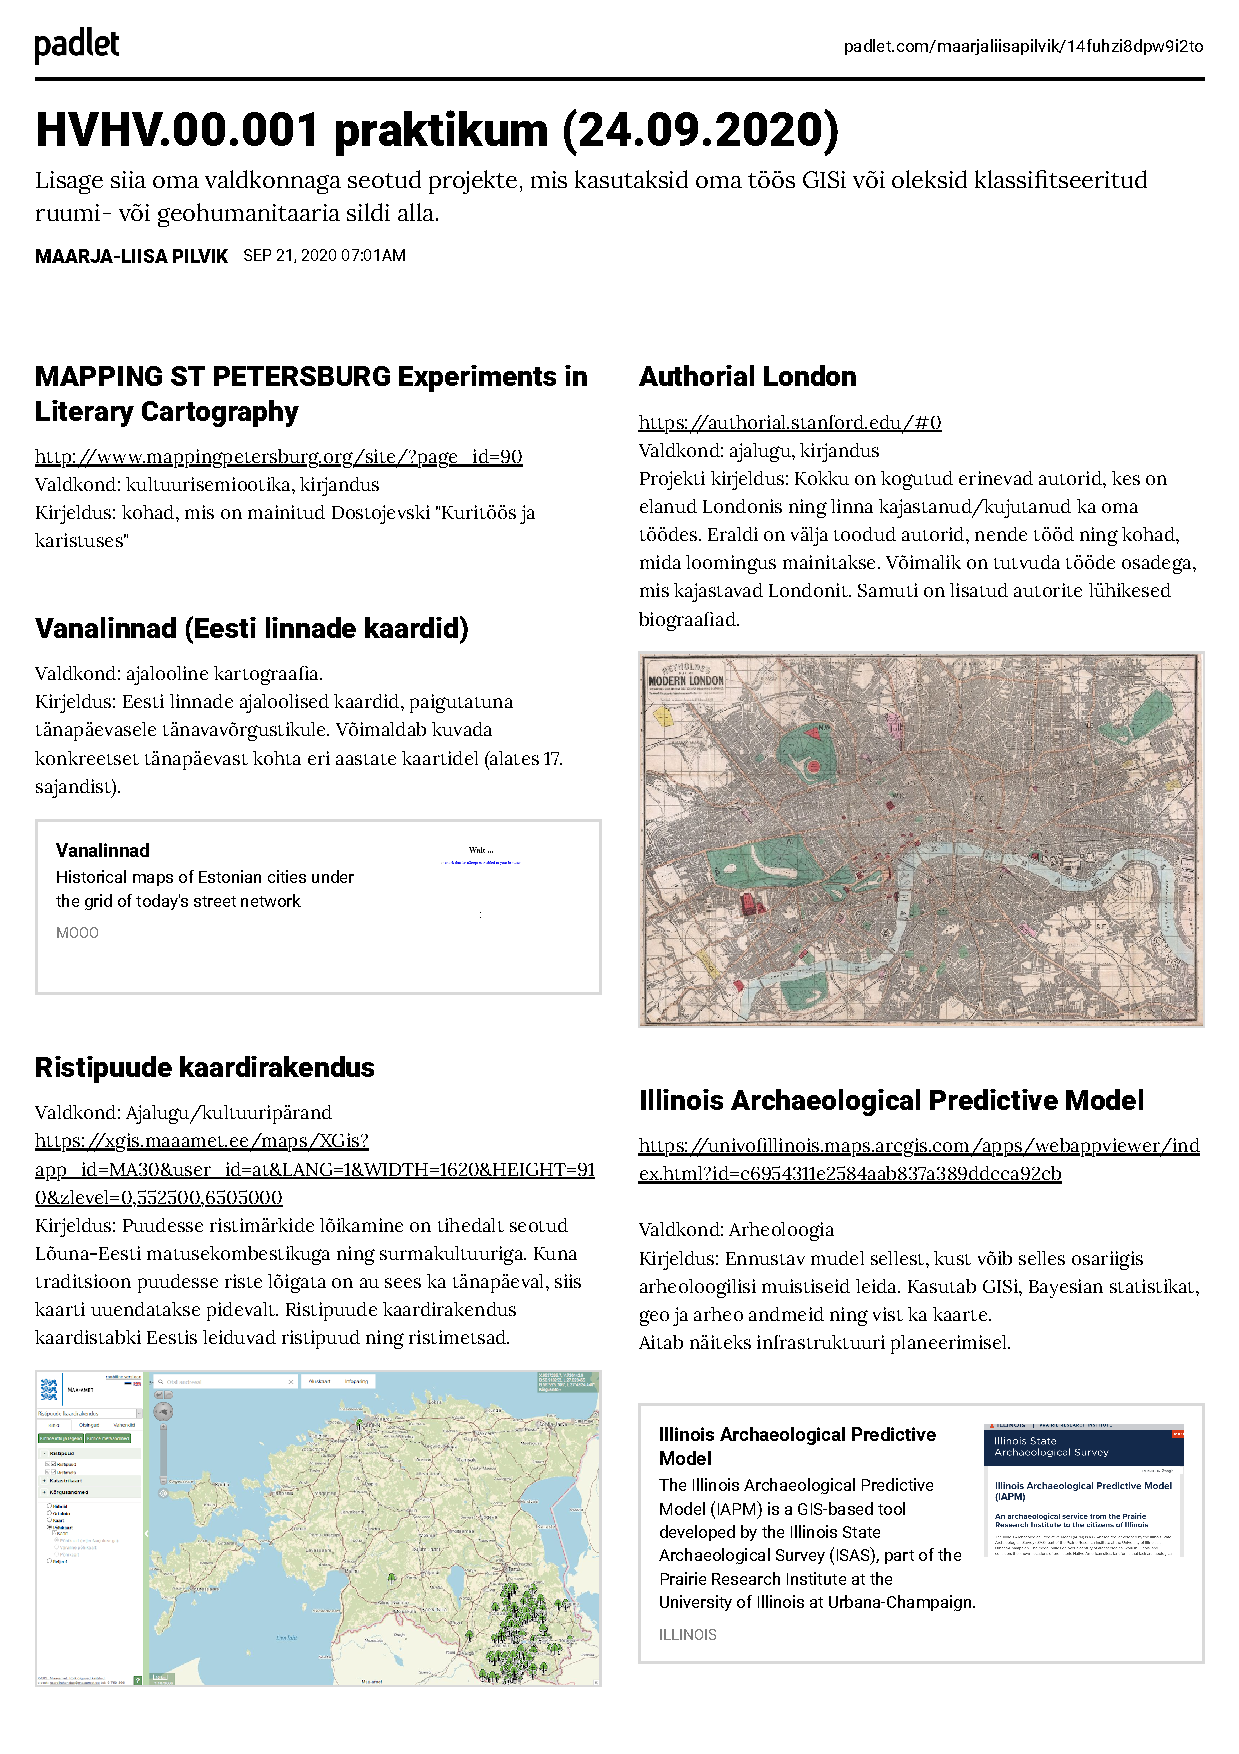
\includegraphics[width=1\textwidth,height=7.29167in]{./imgs/padlet_projektid.pdf}
\caption{Erinevaid projekte}
\end{figure}

\hypertarget{ruxfchmatuxf6uxf6-2-humanitaaria-vs.-kvantitatiivsed-meetodid}{%
\section{Rühmatöö 2: humanitaaria vs.~kvantitatiivsed meetodid}\label{ruxfchmatuxf6uxf6-2-humanitaaria-vs.-kvantitatiivsed-meetodid}}

Moodustage 3 inimesest koosnevad rühmad.

Pooled rühmad saavad \textbf{skeptikute/pessimistide} rolli: teie arvates ei saa GISi ja laiemalt praeguste arvutuslike meetodite ja kvantitatiivse lähenemisega humanitaaria andmete ja küsimustega töötada (või siis mitte vähemalt väga hästi). Ka interdistsiplinaarsus on teie meelest praktikas väga raskesti saavutatav.

Teine pool rühmadest saab \textbf{optimistide} rolli: teie arvates on humanitaaria eri suunad ka metodoloogiliselt pidevas arengus ning analüüsimeetodite vahetamine, laenamine ja kohandamine eri distsipliinide vahel ja sees annab humanitaariale väga palju juurde.

Koondage \href{https://padlet.com/maarjaliisapilvik/irf5y9aiahqkr9s1}{siia} võimalikult palju argumente ja lihtsalt arvamusi, näiteid jm, mis teie rühma esindatavat seisukohta toetaksid. Võite sealjuures loomulikult ära kasutada artikleid, guugeldada, aga ka rühma sees ise ideid genereerida.

\begin{figure}
\centering
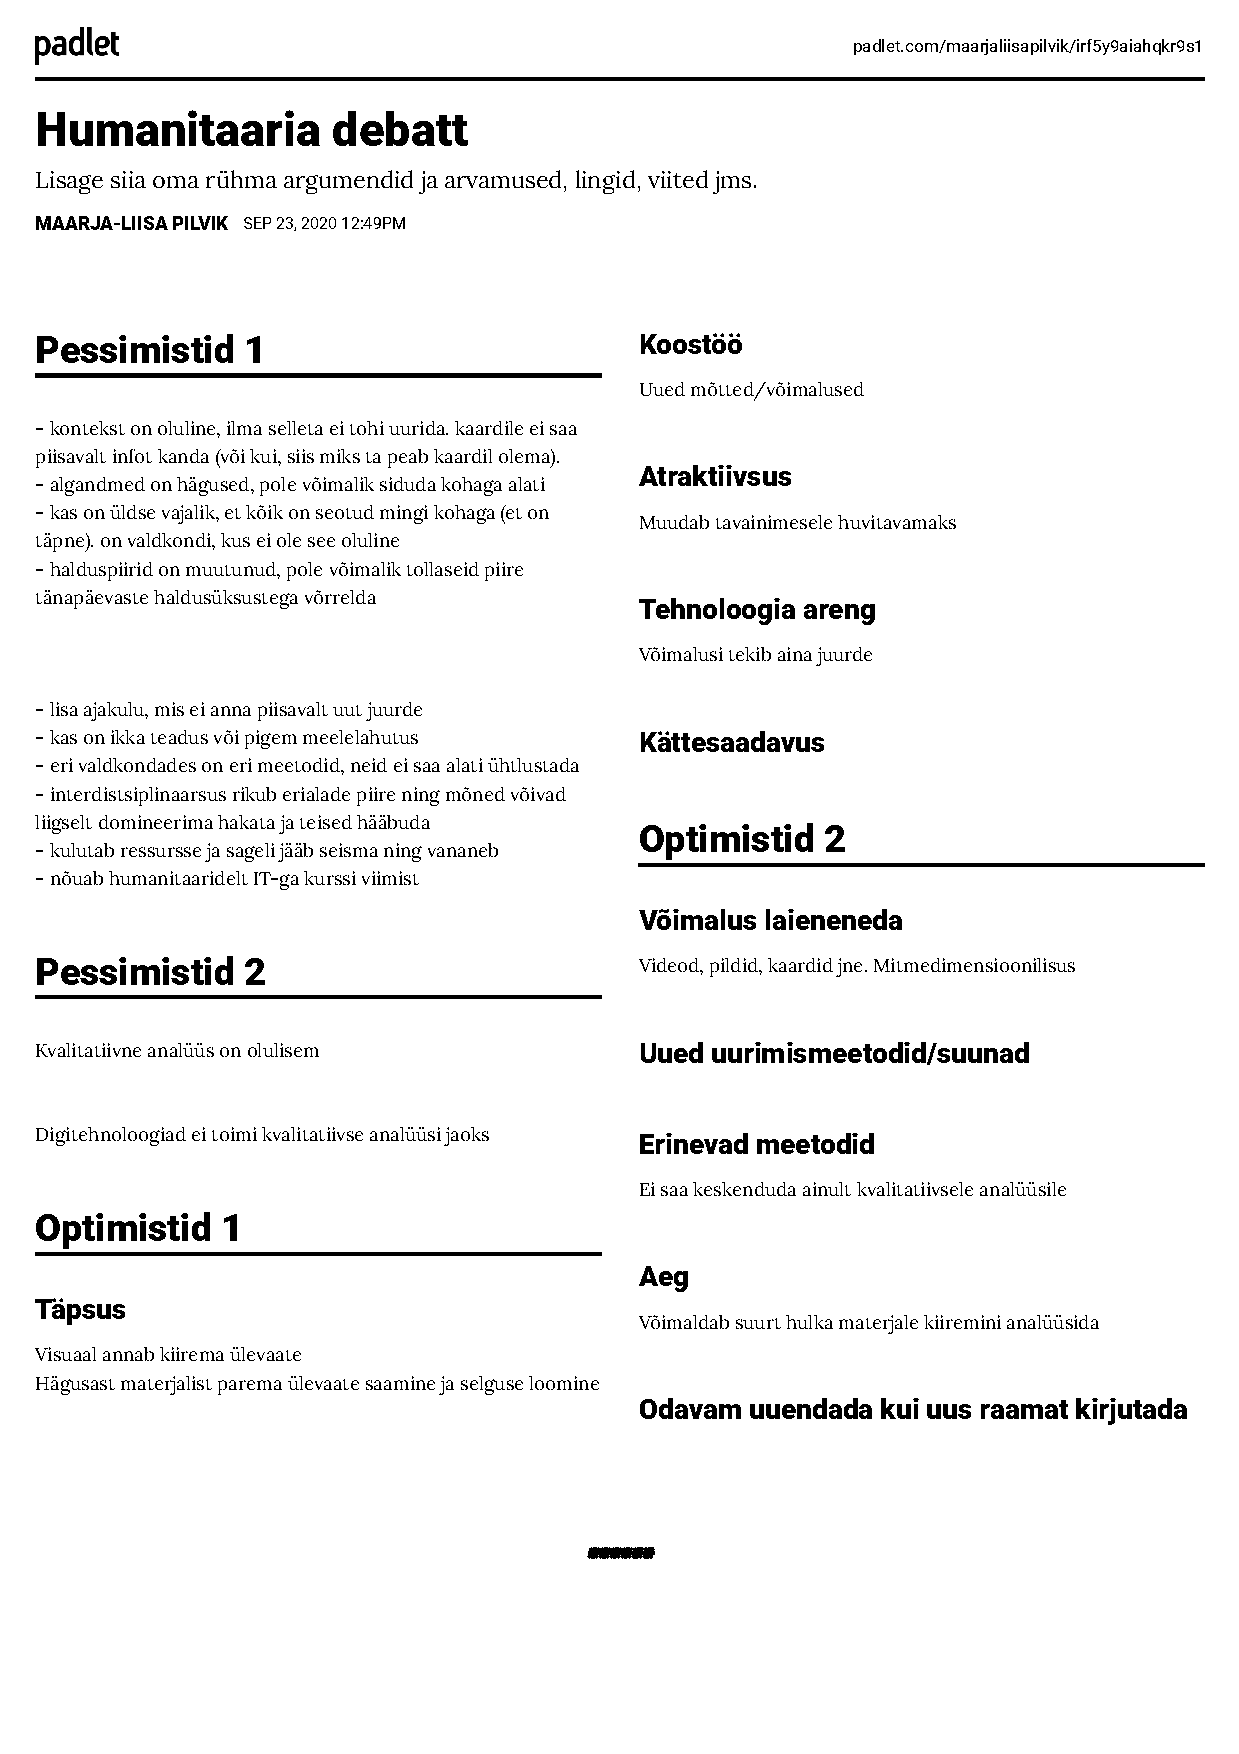
\includegraphics[width=1\textwidth,height=7.29167in]{./imgs/padlet-debatt.pdf}
\caption{Debatt}
\end{figure}

\hypertarget{ruumiobjektid}{%
\chapter{Ruumiobjektid ja ruumiandmed}\label{ruumiobjektid}}

Meid ümbritsevas maailmas on palju erinevaid ruumiga seotud nähtusi, näiteks konkreetsed füüsilised objektid (nt teed, hooned), kokuleppelised või abstraktsed objektid (nt riigipiir), sündmused (nt katastroofid, meeleavaldused, spordiüritused) või ka mingid pidevad nähtused, nagu temperatuur, mis esinevad väljana terves ruumis ning mille konkreetset väärtust on mingites ruumi punktides võimalik määrata.

Humanitaarteaduste kontekstis võime mõelda ka sellistest ruumiga seotud nähtustest ja objektidest, nagu muistsed ohverdusrituaalid, kirjandusteoste sündmused, (tajutavad) murdepiirid, ajaloolised lahingud, sõjakäigud jne.\\
Nähtustel on omakorda mingid omadused, mille abil neid nähtusi või ruumi ennast kirjeldada.

(Geo)infosüsteemide abil saame reaalse maailma objekte ja nähtusi hallata, kujutada ja analüüsida aga ainult nende mingil moel abstraheeritud ja formaliseeritud kujul, \textbf{ruumiobjektina}.

\href{https://www.riigiteataja.ee/akt/RAS}{Ruumiandmete seaduse} definitsioon (§ 3, lg 3):

\begin{quote}
Ruumiobjekt käesoleva seaduse tähenduses on konkreetse asukoha või geograafilise alaga seotud reaalmaailma nähtuse abstraktne kujutis.
\end{quote}

\textbf{Ruumiandmed} omakorda kirjeldavad

\begin{quote}
\ldots{} ruumiobjektide asukohta, omadusi ja kuju geograafilises ruumis.
\end{quote}

(Ruumiandmete seaduse § 3, lg 1.)

Objektidele ja nähtustele sobiva kujutamisviisi valimine sõltub eeskätt sellest, kas läheneme ruumile ja selles asuvatele objektidele ja nähtustele objektikeskselt või asukohakeskselt.

\begin{itemize}
\tightlist
\item
  \textbf{Objektikeskses} lähenemises seame fookusesse objektid. Need täidavad kindlates punktides mingit ruumi, neid saab loendada, need võivad külgneda ja kattuda, neil on mingid kindlad omadused, need on võib-olla seotud mingite teiste objektidega jne. Ruum ja selle omadused on ainult üks atribuut, mille kaudu objekte kirjeldada.

  \begin{itemize}
  \tightlist
  \item
    Sellises lähenemises on objektid \textbf{diskreetsed}: neil on kindel asukoht ja ruumikuju (nt hoone, mälestusmärk, riigipiir).\\
  \end{itemize}
\item
  \textbf{Asukohakeskses} lähenemises on fookus ruumil. Ruum on sama objektiga otsast otsani täidetud. Objektid ja nende omadused kirjeldavad ruumi, on ruumi atribuutideks.

  \begin{itemize}
  \tightlist
  \item
    Asukohakeskses lähenemises on objektid \textbf{pidevad}: objekt esineb terves ruumis, aga saab ruumi erinevates punktides erineva väärtuse (nt maapinna reljeef, temperatuur ja õhurõhk maapinnal, kultuurikihi intensiivsus).
  \end{itemize}
\end{itemize}

Need kaks lähenemist on aluseks sellele, kuidas ruumiobjekte geoinfosüsteemis kujutada: kas vektorkujul või rasterkujul. Vastavaid kujutusviise nimetatakse ka \textbf{ruumiandmete mudeliteks}.

\begin{figure}

{\centering 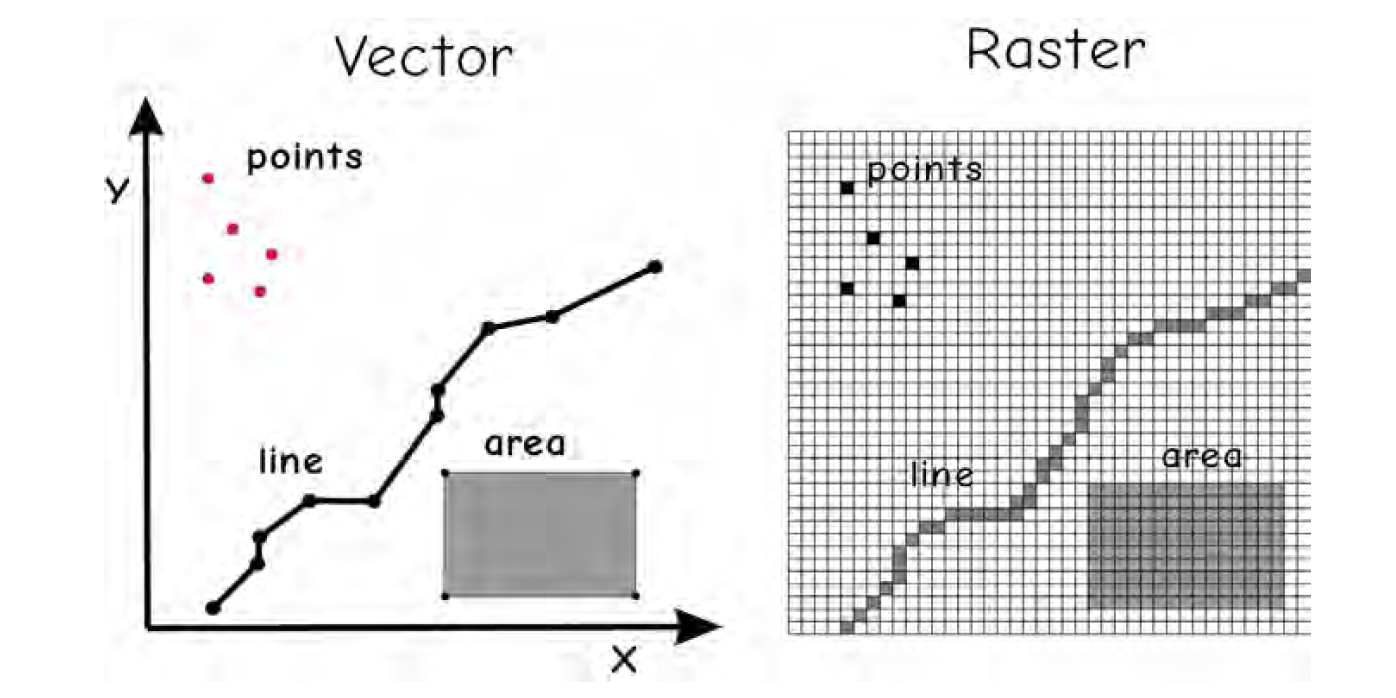
\includegraphics[width=1\linewidth]{C:/Users/a71386/Desktop/GeoHum/andres/geohumcourse/imgs/Bolstad2016} 

}

\caption{Vektor- vs. rasterandmed [@Bolstad2016 : 41]}\label{fig:data-models}
\end{figure}

\hypertarget{vektorandmed}{%
\section{Vektorandmed}\label{vektorandmed}}

\textbf{Vektormudelis} kujutatakse andmeobjekte (st reaalse või miks mitte ka kognitiivse maailma objekte ja nähtusi) \textbf{geomeetriliste kujundite} abil.
Geomeetrilisi põhiobjekte ehk primitiive on 3:

\begin{itemize}
\tightlist
\item
  \textbf{punkt} (nt torn, kivi)\\
\item
  \textbf{joon} (nt tee, jõgi)\\
\item
  \textbf{pind/areaal/polügoon/ala/kontuur} (nt põld, mets, linn)
\end{itemize}

\begin{figure}

{\centering 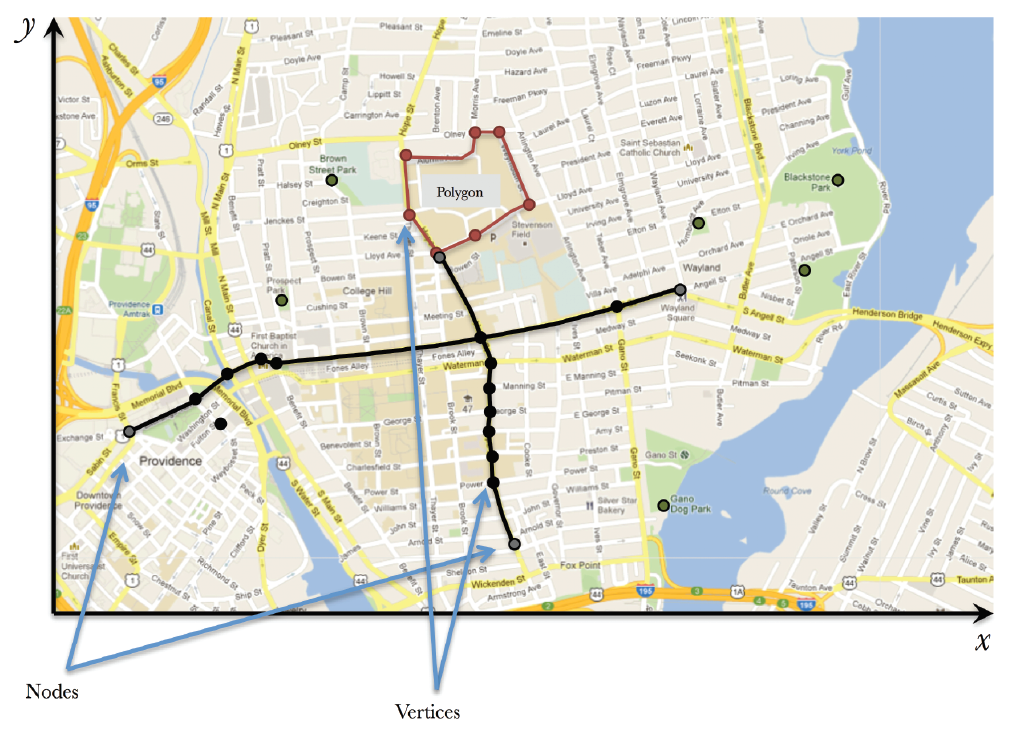
\includegraphics[width=1\linewidth]{C:/Users/a71386/Desktop/GeoHum/andres/geohumcourse/imgs/points_lines_polygons} 

}

\caption{Punktid, jooned, polügoonid [@Ballas2018 : 13]}\label{fig:ruumiobjektid}
\end{figure}

\textbf{Punkt} on eukleidilises mõttes nullmõõtmeline ning seda esitatakse koordinaatsüsteemis kujul \emph{P}(x; y).

Mitmest punktist moodustub ühemõõtmeline \textbf{joon}, enamasti \emph{murdjoon}, mille (käänu)punktid saab ühendada sirglõiguga.

Joon(t)est omakorda saab moodustada \textbf{polügooni}, mispuhul joone algus- ja lõpp-punkt kattuvad.

\begin{figure}

{\centering 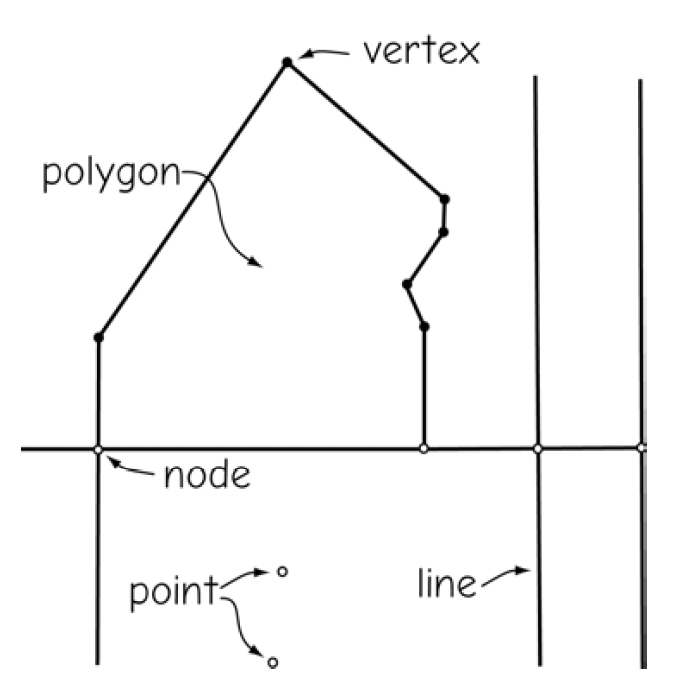
\includegraphics[width=0.6\linewidth]{C:/Users/a71386/Desktop/GeoHum/andres/geohumcourse/imgs/Bolstad2016_pointslinespolygons} 

}

\caption{Geomeetrilised objektid [@Bolstad2016 : 43]}\label{fig:points-lines-polygons}
\end{figure}

Geomeetrilise objekti valik sõltub sealjuures sellest, kui täpselt mingit andmeobjekti soovitakse kujutada. Näiteks võib Eesti pühapaikade kaardistamisel kasutada punkti ruumikuju, pühapaiga lähemal vaatlusel aga kasutada hoopis polügooni ruumikuju, eristada selle sees omakorda teisi polügoone või punkte jne.

\begin{figure}

{\centering 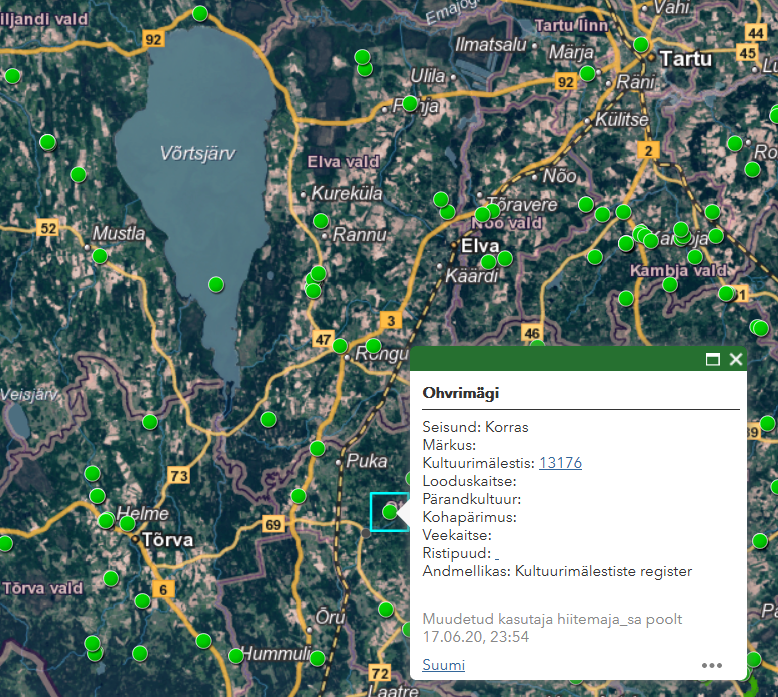
\includegraphics[width=0.45\linewidth]{C:/Users/a71386/Desktop/GeoHum/andres/geohumcourse/imgs/pringi1} 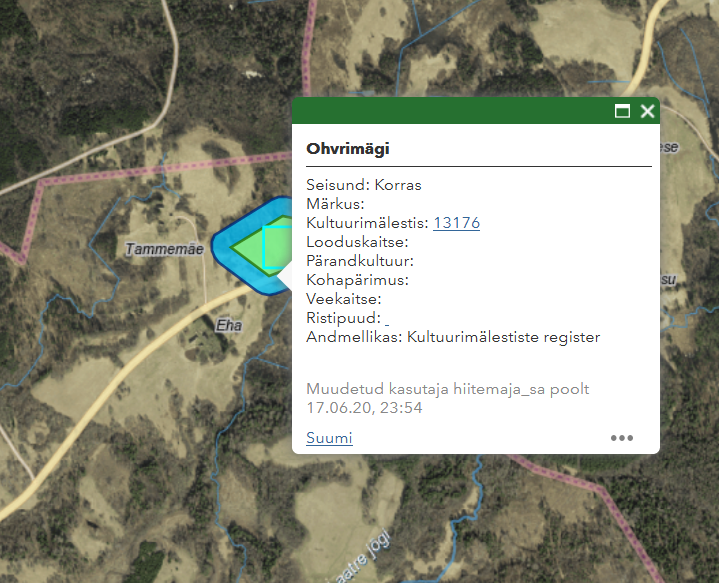
\includegraphics[width=0.45\linewidth]{C:/Users/a71386/Desktop/GeoHum/andres/geohumcourse/imgs/pringi2} 

}

\caption{[Pringi Ohvrimägi punktina ja polügoonina](https://hiitemaja.maps.arcgis.com/apps/webappviewer/index.html?id=db7d4fe754d245b9ac53f6d9a76e229e)}\label{fig:pringi1}
\end{figure}

\textbackslash begin\{figure\}

\{\centering 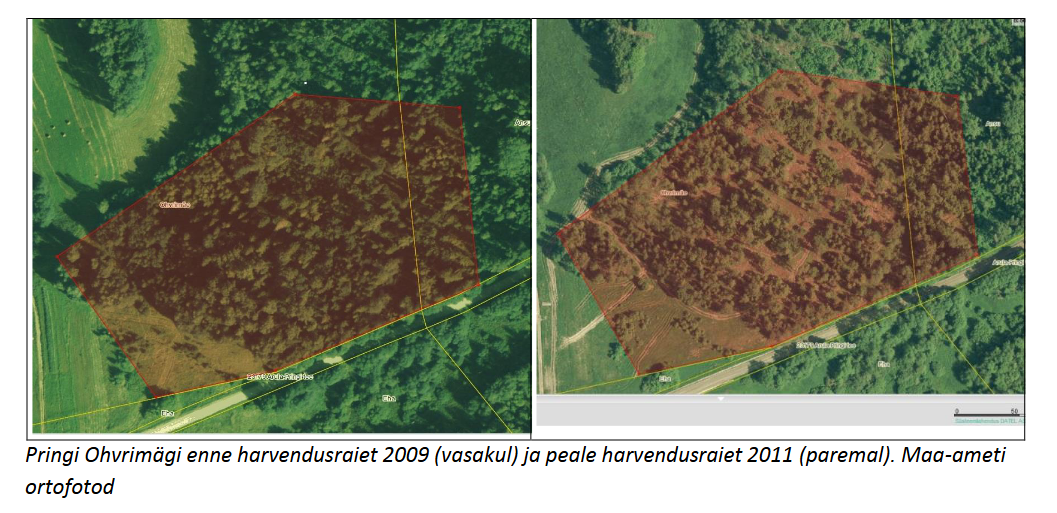
\includegraphics[width=1\linewidth]{C:/Users/a71386/Desktop/GeoHum/andres/geohumcourse/imgs/pringi3}

\}

\textbackslash caption\{\href{http://hiis.ee/files/ryystatud_pyhapaigad_2018.pdf}{Pringi Ohvrimäe raietööd}\}\label{fig:pringi3}
\textbackslash end\{figure\}

Vaatame natuke \href{http://orbis.stanford.edu/}{sellel lehel} ringi. Milliseid ruumiobjekte on kujutatud?

Vektorandmete struktuur võib olla väga erinev. Kõige lihtsamas struktuuris on iga objekt (punkt, joon või polügoon) kirjeldatud \emph{x}- ja \emph{y}-koordinaatide jada kaudu. See tähendab ka näiteks, et teineteisega külgnevad polügoonid on kirjeldatud eraldi joonelõikude kaudu, olgugi et neil on osa lõike ühised. Sellises struktuuris ei ole objektidevahelised suhted kuidagi kirjeldatud ning külgnemissuhe on implitseeritud ainult samasuguste koordinaatide kaudu.

Teine levinud viis andmeid struktureerida on kasutada \textbf{topoloogilisi suhteid}, mis kirjeldaksid ruumiobjektide paiknemissuhteid nii, et need mingite teisenduste (nt pööramise, suumimise, nihutamise) käigus ei muutuks. Näiteks külgnevate polügoonide puhul teab polügoonide ühine joonelõik, et tema parem pool kuulub ühte polügooni ja vasak pool teise ning kaob ära vajadus samu koordinaate kaks korda määrata.

\begin{figure}

{\centering 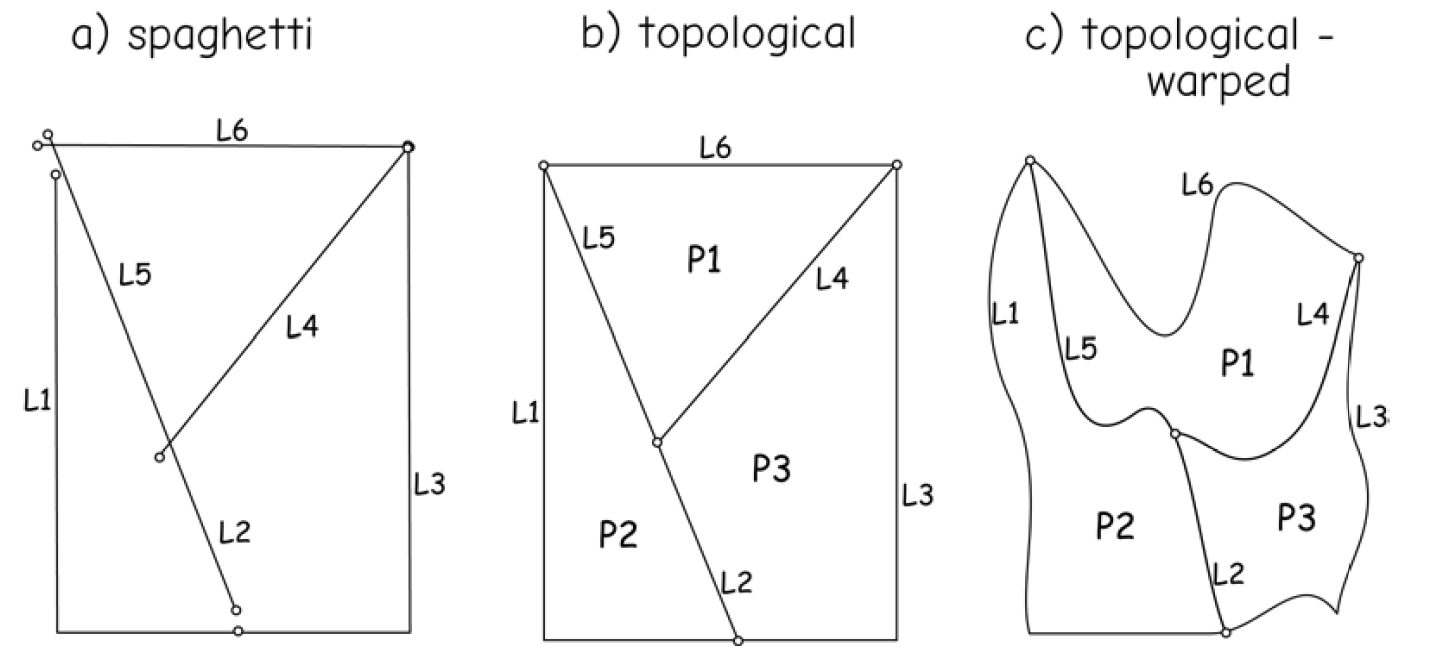
\includegraphics[width=1\linewidth]{C:/Users/a71386/Desktop/GeoHum/andres/geohumcourse/imgs/spaghetti_topological} 

}

\caption{Spagetistruktuur vs. topoloogiline struktuur [@Bolstad2016 : 48]}\label{fig:spaghetti-topological}
\end{figure}

Topoloogilised suhted on aluseks topoloogiareeglitele.

\begin{figure}
\centering
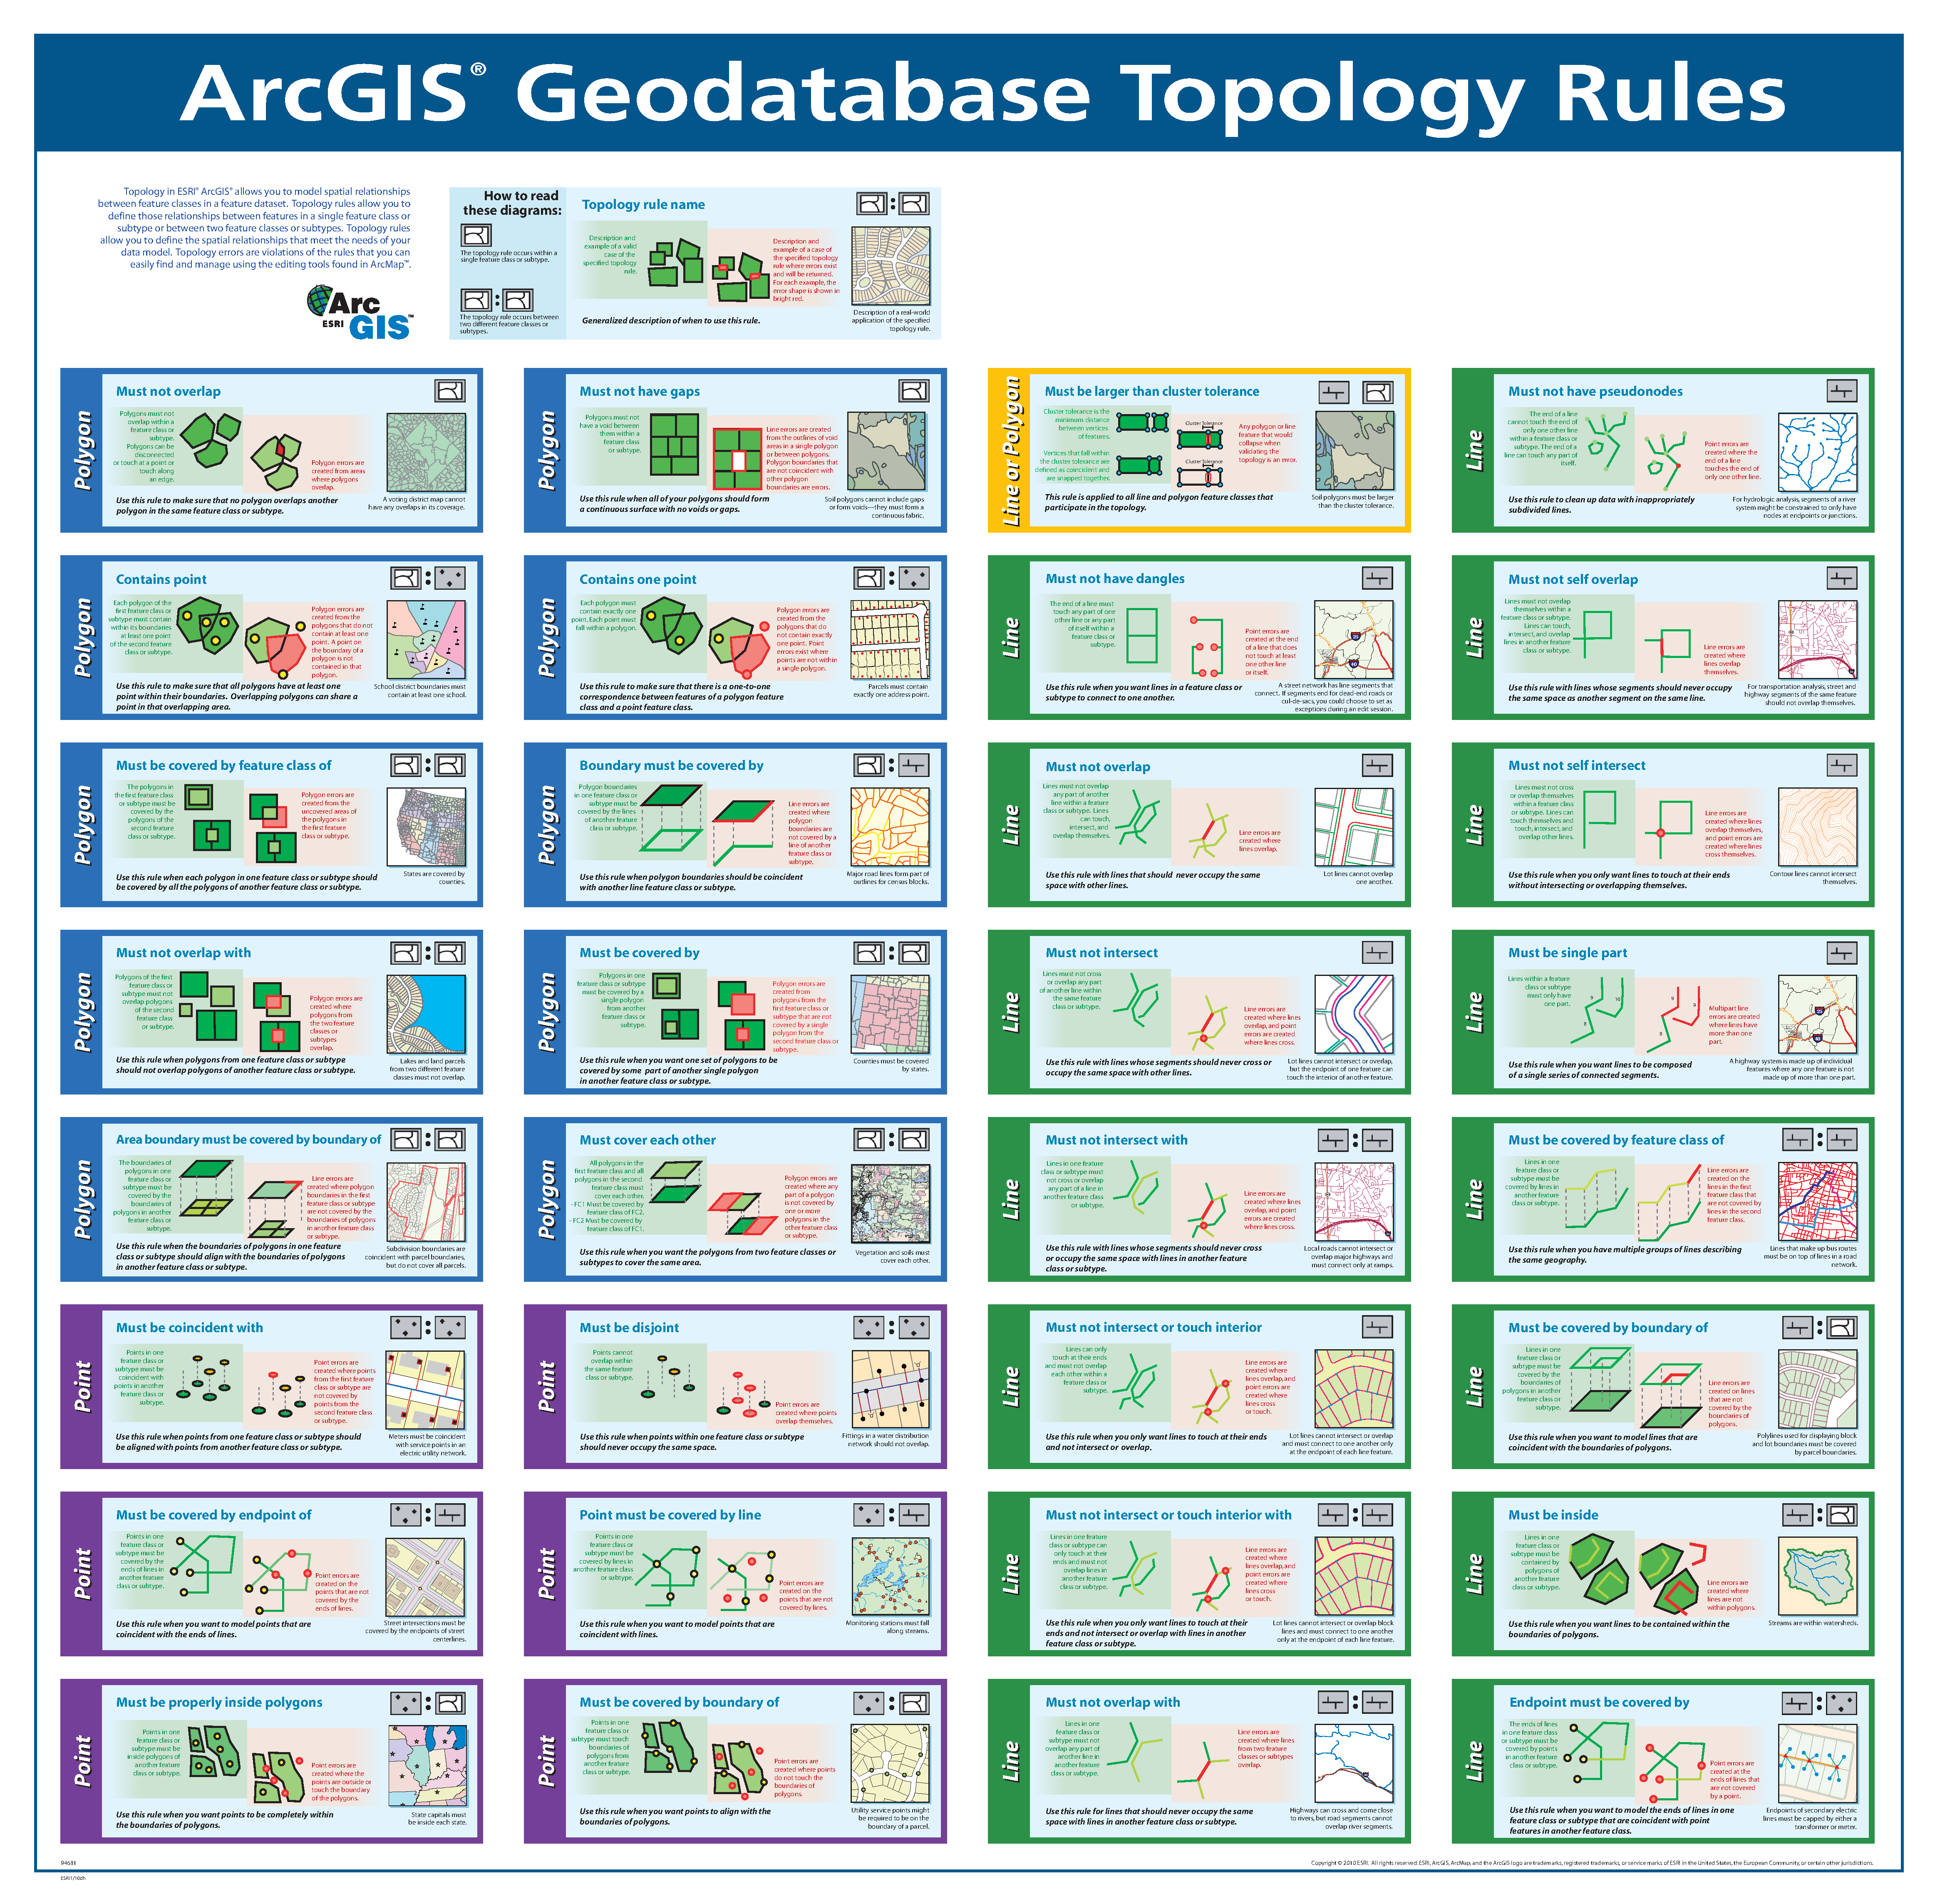
\includegraphics[width=1\textwidth,height=7.29167in]{http://resources.arcgis.com/en/help/main/10.2/01mm/pdf/topology_rules_poster.pdf}
\caption{Topoloogiareeglid ArcGISis}
\end{figure}

Topoloogilisi suhteid ja reegleid kasutatakse näiteks siis, kui tahetakse planeerida võimalikult kiiret teekonda ühest punktist teise või hoonestuse paiknemist, aga ka paljuks muuks. Pelgaks visualiseerimiseks pole aga topoloogilisi suhteid andmebaasis vaja defineerida.

Vektorandmeid hoitakse GISis enamasti kas SHP, GDB, TAB, DXF või VPF formaatides.

\hypertarget{rasterandmed}{%
\section{Rasterandmed}\label{rasterandmed}}

\textbf{Rastermudelit} kasutatakse eeskätt pidevate andmeobjektide (nn \emph{väljade}) kujutamiseks. Rastermudelis jagatakse ruum ühesuguste (kindla kujuga) osadega korrapäraseks võrguks ehk \emph{rastriks}, nii et igale rastri elemendile saab koordinaatide abil ühtmoodi viidata.

Rastermudel peaks olema tõenäoliselt juba tuttav, kui oled kokku puutunud näiteks digifotodega või muude digiteeritud piltidega. Formaadid, nagu JPEG, TIFF, GIF jm, põhinevad kõik rastermudelil. Samuti põhinevad rastertehnoloogial nt kõiksugu LCD-monitorid.

\begin{figure}

{\centering 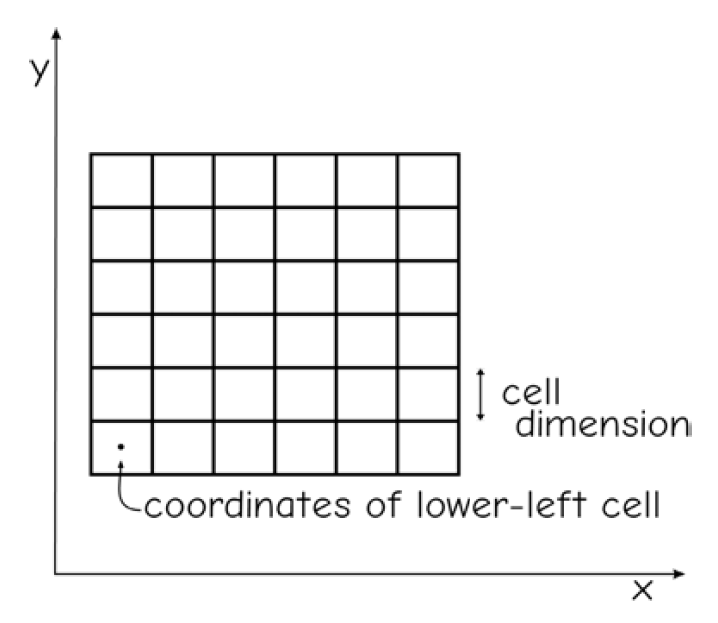
\includegraphics[width=1\linewidth]{C:/Users/a71386/Desktop/GeoHum/andres/geohumcourse/imgs/raster_model} 

}

\caption{Rastermudeli struktuur [@Bolstad2016 : 54]}\label{fig:raster}
\end{figure}

Rastri üht elementi nimetatakse tavaliselt \textbf{piksliks} (\emph{pixel} ehk \emph{picture element}). Pikslid võivad olla igasuguse kujuga, ent enamasti on need siiski ruudukujulised. Olgugi, et piksel on olemuselt alati kahemõõtmeline, on piksli koordinaatideks selle keskpunkti koordinaadid. Ühel pikslil on terves oma ulatuses üks väärtus (vastaval alal kõige tüüpilisem või keskmine väärtus), mis täpsustab näiteks selle piksli värvi ja/või heleduse ning iseloomustab selle kaudu piksliga piiratud alas asuva ruumilise nähtuse mingit omadust. Selline omadus võib olla nii pidev (nt kõrgusinfo, mingi keelelise konstruktsiooni suhteline kasutussagedus) kui ka diskreetne (nt konstruktsiooni \emph{A} vs.~konstruktsiooni \emph{B} kasutus).

See, kui täpselt rastermudel mingile reaalse maailma andmeobjekti kujule vastab, sõltub sellest, kui suured on ühe rastri elemendi ehk piksli mõõtmed ehk sellest, kui suur on \textbf{eraldusvõime/lahutusvõime}. Mida kõrgem on eraldusvõime, seda täpsem rastermudel on, ent seda suurem on ka rasterandmete faili suurus; mida madalam on eraldusvõime, seda enam infot läheb kaotsi. Efektiivseks eraldusvõime määramiseks tuleks arvesse võtta nii kaardi mõõtkava kui ka muude kaardistatavate andmete väikseimat ühikut.

\begin{figure}

{\centering 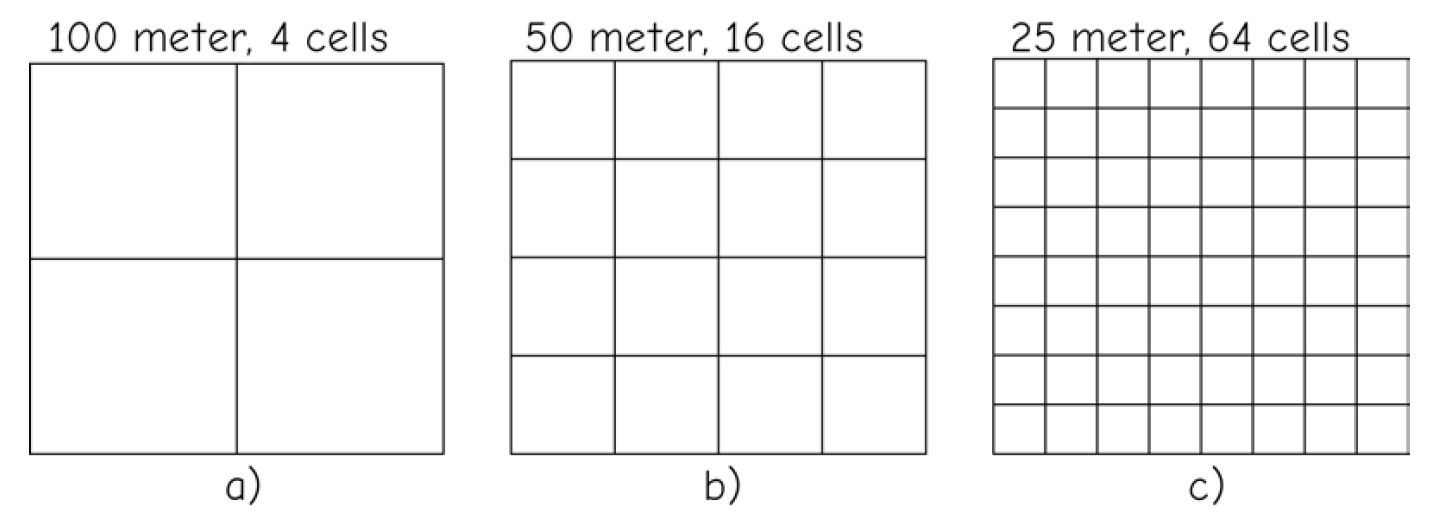
\includegraphics[width=1\linewidth]{C:/Users/a71386/Desktop/GeoHum/andres/geohumcourse/imgs/Bolstad2016_rasters} 

}

\caption{Rastri resolutsioon [@Bolstad2016 : 55]}\label{fig:unnamed-chunk-2}
\end{figure}

GISi seisukohast on eraldi liik rasterandmeid \textbf{satelliitpildid, aerofotod ja ortofotod}, mis pakuvad GISile olulist kontekstilist infot.
Satelliitide põhjal on võimalik kuvada suurt hulka maapinna omadusi ja protsesse. Aktiivsed satelliidid kasutavad kaugsensoreid, mis mõõdavad aega, mis kulub selleks, et sensorist edastatud signaal mingilt objektilt tagasi jõuaks. Passiivsete satelliitide sensorid kasutavad objektide kauguste arvutamiseks looduslikest allikatest (nt päikeselt) peegeldunud või kiiratud elektromagnetkiirgust. Erinevad satelliidid annavad siinjuures erineva kvaliteediga pilte.

\textbackslash begin\{figure\}

\{\centering 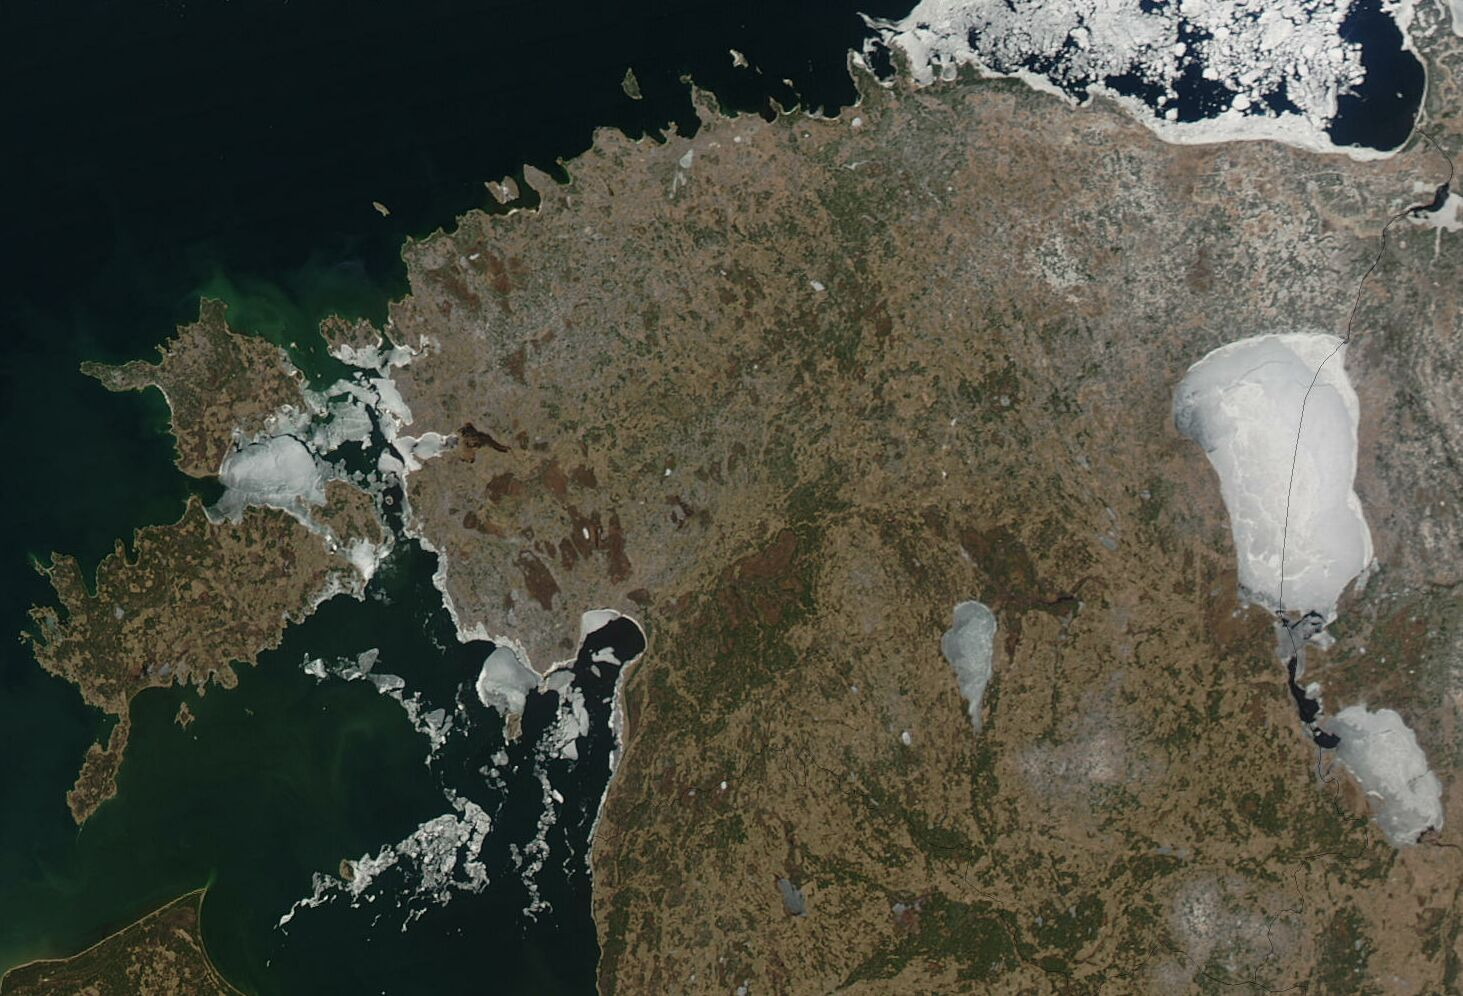
\includegraphics[width=1\linewidth]{C:/Users/a71386/Desktop/GeoHum/andres/geohumcourse/imgs/satelliit}

\}

\textbackslash caption\{Eesti satelliitpilt (\href{https://commons.wikimedia.org/wiki/File:Satellite_image_of_Estonia_in_April_2004.jpg}{allikas})\}\label{fig:satelliit}
\textbackslash end\{figure\}

Vaata värskemaid NASA satelliitpilte \href{https://wvs.earthdata.nasa.gov/?COORDINATES=55.0171,17.8288,61.4922,35.0957}{siit}.

Aerofotosid saab teha näiteks õhupallist, kopterist või lennukist ning lisaks nähtavale visuaalsele infole saab vastavate sensorite abil salvestada ka nt ultraviolett- või infrapunakiirgust. Aerofotod võivad oma läätse tõttu olla servadest moonutatud ning samuti võivad moonutatud olla maapinnast kõrgel olevad objektid (nt tornid, korstnad, tipud). Ortofotod on geomeetriliselt parandatud aerofotod.

\begin{figure}

{\centering 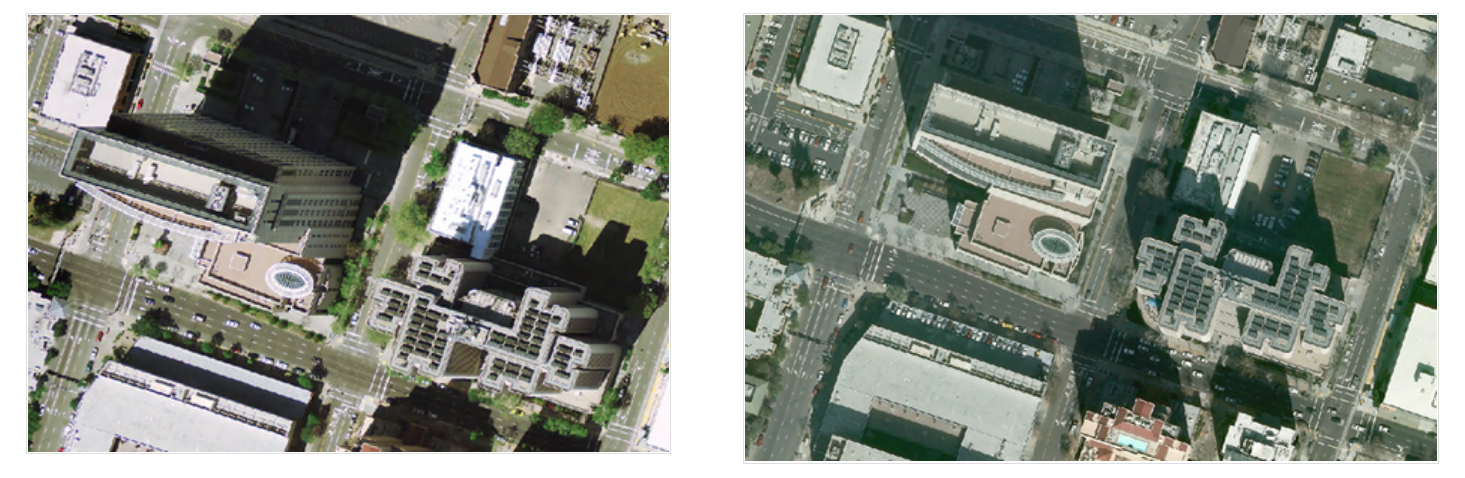
\includegraphics[width=1\linewidth]{C:/Users/a71386/Desktop/GeoHum/andres/geohumcourse/imgs/aerofoto_ortofoto} 

}

\caption{Aerofotod vs. ortofotod ([allikas](https://opengeospatial.weebly.com/31-remote-sensing-platforms.html))}\label{fig:aero-orto}
\end{figure}

Rasterpildid sobivad hästi illustratsiooniks või kaardi aluskihiks, ent halvemini kartograafiliseks modelleerimiseks.

Rastreid võib aga saada ka \textbf{vektorandmete teisendamisel või interpoleerimisel rasterkujule}. Sellisel juhul võib pidada üheks rastri elemendiks nn \textbf{rakslit} ning selle väärtus viitab enamasti mingi ruumiobjekti ID-le või mingi atribuudi väärtusele.

\begin{figure}

{\centering 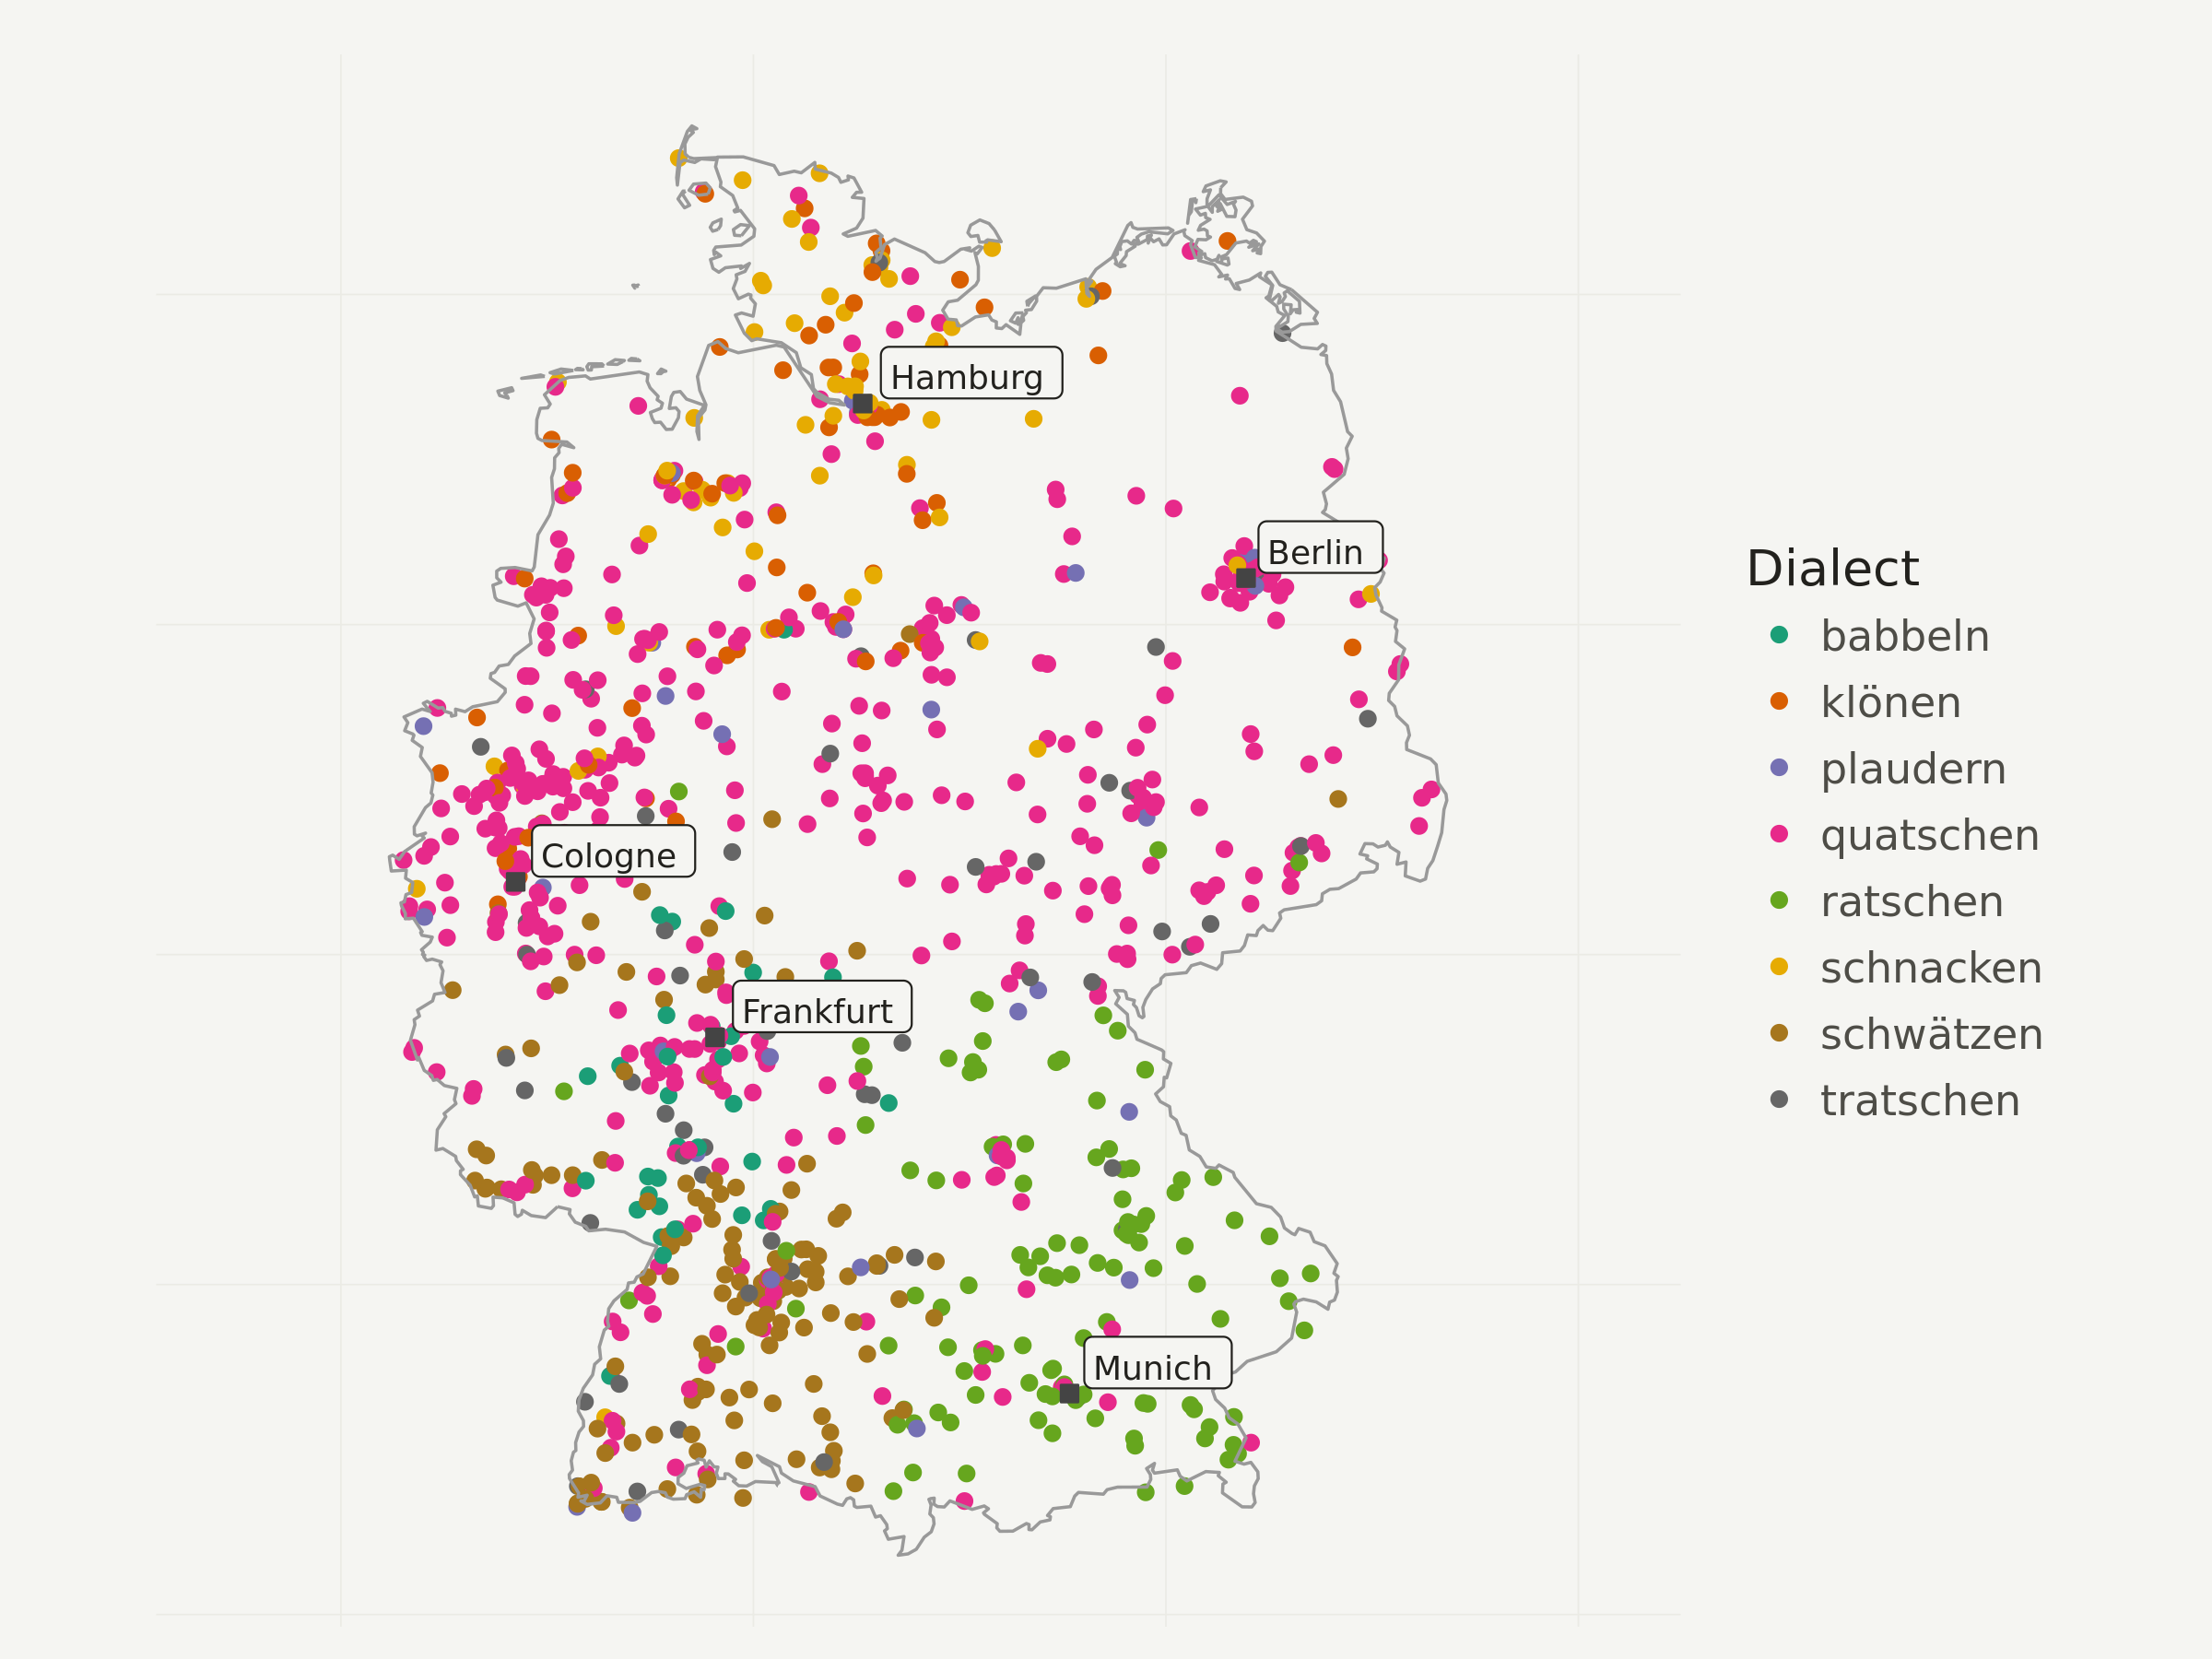
\includegraphics[width=0.45\linewidth]{C:/Users/a71386/Desktop/GeoHum/andres/geohumcourse/imgs/chat1_points} 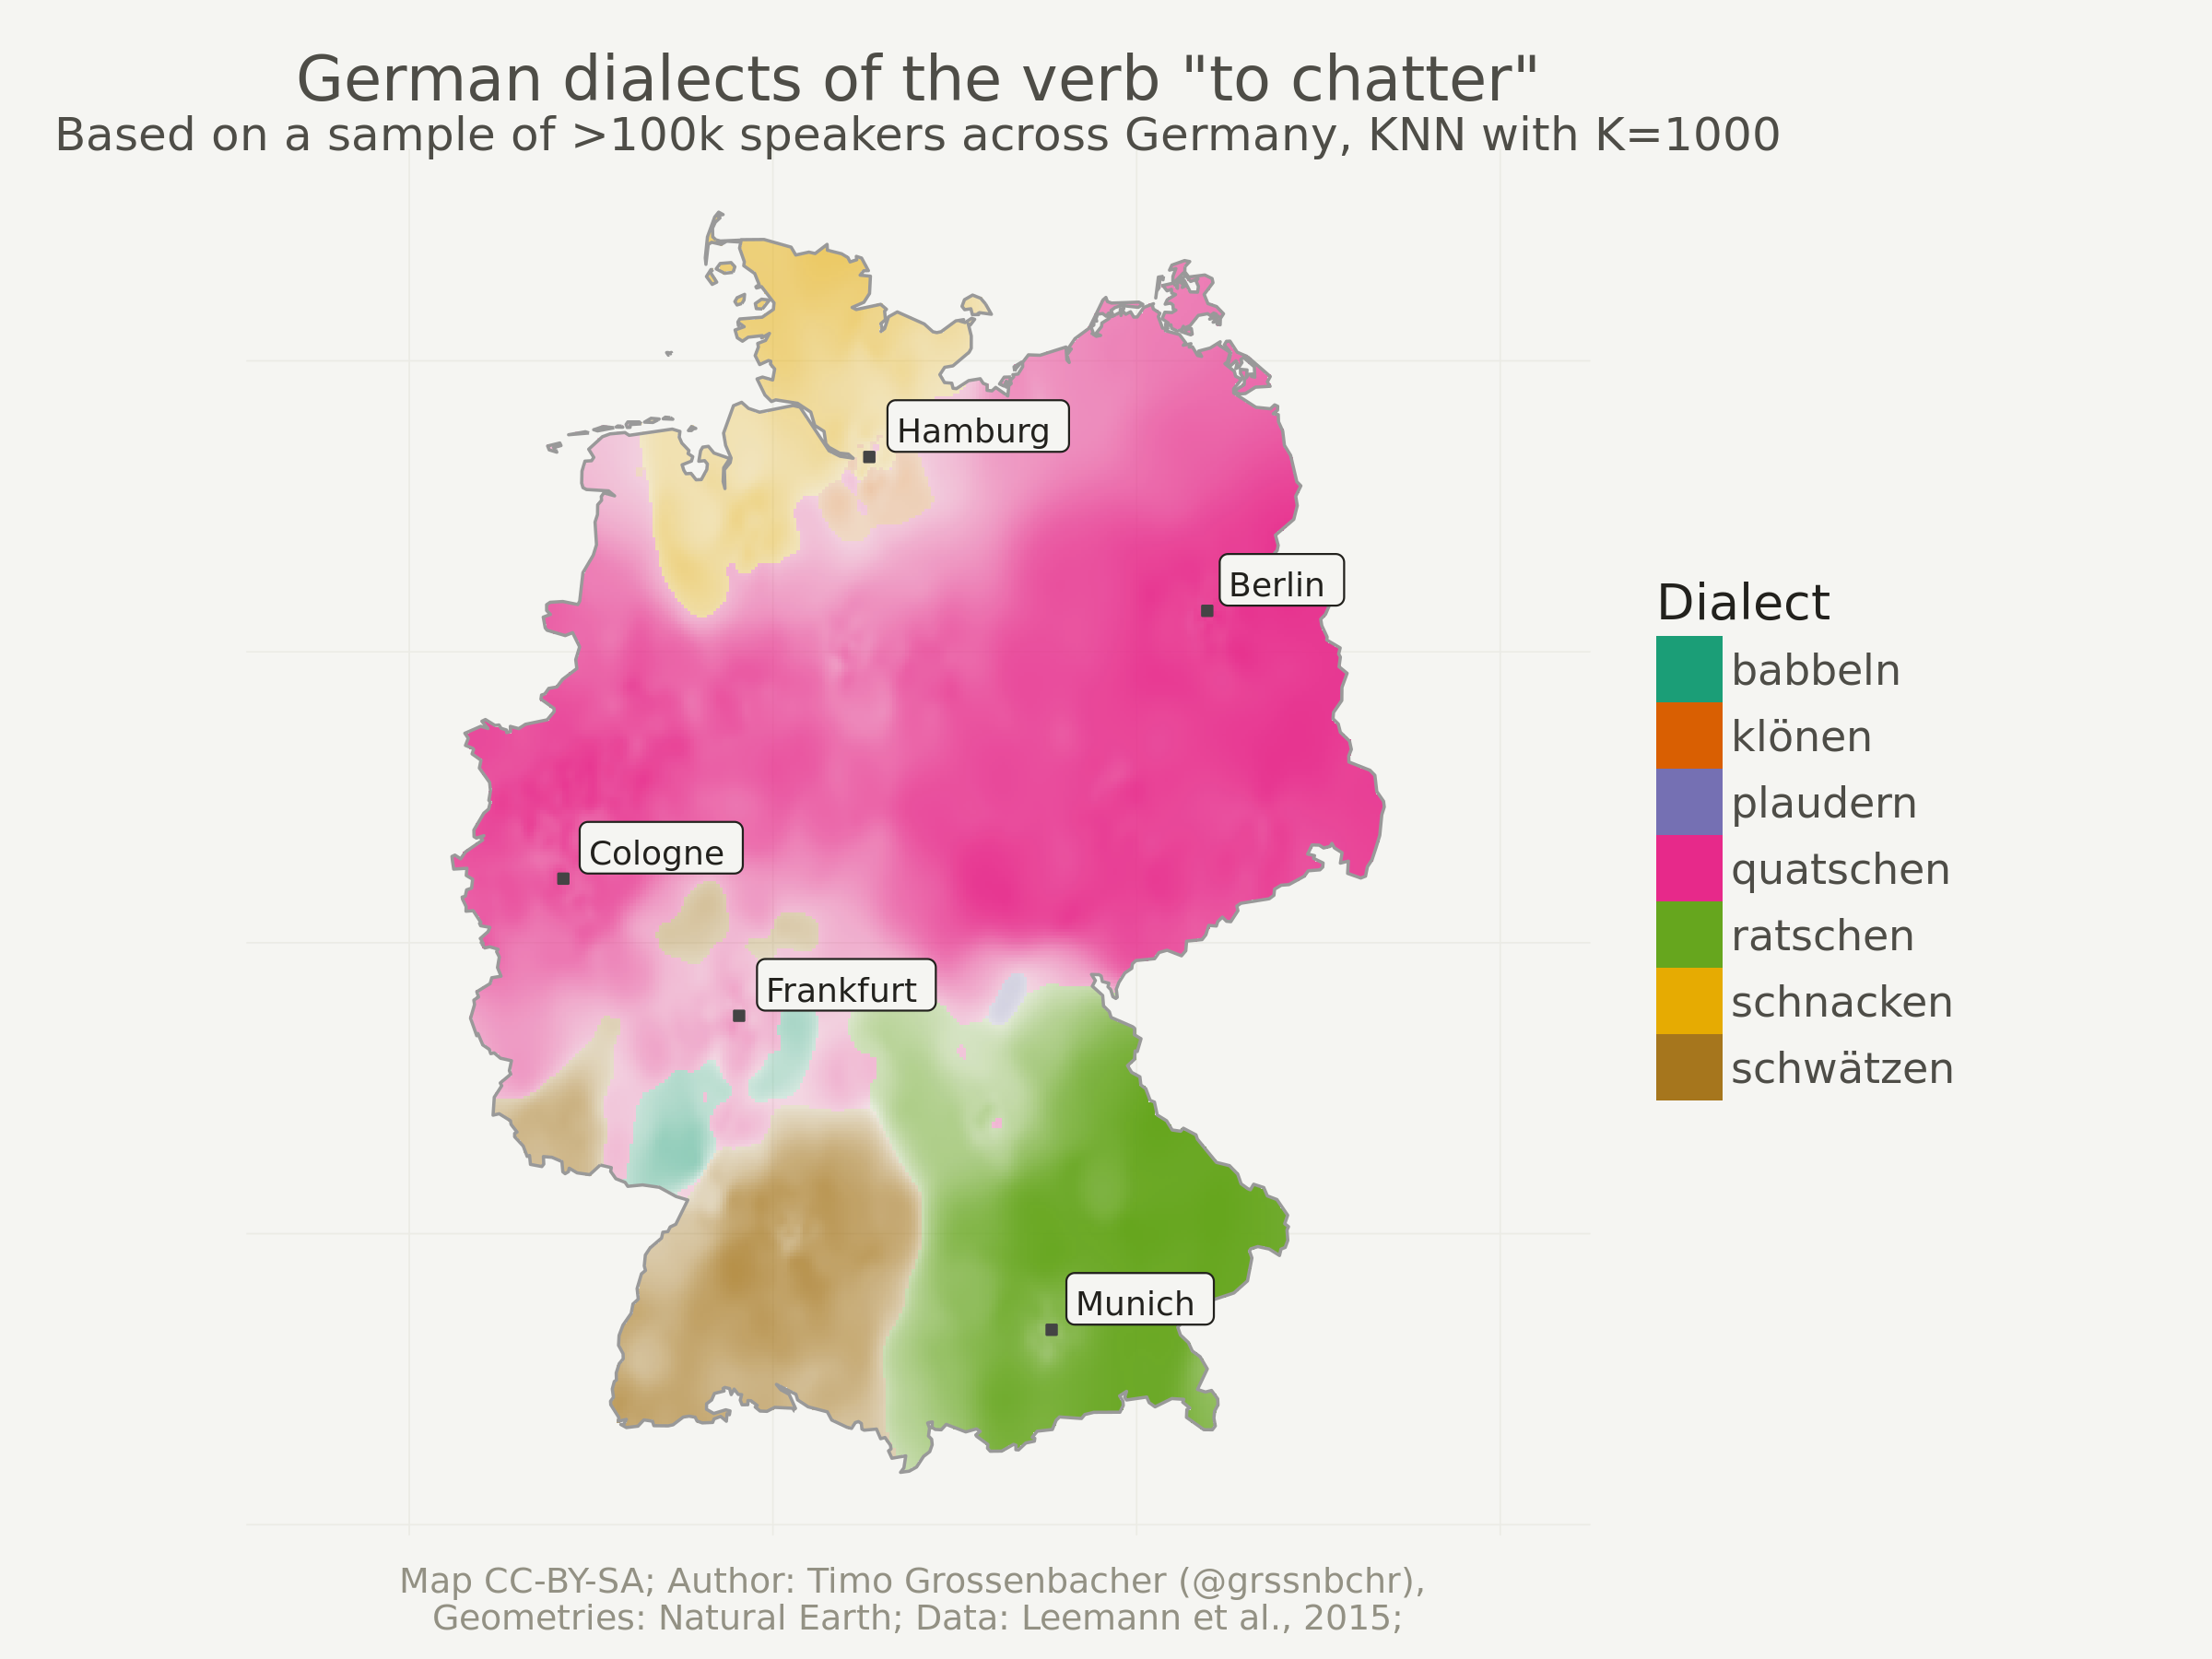
\includegraphics[width=0.45\linewidth]{C:/Users/a71386/Desktop/GeoHum/andres/geohumcourse/imgs/chat2_raster} 

}

\caption{Vektorandmetest rasterandmeteni, vt lähemalt [siit](https://timogrossenbacher.ch/2018/03/categorical-spatial-interpolation-with-r/)}\label{fig:german-dialects}
\end{figure}

Rasterandmete levinumad formaadid on näiteks JPEG, PNG, TIFF, BMP, GIF.

\hypertarget{vektor-vs.-raster}{%
\section{Vektor vs.~raster}\label{vektor-vs.-raster}}

Vektorandmed

Rasterandmed

andmestruktuur võib olla keerukas

andmestruktuur on lihtne

vähem mahukad

võivad olla väga mahukad

sobivad ruumiobjektide piiritlemiseks või nende asukoha keskpunktide määramiseks

sobivad paremini mingil alal esineva (pideva) nähtuse iseloomustamiseks

sobivad paremini inimtegevuse kujutamise jaoks

sobivad paremini keskkonna- või loodusnähtuste jaoks

sobivad paremini konkreetsetele nähtustele paljude atribuutidega

sobivad paremini komplekssetele nähtustele väheste atribuutidega

sobivad paremini täpsete, konkreetsete andmetega

sobivad paremini ebatäpsete/puudulike või üldistavate andmetega

võib arvestada ka topoloogilisi suhteid

enamasti objektidevahelisi suhteid ei arvesta

on vähem tundlikud projektsiooni muutmisele

võivad olla väga tundlikud projektsiooni muutmisele

kaardid on visuaalselt ilusamad

kaardid suhteliselt robustsed

\textbf{Mõttepaus}:

\begin{itemize}
\tightlist
\item
  Kumba mudelit kasutaksid riigimaanteede kaardistamiseks? Miks?\\
\item
  Kumba mudelit kasutaksid rahvastikutiheduse mudeldamiseks? Miks?\\
\item
  Millisel kujul saaksid kujutada enda uurimisainest?
\end{itemize}

Paljud tänapäeva GIS-tehnoloogiad võimaldavad kasutada mõlemat mudelit paralleelselt. Näiteks digitaalsed maastikumudelid kuvavad sageli rasterandmete abil mingi piirkonna reljeefi või maakasutust, punktide abil huvipakkuvaid hooneid, joonte abil jõgesid ja teid ning polügoonide abil haldusjaotust. Sealjuures võib otsustada, kas kuvada näiteks kirikud, haiglad ja haridusasutused eraldi kihtidel või ühe kihina, milles sisaldub hoone funktsiooni määrav atribuut.

\begin{figure}
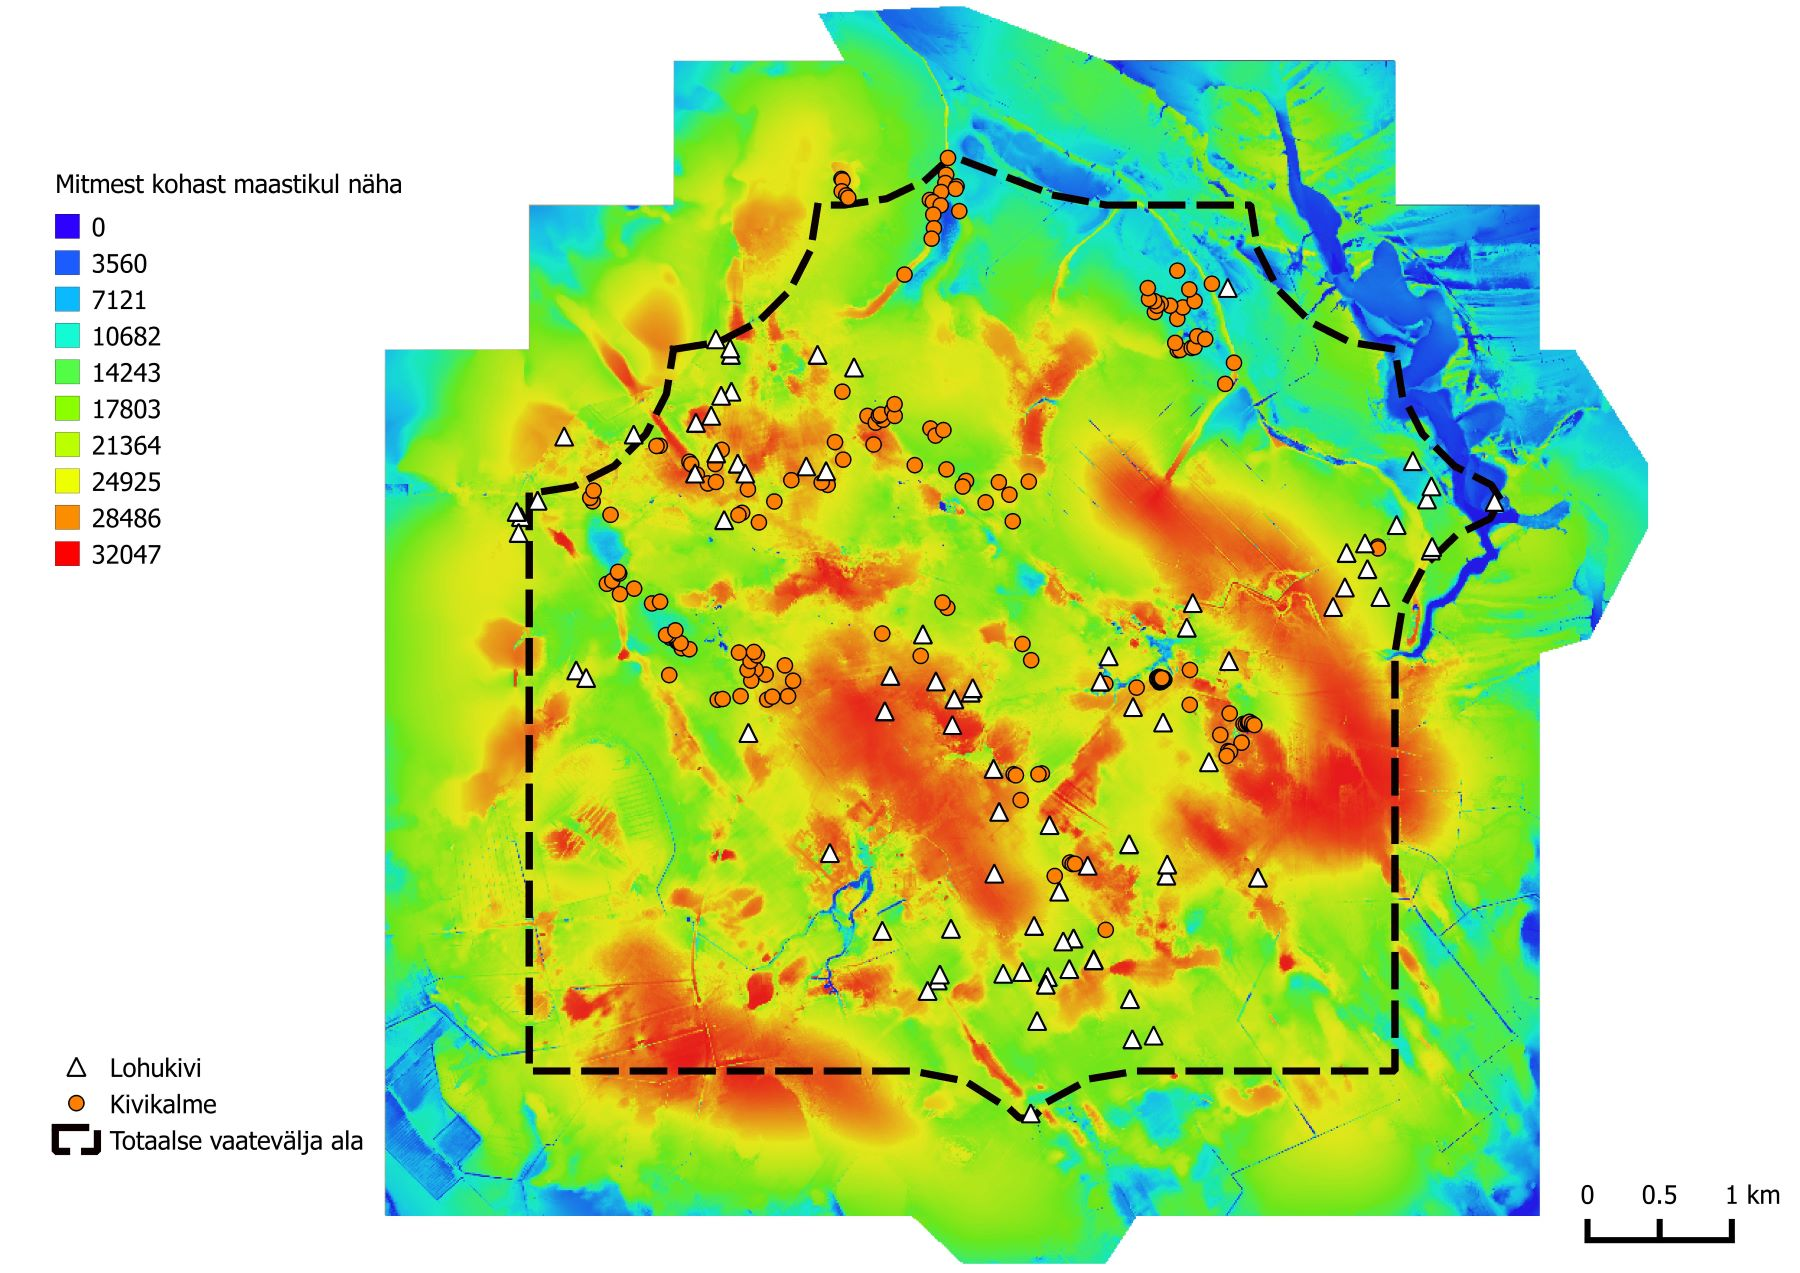
\includegraphics[width=1\linewidth]{C:/Users/a71386/Desktop/GeoHum/andres/geohumcourse/imgs/arheo_example_kimber_lohukivid_totalviewshed} \caption{Maastiku nähtavuse analüüsimine [@Kimber2016, jn 5]}\label{fig:arheo-ex}
\end{figure}

Samuti võib üht ja sama nähtust kuvada erinevat moodi.

\begin{figure}
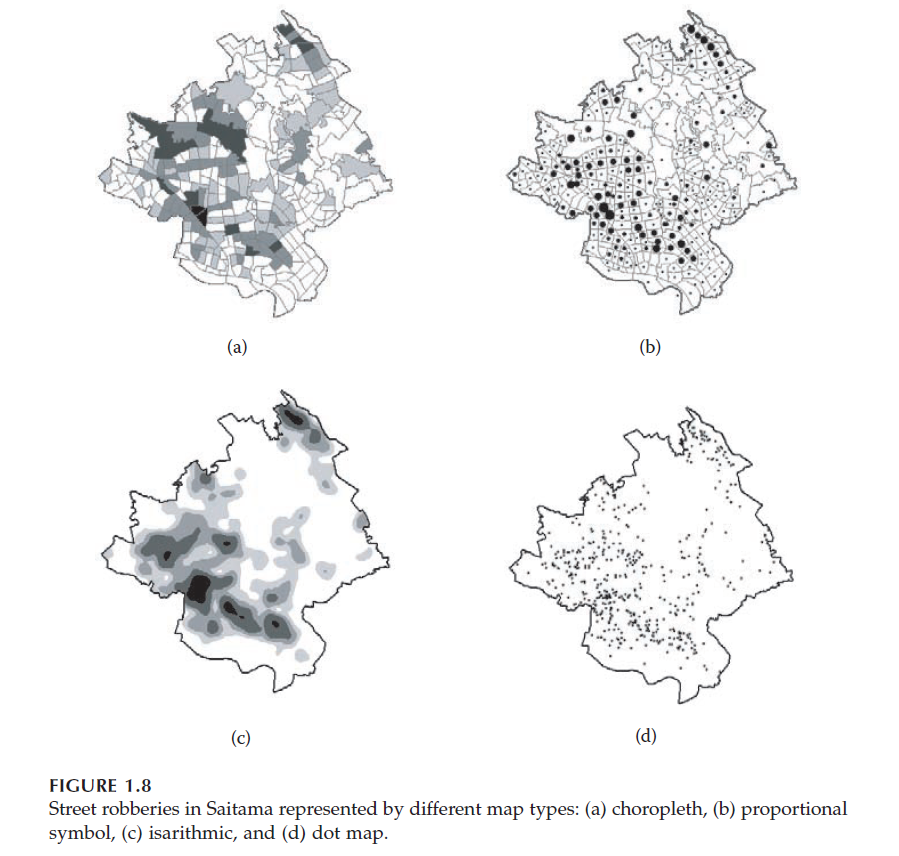
\includegraphics[width=1\linewidth]{C:/Users/a71386/Desktop/GeoHum/andres/geohumcourse/imgs/okabe_2006} \caption{Tänavaröövid Saitamas [@Okabe2006 : 8]}\label{fig:unnamed-chunk-3}
\end{figure}

Vaata natuke \href{http://blog.ut.ee/30-maps-of-estonia-in-30-days/}{siin} ringi. Kas saad aru, millist tüüpi mudeleid on kasutatud?

\hypertarget{uxfclesanne}{%
\section{Ülesanne}\label{uxfclesanne}}

Kujuta ette, et Google Mapsi ei ole veel leiutatud ja paberkaardid on väga kallid, aga sulle on Tartusse külla tulnud sõber / perekonnaliige / tuttav / välismaa sõber, kes ei ole siin kunagi varem käinud. Joonista tema jaoks paberile Tartu kesklinna kaart ning lisa kaardile juurde, kellele kaart on mõeldud.

\hypertarget{juxe4rgmisel-korral-1}{%
\section{Järgmisel korral}\label{juxe4rgmisel-korral-1}}

Neljapäeval räägime lähemalt kaartidest ja nende omadustest ning uurime vabavaraliste kaardirakenduste võimalusi ja piiranguid.

\hypertarget{kirjandus-1}{%
\section{Kirjandus}\label{kirjandus-1}}

\hypertarget{kaardirakendused}{%
\chapter{Kaardirakendused}\label{kaardirakendused}}

Enne, kui hakkame rääkima sellest, kuidas juba olemasolevate veebirakendustega kaarte koostada, peame lühidalt ja sissejuhatavalt rääkima veidi sellest, \textbf{mis kaart on}.

\hypertarget{kaart}{%
\section{Kaart}\label{kaart}}

Kaart on kitsamas tähenduses geograafilise informatsiooni visuaalne esitusviis. GISis on kaardid nii sisendiks kui ka väljundiks. Laiemas tähenduses võime kaardiks pidada mis tahes esitust maailmast.

\begin{figure}

{\centering 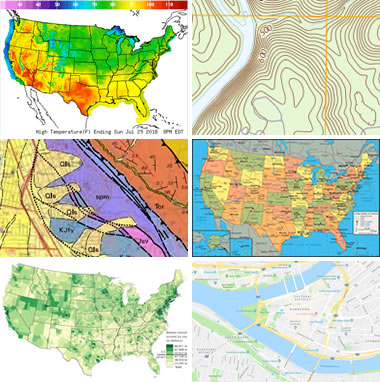
\includegraphics[width=1\linewidth,height=1\textheight]{C:/Users/a71386/Desktop/GeoHum/andres/geohumcourse/imgs/types-of-maps} 

}

\caption{[Erinevaid kaarte](https://geology.com/maps/types-of-maps/)}\label{fig:map-types}
\end{figure}

\begin{figure}

{\centering 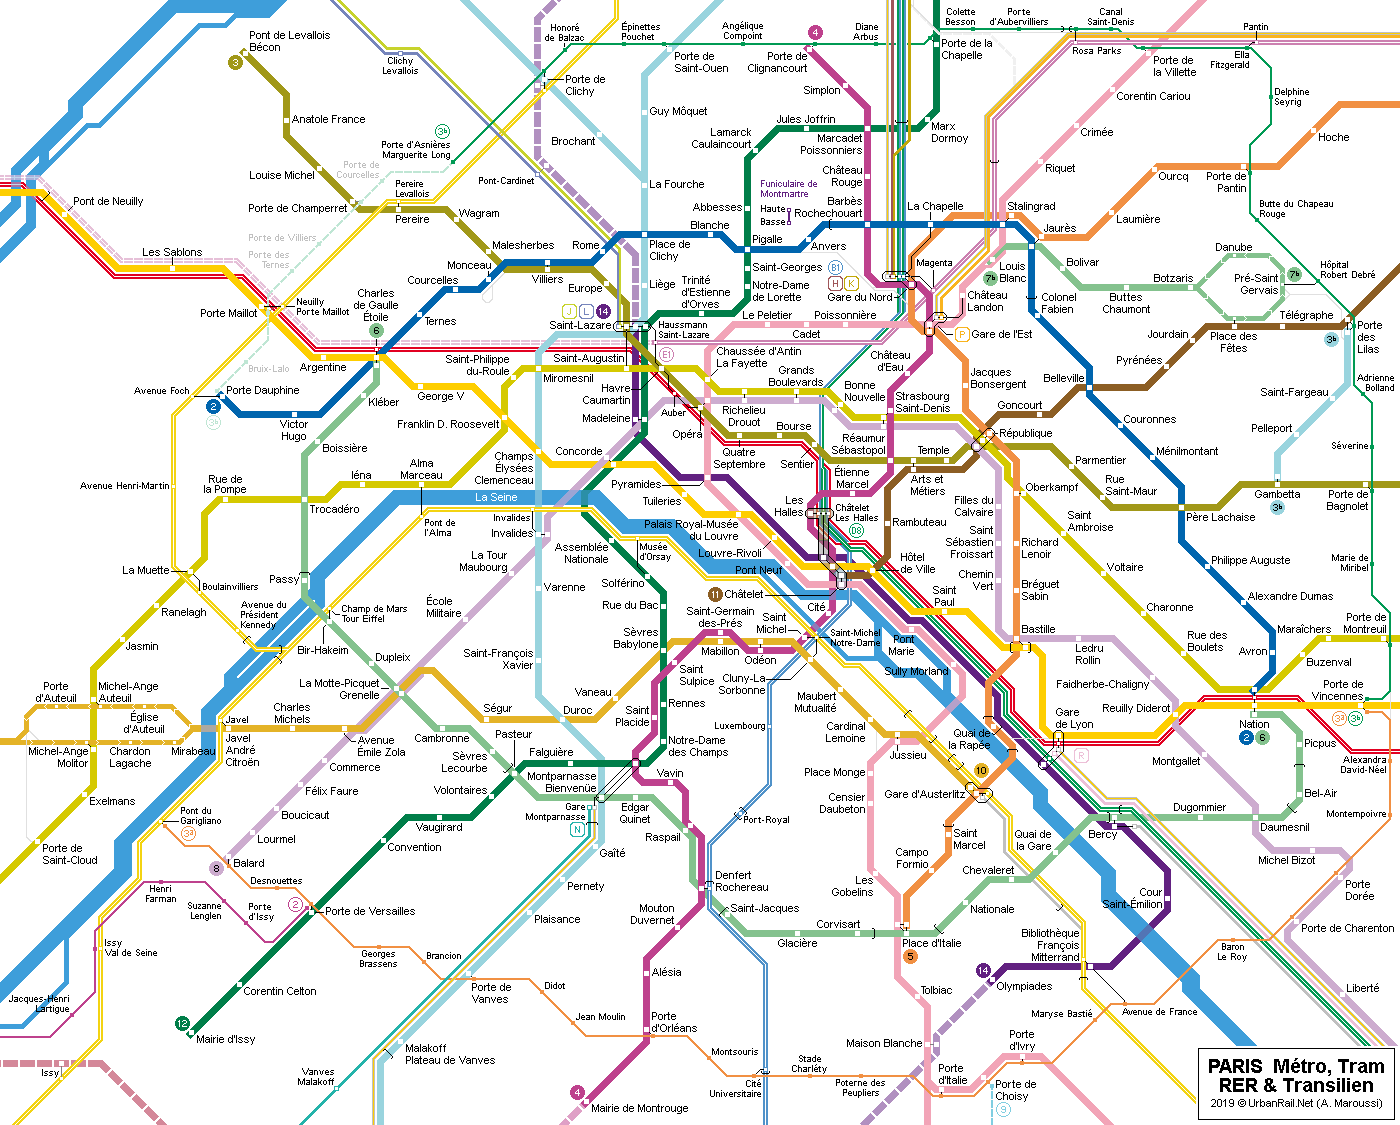
\includegraphics[width=1\linewidth,height=1\textheight]{C:/Users/a71386/Desktop/GeoHum/andres/geohumcourse/imgs/paris-metro} 

}

\caption{[Pariisi metrookaart](http://www.urbanrail.net/eu/fr/paris/paris.htm/)}(\#fig:paris metro)
\end{figure}

\begin{figure}

{\centering 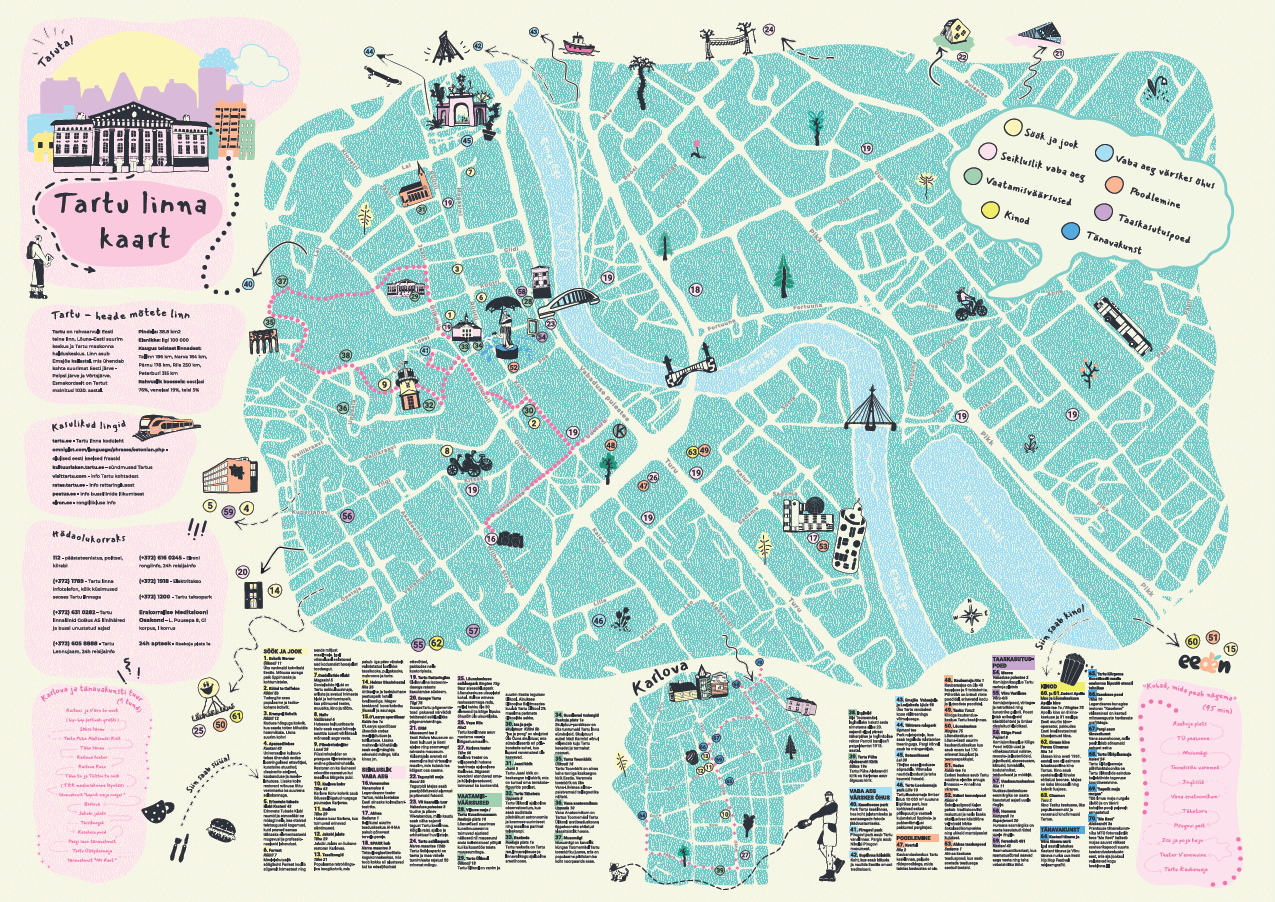
\includegraphics[width=1\linewidth,height=1\textheight]{C:/Users/a71386/Desktop/GeoHum/andres/geohumcourse/imgs/tartu_kaart_noored} 

}

\caption{[Tartu kaart](https://tntk.tartu.ee/tartu-noorsootoo-keskus/reveal-youropean-cultural-heritage-enrich/tartu-kaart/)}\label{fig:noored}
\end{figure}

Kaarti tehes peame alati esmalt läbi mõtlema, mis on kaardi tegemise eesmärk ning kes on kaardi lõppkasutaja. Seejärel tuleb mõelda, mida ja mis kujul reaalsest maailmast esitame ning kui täpne peab esitus olema. Lõpuks tuleb mõelda ka tehnilistele aspektidele: mis formaadis andmed meil on kasutada, mis formaadis need andmed peavad olema kaardi tegemiseks ning mis formaadis tuleb kaart ise.

GISis võime infot esitada kaardikihtidena, kusjuures ühel kihil esitatakse nähtusi, mis omavad \textbf{ühesugust ruumiobjekti tüüpi}. See tähendab, et samal kihil ei tohiks esitada näiteks jõgesid (tüüpiliselt avatud jooned) ja ehitisi (tüüpiliselt suletud jooned ehk polügoonid). Küll aga võime soovi korral esitada samal kihil näiteks kive, restorane ja kogumispunkte, mis küll olemuslikult on erinevast klassist, aga geomeetriliselt esitatavad sama tüüpi ruumiobjekti (punkti) abil. Üldiselt on tavaks esitada ühel kaardikihil siiski ka temaatiliselt sarnaseid objekte.

Üha rohkem puutume tänapäeval paberkaartide asemel kokku digitaalkaartidega. Ehkki mõlemal juhul näeme kaardil seda infot, mida kaardi tegija soovib edastada, ning sellisel kujul, nagu tema vajalikuks peab, on paber- ja digitaalkaartidel olulisi erinevusi.

\begin{figure}

{\centering 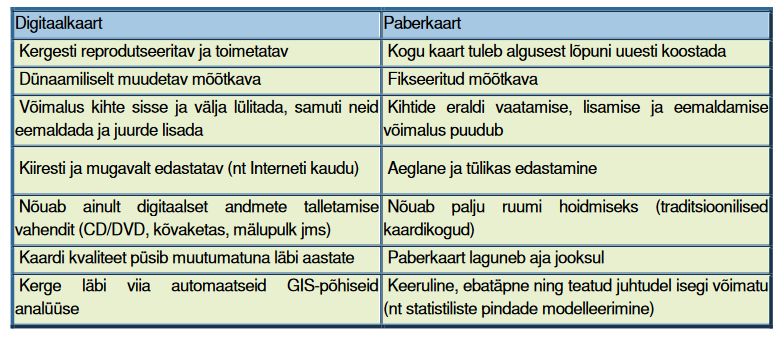
\includegraphics[width=1\linewidth]{C:/Users/a71386/Desktop/GeoHum/andres/geohumcourse/imgs/digitaal_paberkaart} 

}

\caption{Digitaal- vs. paberkaart [@Suurna&Sisas2010 : 26]}\label{fig:paber-digi}
\end{figure}

Kaartidel edastatakse mingit objekti või nähtust kirjeldavat informatsiooni hästi eristuvate ja loetavate leppemärkide, värvitoonide ja kirjade abil. Kaardil on aga veel mitmeid komponente, näiteks mõõtkava, suunaviit jm.

\begin{figure}

{\centering 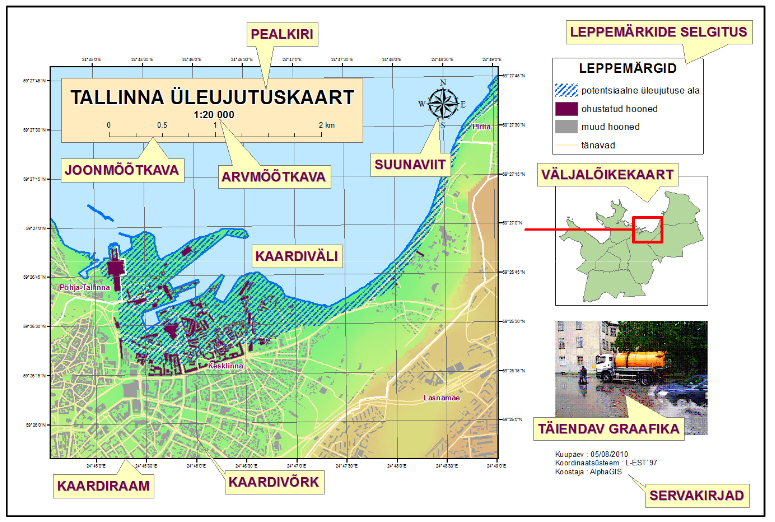
\includegraphics[width=1\linewidth]{C:/Users/a71386/Desktop/GeoHum/andres/geohumcourse/imgs/kaardi_komponendid} 

}

\caption{Kaardi komponendid [@Suurna&Sisas2010 : 33]}\label{fig:kaardi-komponendid}
\end{figure}

Kaardi \textbf{mõõtkava} näitab, kui palju reaalset objekti on vähendatud. Tavaliselt väljendatakse mõõtkava murdosa või suhtena, mis seob kaardil esitatud mingi pikkusega joonlõigu sama joonlõiguga maapinnal. Näiteks mõõtkava 1:20000 või 1/20000 näitab, et 1 ühik kaardil vastab 20000 samale ühikule reaalses maailmas. Kui ühik on cm, siis esitab 1 cm kaardil 20000 cm ehk 200 m maapinnal. Digitaalsetel kaartidel esitatakse mõõtkava sageli dünaamiliselt, mis tähendab, et mõõtkava saab sisse või välja suumides muuta. Samuti on tüüpiline mõõtkava esitamine mitte arvmõõtkavana, vaid visuaalselt: mingile ekraanil määratletud joonlõigule vastab tegelikkuses kindel vahemaa maapinnal, ent me ei pruugi täpselt näha, kui pika joonlõiguga on ekraanil tegemist.

Kui liigume suurelt mõõtkavalt väiksemale, peame andmeid loetavuse huvides üldistama ning valima, mida ja mis detailsusastmega esitada. Üldistada võib lihtsustades, siludes, ühendades jne.

\hypertarget{htmlwidget-ad6b0a4b17cf482b4af0}{}
\begin{leaflet}

\end{leaflet}

Kaartide kujunduslikest komponentidest räägime lähemalt siis, kui ise QGISis kaarte tegema hakkame, ent üldiselt tuleks kaartide kujunduses silmas pidada lihtsust ja arusaadavust. See tähendab, et kujundid, sümbolid, värvid jm peaksid olema kujutatava nähtusega kergesti seostatavad. Muidugi võib kaarti käsitleda ka kui omalaadi kunstiteost, mispuhul kokkuleppelised ja harjumuspärased kujutusviisid võivad jääda tagaplaanile.

\hypertarget{koordinaatsuxfcsteemid-ja-projektsioonid}{%
\subsection{Koordinaatsüsteemid ja projektsioonid}\label{koordinaatsuxfcsteemid-ja-projektsioonid}}

Ruumiandmed on alati seotud mingi kohaga. Maakera on kolmemõõtmeline ja põhimõtteliselt võiksime üsna hästi kasutada objektide asukoha ja omaduste kujutamiseks gloobust. See aga ei ole sageli kuigi praktiline. Kaardil, mis on märksa praktilisem visualiseerimisvahend, on üldjuhul aga ainult kaks mõõdet. Kuidas siis kolmemõõtmelist ning ebakorrapärast kujundit kujutada kahemõõtmelise ja korrapärase meediumi kaudu ning kuidas paigutada reaalse maailma objekte ja alasid nii, et saaksime kaardi põhjal öelda, kus need maakeral asuvad?

Esmalt tuleb objektid ja nähtused siduda mingite koordinaatidega. \textbf{Koordinaadid} on arvud, mis määravad punkti asendi tasandil või ruumis ning \textbf{koordinaatsüsteem} vastavalt teatud reeglitel põhinev raamistik, mida nende arvude määramiseks kahe- või kolmemõõtmelises ruumis kasutatakse. Ühtse koordinaatsüsteemi abil on võimalik siduda ja koos esitada erinevaid andmeid, ent kui tahame määrata koordinaate maapinnal, siis koordinaatsüsteemist üksi ei piisa. Vaja on siduda see ka Maa kui füüsilise keha ja selle kujuga.

Maa üldist kuju kirjeldab geodeetiline referentssüsteem ehk \textbf{daatum}, mis esitab Maa matemaatilise mudeli nii, et see vastaks võimalikult hästi Maa tegelikule kujule, sageli kui pöördellipsoidi või sferoidi. Erinevate ellipsoidide mõõtmed võivad pisut erineda (nt nende pooltelgede pikkused või ellipsoidi lapikus), sest Maa tegelik füüsiline kuju (geoid) on ellipsoidist märksa keerulisem. Nõnda sobivad mõned \textbf{lokaalsed} daatumid, mis ei ole tingimata seotud Maa keskpunktiga, väikesele maa-alale paremini, sest järgivad selles konkreetses kohas paremini Maa tegelikku kuju, ent ei ole jällegi hästi kasutatavad teistes kohtades.
Eestis kasutatakse tänapäeval \textbf{globaalset} geotsentrilist ellipsoidi \textbf{GRS80}, mis on praktiliselt identne palju laialdasemalt kasutusel oleva globaalse \textbf{WGS84} ellipsoidiga.

\begin{figure}

{\centering 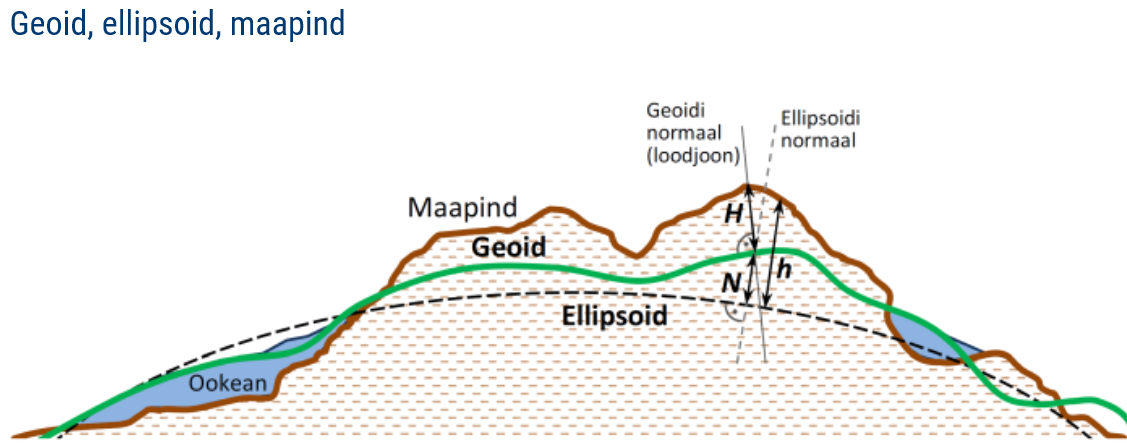
\includegraphics[width=15.65in]{C:/Users/a71386/Desktop/GeoHum/andres/geohumcourse/imgs/geoid_ellipsoid_maapind} 

}

\caption{Geoid, ellipsoid ja maapind (allikas: [Maa-amet](https://geoportaal.maaamet.ee/est/Ruumiandmed/Geodeetilised-andmed/Geodeetilised-vorgud/Geoid-p287.html))}\label{fig:geoid-ellipsoid}
\end{figure}

\begin{figure}

{\centering 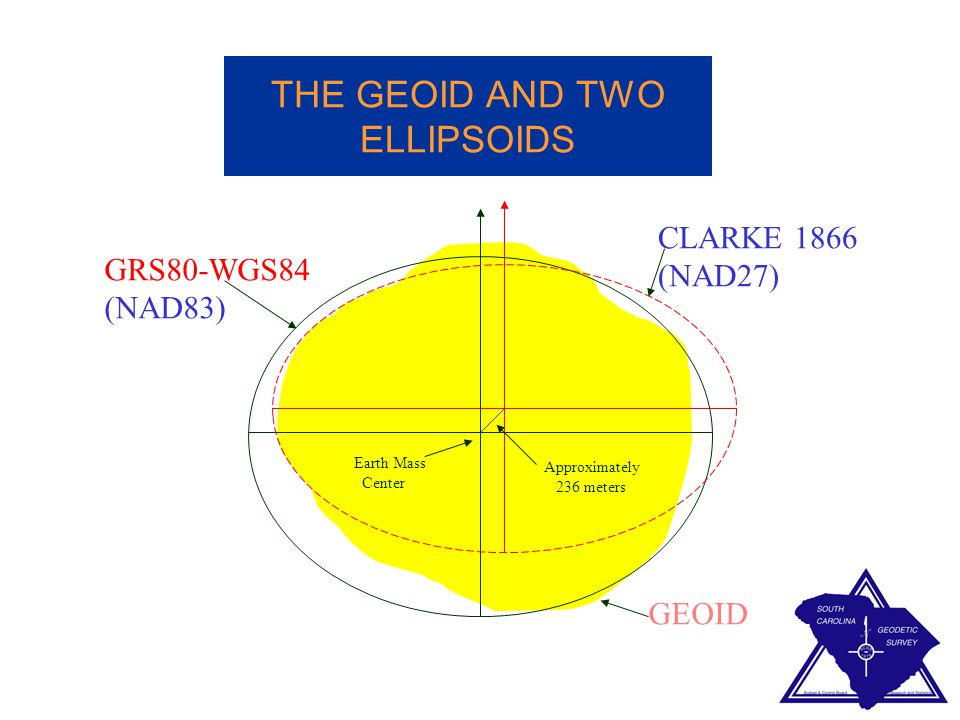
\includegraphics[width=13.33in]{C:/Users/a71386/Desktop/GeoHum/andres/geohumcourse/imgs/lokaalsed_globaalsed_daatumid} 

}

\caption{Erinevad daatumid: globaalne, geotsentriline WGS84 ja lokaalne NAD27 ([allikas](https://slideplayer.com/slide/3432120/))}\label{fig:daatumid}
\end{figure}

Daatumi ja sobiliku koordinaatsüsteemi abil saamegi määrata objektide asukohti Maa pinnal: teame, millise kujuga ja mõõtmetega kujutame Maad ette, ning teame ka, millistes ühikutes ja millisest nullpunktist lugedes me sellel kujul objektide asukohti määravaid koordinaate arvestame. \textbf{Geograafilised koordinaadid} on alati seotud mingi daatumiga ning aitavad meil määrata objekti asukoha, kasutades pikkus- ja laiuskraade. Pikkuskraade loetakse kahele poole Greenwichi observatooriumi meridiaani (idapikkus ja läänepikkus), laiuskraade kahele poole ekvaatorit (lõunalaius ja põhjalaius). Asukohta esitatakse kraadides (°), minutites (') ja sekundites (") või kraadides kümnendsüsteemis.

\textbf{Mõtteharjutus}:

\begin{quote}
Kui iga kraad on jagatud 60 minutiks ja iga minut 60 sekundiks, siis kuidas kujutada kümnendsüsteemis koordinaate 58°22'48``N, 26°43'20''E?
\end{quote}

Selleks aga, et nüüd geograafilises ruumis paiknevaid objekte kujutada tasapinnalisel mudelil ehk kaardil, peame valima kaardi \textbf{projektsiooni}, mis määrab viisi, kuidas sfääriline pink tasapinnal esitatakse ning kuidas ruumilised koordinaadid (GCS) konverteeritakse ümber \textbf{tasapinnalisteks koordinaatideks} (PCS ehk \emph{projected coordinate system}), mida väljendatakse \emph{x}-i ja \emph{y} abil. Sisuliselt määrab projektsioon ära ka selle, milliseid alasid maakeral me oleme nõus oma kaardil rohkem moonutama ja milliseid vähem ning mispidi me mingeid alasid kaardil venitame või kokku surume. Kui tahame kujutada ümmargust Maad kahemõõtmelisel tasapinnal, siis paratamatult peame mingit osa maakerast moonutama. Ühe või teise projektsiooni valimisel moonutame rohkem kas pindalasid, nurkasid, kujusid või joonpikkuseid.

\begin{figure}

{\centering 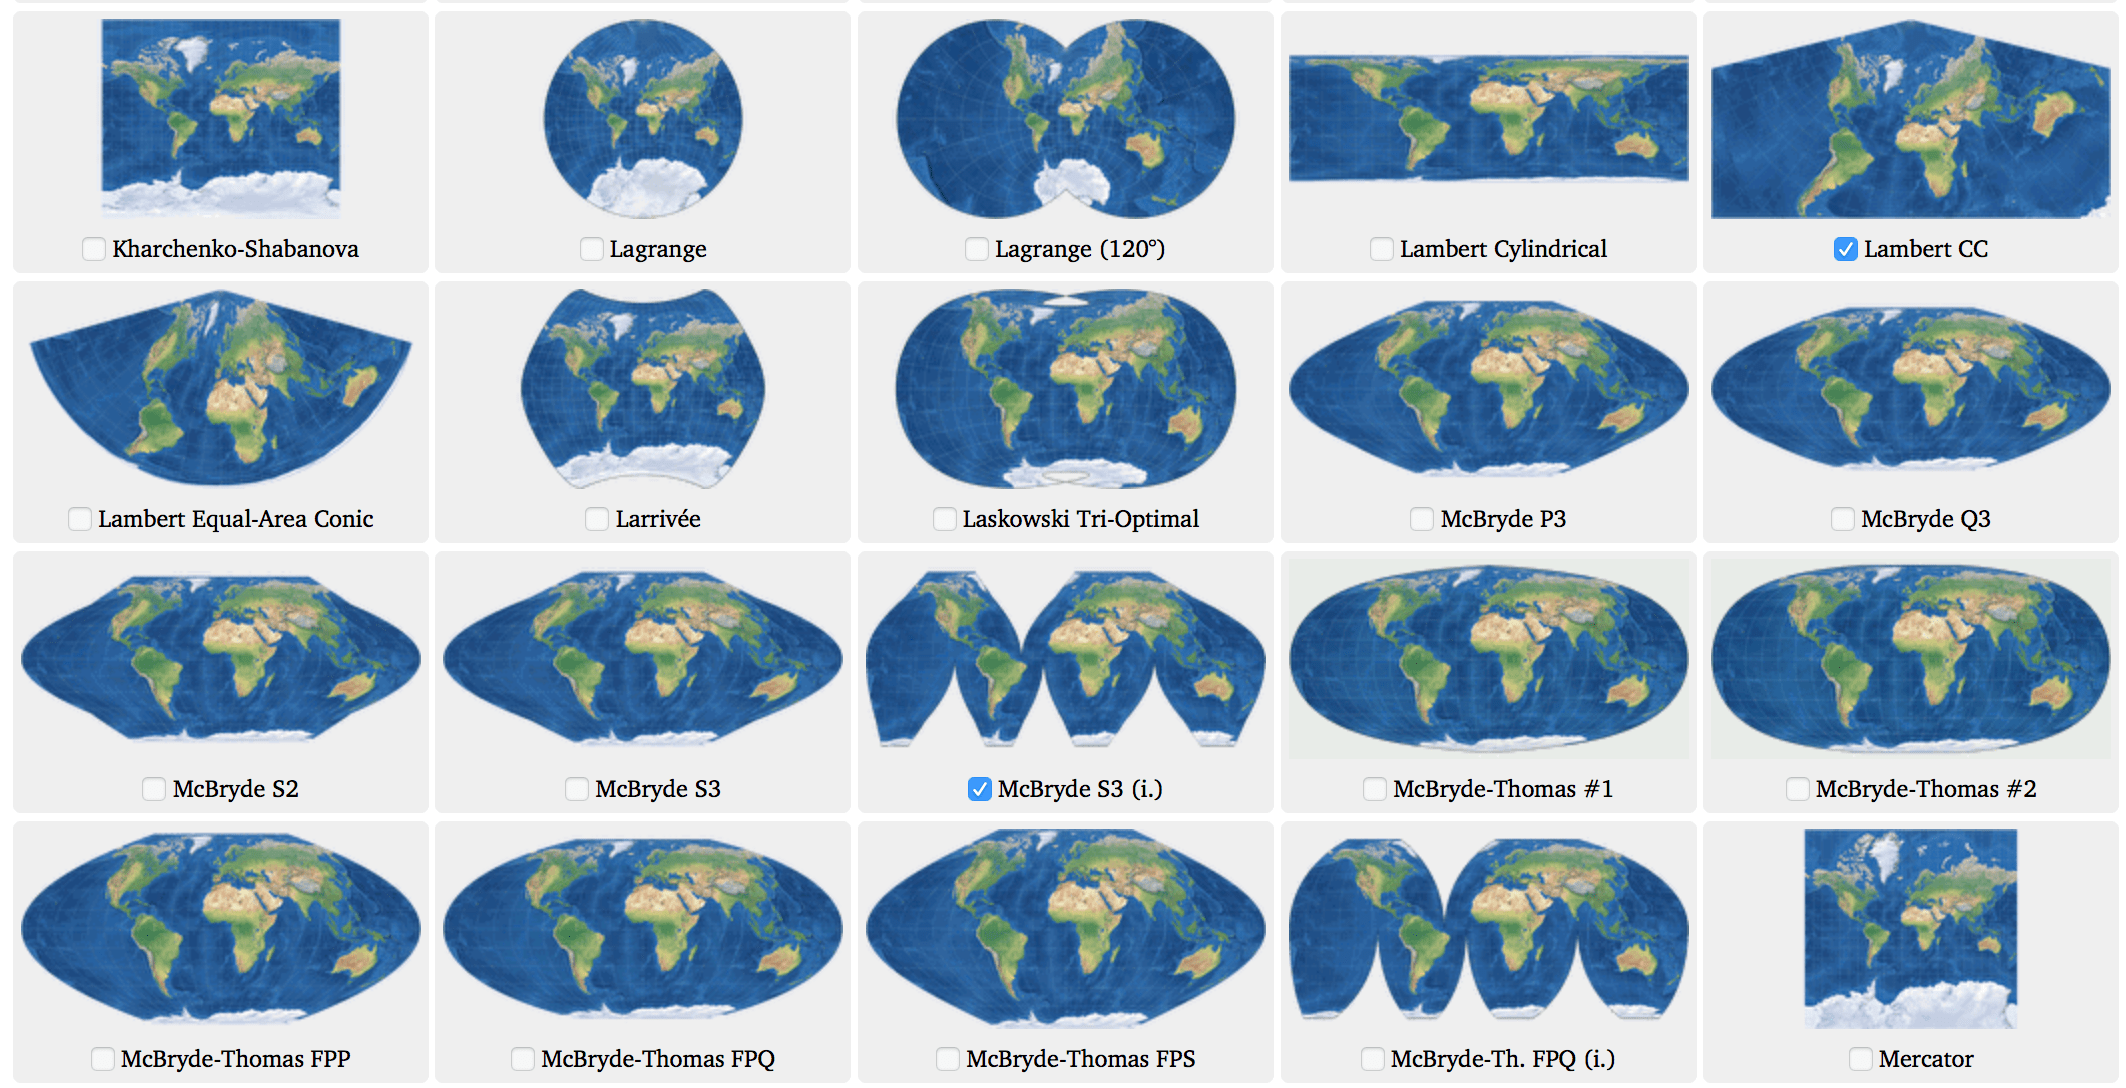
\includegraphics[width=1\linewidth]{C:/Users/a71386/Desktop/GeoHum/andres/geohumcourse/imgs/projections} 

}

\caption{[Erinevad projektsioonid](https://i.redd.it/8ssm7hfbeko21.png)}\label{fig:projections}
\end{figure}

Projektsioonid jagunevad üldisteks tüüpideks selle järgi, kas ruumilist maakera üritatakse projitseerida silindrile, koonusele või tasandile. Need üldised tüübid jaotatakse omakorda selle järgi, kuidas vastav siirdepind on maaellipsoidi suhtes orienteeritud (normaal-, põik- või kaldaspekt).

\begin{figure}

{\centering 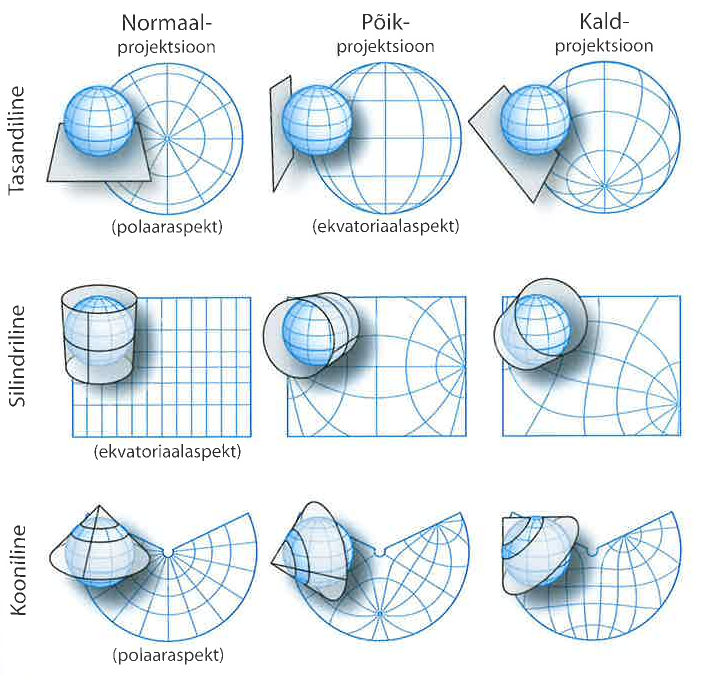
\includegraphics[width=1\linewidth,height=1\textheight]{C:/Users/a71386/Desktop/GeoHum/andres/geohumcourse/imgs/projektsiooniklassid} 

}

\caption{Projektsioonitüübid [@Aunap2019 : 169]}\label{fig:projektsioonipered}
\end{figure}

\begin{figure}

{\centering 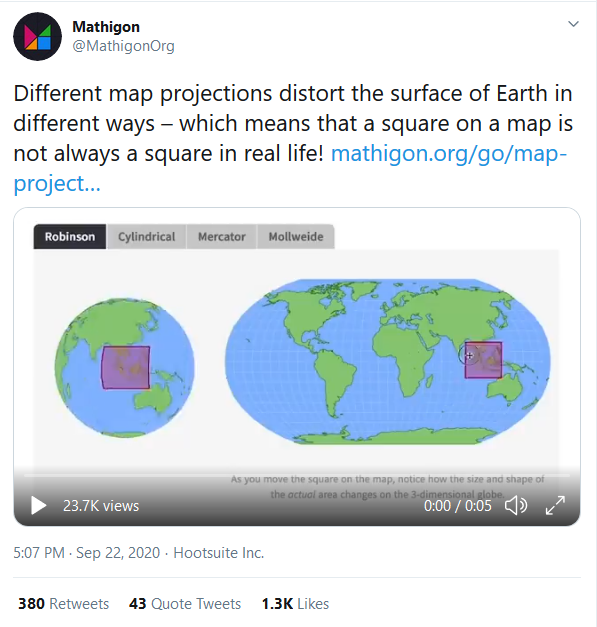
\includegraphics[width=0.7\linewidth,height=0.7\textheight]{C:/Users/a71386/Desktop/GeoHum/andres/geohumcourse/imgs/mathigontweet} 

}

\caption{Projektsioonide vahetamine [twitter.com/MathigonOrg](https://twitter.com/MathigonOrg/status/1308407528057901065)}\label{fig:mathigontweet}
\end{figure}

Lisaks n-ö kolmele geomeetrilisele põhiklassile on projektsioonide hulgas lisaks ka pseudoklasse, mis säilitavad ainult põhiklassi mõne tunnuse.

\begin{figure}

{\centering 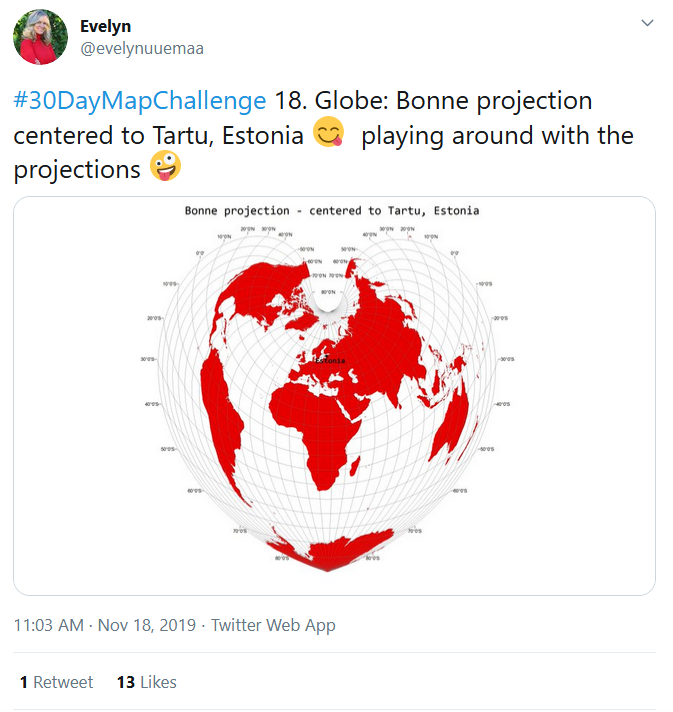
\includegraphics[width=0.7\linewidth,height=0.7\textheight]{C:/Users/a71386/Desktop/GeoHum/andres/geohumcourse/imgs/uuemaabonne} 

}

\caption{Bonne'i pseudokooniline projektsioon, mille keskmesse on pandud Tartu [twitter.com/evelynuuemaa](https://twitter.com/evelynuuemaa/status/1196353283696316416)}\label{fig:bonneprojection}
\end{figure}

Erinevatest projektsioonidest räägime kursuse jooksul lähemalt veel.

Lõpetuseks. GIS-tarkvarades kohtad mõistet \textbf{koordinaatide referentssüsteemi} (CRS - \emph{Coordinate reference system}), mis koosneb daatumist ehk Maa matemaatilisest mudelist ja projektsioonist, mis konverteerib geograafilised koordinaadid tasapinnalisteks koordinaatideks.

\hypertarget{veebipuxf5hised-kaardirakendused}{%
\section{Veebipõhised kaardirakendused}\label{veebipuxf5hised-kaardirakendused}}

Alati ei pea kaardi tegemiseks õppima põhjalikult tundma geoinfosüsteemide hingeelu ning kasutama mingit GIS-tarkvara. Veebis on valmis kaardirakendusi, mis võimaldavad teha ruumiandmete päringuid ja lihtsamaid analüüse (nt leia lühim/kiireim teekond punktist A punkti B), ilma et peaksid ise kaartide koostamise ja kujundamisega liiga palju vaeva nägema. Lisaks pakuvad mõned platvormid lisaks platvormi kaudu leitava info kasutamisele võimalust integreerida nendega ka enda andmeid ning kas või luua uusi ruumiandmeid. Lisaks sellele, et on võimalik enda andmeid n-ö olemasolevas süsteemis kuvada, pakuvad mõned platvormid võimalust ka ise aluskaardi tegemisel kaasa lüüa. Sellised on näiteks OpenStreetMap, WikiMapia ja Here WeGo, mis töötavad sarnaselt Vikipeediale: kasutajad saavad kaardi informatiivsust ja kvaliteeti ise parandada, lisades kaardile hooneid, teid jm objekte ning täiendades või parandades olemasolevate objektide infot.

Selles praktikumis vaatleme eelkõige veebirakendusi, mis võimaldavad teha lihtsamaid kaarte, mida võib siis esitada kas veebis või trükitult. Spetsiifiliselt veebilehtedel esitatavate kaartide tegemise võimalusi vaatame kursusel pisut hiljem.

Ilmselt kõige tuntum ja laialdasemalt kasutatav kaardirakendus on Google Maps, mille pakutavate teenuste hulka kuuluvad näiteks teekondade planeerimine (erinevate liiklusvahenditega), navigeerimissüsteem, liiklusinfo kuvamine, tänavate panoraamvaated, teatud kohtades ka veealused panoraamvaated ja siseruumide vaated, 45-kraadised aerofotod jm. Google Maps pakub ka võimalust võrdlemisi lihtsalt kuvada sobival aluskaardil enda andmeid. Seda võimalust vaatamegi esmalt lähemalt.

Vaatame sel korral koos esmalt just \textbf{\href{https://www.google.com/mymaps/}{Google Mapsi}} võimalusi ja seejärel võrdlete neid iseseisvalt teiste analoogsete rakendustega. Need on väga üldised kaardirakendused, mida kasutatakse kõiksugu erinevate teemakaartide loomiseks. Humanitaarteadlastele võiks eraldi aga pakkuda huvi ka pigem nende jaoks tehtud platvormid, nagu näiteks \href{http://hdlab.stanford.edu/palladio/}{Palladio}.

\hypertarget{google-my-maps}{%
\subsection{Google My Maps}\label{google-my-maps}}

Google My Maps on hea ja kiire variant vähenõudlikule kasutajale, kel on vaja koostada mingi teema kohta kaart, aga ei ole aega, et selleks spetsiaalselt mingit korralikku GIS-tarkvara kasutama õppida.

Kõige olulisemaks miinuseks on mõistagi see, et kasutajal on väga vähe kontrolli selle üle, missugune tema kaart välja näeb ja kuidas GM tema ruumiandmetega käitub. Samuti ei ole võimalik veebirakenduses oma ruumiandmeid analüüsida rohkem, kui arvutada võrdlemisi robustselt vahemaid ja teekondi.

Veebirakendus nõuab, et sul oleks Google'i konto.

Vaatame näitena üht väikest osa 19. sajandi teise poole Lõuna-Eesti vallakohtuprotokollidest, mille 2000. aastatel sisestas digitaalsel kujul Tõnis Türna (Rahvusarhiiv). 2016. aastal taastati algselt \emph{\url{http://www.history.ee/vallakohus}} lehel olnud protokollid veebiarhiivide põhjal ning katsetati nende peal eesti keele automaatset morfoloogilist analüsaatorit. Morfoloogilise analüsaatori ülesandeks on tunda ära sõnavorm ning pakkuda sellele sõnaraamatukuju, sõnaliigi, vormiinfot jm.

\begin{figure}

{\centering 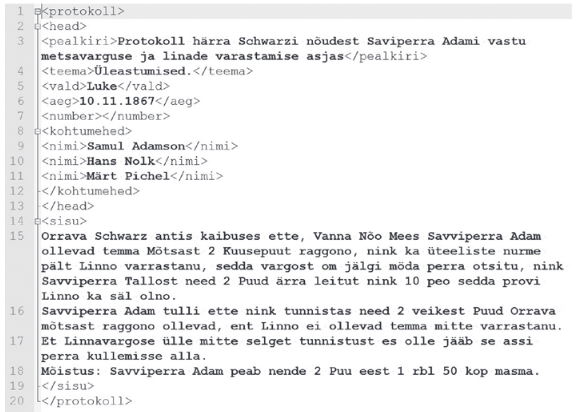
\includegraphics[width=1\linewidth]{C:/Users/a71386/Desktop/GeoHum/andres/geohumcourse/imgs/vallakohtuprotokoll} 

}

\caption{Vallakohtuprotokolli näide xml-kujul [@Pilvik2019]}\label{fig:protokoll}
\end{figure}

Automaatses analüüsis tundmatuteks jäänud sõnavormide osakaal on umbkaudseks indikaatoriks sellele, kui eripärane oli vastava protokolli keel tänapäeva keelest.

Saame lisada ka erinevaid andmekihte, näiteks Maa-ameti Geoportaalist alla laetavad maakonnapiirid (shp-formaadi oleme eelnevalt konverteerinud kml-failiks).

NB! Suuri faile ei saa lisada: 5Mb piir, mis sisuliselt jätab väga suure osa võimalikest ruumiandmetest välja.

\begin{figure}

{\centering \includegraphics[width=0.5\linewidth,height=1\textheight]{imgs/okt01_gif/gmaps1} \includegraphics[width=0.5\linewidth,height=1\textheight]{imgs/okt01_gif/gmaps2} 

}

\caption{Kaardi tegemine Google My Mapsis (1)}\label{fig:mymaps1}
\end{figure}

\begin{figure}

{\centering \includegraphics[width=0.5\linewidth,height=1\textheight]{imgs/okt01_gif/gmaps3} \includegraphics[width=0.5\linewidth,height=1\textheight]{imgs/okt01_gif/gmaps4} 

}

\caption{Kaardi tegemine Google My Mapsis (2)}\label{fig:mymaps2}
\end{figure}

\begin{figure}

{\centering \includegraphics[width=0.5\linewidth,height=1\textheight]{imgs/okt01_gif/gmaps5} \includegraphics[width=0.5\linewidth,height=1\textheight]{imgs/okt01_gif/gmaps6} 

}

\caption{Kaardi tegemine Google My Mapsis (3)}\label{fig:mymaps3}
\end{figure}

\begin{figure}

{\centering \includegraphics[width=0.5\linewidth,height=1\textheight]{imgs/okt01_gif/gmaps7} \includegraphics[width=0.5\linewidth,height=1\textheight]{imgs/okt01_gif/gmaps8} 

}

\caption{Kaardi tegemine Google My Mapsis (4)}\label{fig:mymaps4}
\end{figure}

\begin{figure}

{\centering \includegraphics[width=0.5\linewidth,height=1\textheight]{imgs/okt01_gif/gmaps9} \includegraphics[width=0.5\linewidth,height=1\textheight]{imgs/okt01_gif/gmaps10} 

}

\caption{Kaardi tegemine Google My Mapsis (5)}\label{fig:mymaps5}
\end{figure}

\begin{figure}

{\centering \includegraphics[width=0.5\linewidth,height=1\textheight]{imgs/okt01_gif/gmaps11} \includegraphics[width=0.5\linewidth,height=1\textheight]{imgs/okt01_gif/gmaps12} 

}

\caption{Kaardi tegemine Google My Mapsis (6)}\label{fig:mymaps6}
\end{figure}

\begin{figure}

{\centering \includegraphics[width=0.5\linewidth,height=1\textheight]{imgs/okt01_gif/gmaps13} \includegraphics[width=0.5\linewidth,height=1\textheight]{imgs/okt01_gif/gmaps14} 

}

\caption{Kaardi tegemine Google My Mapsis (7)}\label{fig:mymaps7}
\end{figure}

\hypertarget{uxfclesanne-1}{%
\subsection{Ülesanne}\label{uxfclesanne-1}}

Võrdle Google Mapsi teiste sarnaste platvormidega, nagu HERE WeGo (\href{https://mapcreator.here.com}{HERE Map Creator}), \href{https://www.pinmaps.net/mymaps/}{PinMaps}, \href{https://www.scribblemaps.com/}{Scribble Maps} või \href{https://www.zeemaps.com/}{ZeeMaps}. Võid julgelt kasutada ka Google'i abi (Vikipeedias näiteks on enamasti rakenduste funktsioonide loetelu ja ajoon üsna täpselt kirjeldatud). Abiks võib olla ka \href{https://en.wikipedia.org/wiki/Comparison_of_web_map_services}{see tabel}.

Lisa \href{https://padlet.com/maarjaliisapilvik/n1tpoyussyalbsc6}{Padletisse} testitud rakenduse kohta järgmist infot:

\begin{enumerate}
\def\labelenumi{\arabic{enumi}.}
\tightlist
\item
  Ligipääsetavus\\
\end{enumerate}

\begin{itemize}
\tightlist
\item
  kas rakenduse kasutamiseks peab registreerima?
\item
  kas mingite funktsioonide kasutamiseks peab maksma?\\
\item
  kas kasutamises on regionaalseid eripärasid? (mingid funktsioonid näiteks Eestis ei tööta või kaardi detailsusaste on väiksem)\\
\end{itemize}

\begin{enumerate}
\def\labelenumi{\arabic{enumi}.}
\setcounter{enumi}{1}
\tightlist
\item
  Kasutatavus
\end{enumerate}

\begin{itemize}
\tightlist
\item
  kui intuitiivne on kasutajaliides?
\item
  milliseid funktsioone rakendus pakub?\\
\end{itemize}

\begin{enumerate}
\def\labelenumi{\arabic{enumi}.}
\setcounter{enumi}{2}
\tightlist
\item
  Seosed teiste andmebaaside ja rakendustega
\end{enumerate}

\begin{itemize}
\tightlist
\item
  milliseid teisi platvorme ja andmebaase on rakendusse integreeritud?\\
\end{itemize}

\begin{enumerate}
\def\labelenumi{\arabic{enumi}.}
\setcounter{enumi}{3}
\tightlist
\item
  Muu
\end{enumerate}

\begin{itemize}
\tightlist
\item
  kui paljusid aluskaardi kihte on võimalik kuvada?\\
\item
  kas on võimalik lisada objekte?
\item
  kas on võimalik importida andmetabeleid?
\item
  millised piirangud andmetele on (nt formaat, failide maht jms)?
\item
  millised on ekspordivõimalused?
\item
  \ldots{}
\end{itemize}

Kui sul õnnestub teha mingite andmetega ka kaart, mida eksportida või jagada, siis võiksid panna ka selle oma sissekande juurde.

\begin{figure}

{\centering \includegraphics[width=1\linewidth,height=1\textheight]{C:/Users/a71386/Desktop/GeoHum/andres/geohumcourse/imgs/rakendustevordlus} 

}

\caption{Kaardirakenduste võrdlus}\label{fig:rakendused}
\end{figure}

\hypertarget{juxe4rgmisel-korral-2}{%
\section{Järgmisel korral}\label{juxe4rgmisel-korral-2}}

Esmaspäeval mõtiskleme veidi laiemalt kaartide mõiste üle ning uurime, kuidas saab kaardi abil lugusid jutustada (\emph{Story Maps}).

  \bibliography{kirjandus.bib}

\end{document}
